% Copyright (C) 2014-2024 by Thomas Auzinger <thomas@auzinger.name>

\documentclass[draft,final]{vutinfth} % Remove option 'final' to obtain debug information.

% Define convenience functions to use the author name and the thesis title in the PDF document properties.
\newcommand{\authorname}{Elias Huhsovitz} % The author name without titles.
\newcommand{\thesistitle}{Elastic Self-Adaptive Edge Pipelines} % The title of the thesis. The English version should be used, if it exists.

% Create the XMP metadata file for the creation of PDF/A compatible documents.
\begin{filecontents*}[overwrite]{\jobname.xmpdata}
\Author{\authorname}                                    % The author's name in the document properties.
\Title{\thesistitle}                                    % The document's title in the document properties.
\Language{de-AT}                                        % The document's language in the document properties. Select 'en-US', 'en-GB', or 'de-AT'.
\Keywords{a\sep list\sep of\sep keywords}               % The document's keywords in the document properties (separated by '\sep ').
\Publisher{TU Wien}                                     % The document's publisher in the document properties.
\Subject{Thesis}                                        % The document's subject in the document properties.
\end{filecontents*}

% Load packages to allow in- and output of non-ASCII characters.
\usepackage{lmodern}        % Use an extension of the original Computer Modern font to minimize the use of bitmapped letters.
\usepackage[T1]{fontenc}    % Determines font encoding of the output. Font packages have to be included before this line.
\usepackage[utf8]{inputenc} % Determines encoding of the input. All input files have to use UTF8 encoding.

% Extended LaTeX functionality is enables by including packages with \usepackage{...}.
\usepackage{amsmath}    % Extended typesetting of mathematical expression.
\usepackage{amssymb}    % Provides a multitude of mathematical symbols.
\usepackage{mathtools}  % Further extensions of mathematical typesetting.
\usepackage{microtype}  % Small-scale typographic enhancements.
\usepackage[inline]{enumitem} % User control over the layout of lists (itemize, enumerate, description).
\usepackage{multirow}   % Allows table elements to span several rows.
\usepackage{booktabs}   % Improves the typesetting of tables.
\usepackage{subcaption} % Allows the use of subfigures and enables their referencing.
\usepackage[ruled,linesnumbered,algochapter]{algorithm2e} % Enables the writing of pseudo code.
\usepackage[dvipsnames,table]{xcolor} % Allows the definition and use of colors. This package has to be included before tikz.
\usepackage{nag}        % Issues warnings when best practices in writing LaTeX documents are violated.
\usepackage{todonotes}  % Provides tooltip-like todo notes.
\usepackage{morewrites} % Increases the number of external files that can be used.
\usepackage[a-2b,mathxmp]{pdfx}      % Enables PDF/A compliance. Loads the package hyperref and has to be included second to last.
\usepackage[acronym,toc]{glossaries} % Enables the generation of glossaries and lists of acronyms. This package has to be included last.

% packages added by elias huhsovitz
\usepackage{float}

% used for tikz vector drawing
\usepackage{pgfplots}
\pgfplotsset{compat=1.18}

% Set PDF document properties
\hypersetup{
    pdfpagelayout   = TwoPageRight,           % How the document is shown in PDF viewers (optional).
    linkbordercolor = {Melon},                % The color of the borders of boxes around hyperlinks (optional).
}

\setpnumwidth{2.5em}        % Avoid overfull hboxes in the table of contents (see memoir manual).
\setsecnumdepth{subsection} % Enumerate subsections.

\nonzeroparskip             % Create space between paragraphs (optional).
\setlength{\parindent}{0pt} % Remove paragraph indentation (optional).

\makeindex      % Use an optional index.
\makeglossaries % Use an optional glossary.
%\glstocfalse   % Remove the glossaries from the table of contents.

% Set persons with 4 arguments:
%  {title before name}{name}{title after name}{gender}
%  where both titles are optional (i.e. can be given as empty brackets {}).
\setauthor{}{\authorname}{}{male}
% \setadvisor{Univ.Prof. Dr.}{Schahram Dustdar}{}{male}
\setadvisor{Proj.Ass. Dr.}{Boris Sedlak}{}{male}

% For bachelor and master theses:
% \setfirstassistant{Proj.Ass. Dr.}{Boris Sedlak}{}{male}
%\setsecondassistant{Pretitle}{Forename Surname}{Posttitle}{male}
%\setthirdassistant{Pretitle}{Forename Surname}{Posttitle}{male}

% For dissertations:
\setfirstreviewer{Pretitle}{Forename Surname}{Posttitle}{male}
\setsecondreviewer{Pretitle}{Forename Surname}{Posttitle}{male}

% For dissertations at the PhD School and optionally for dissertations:
\setsecondadvisor{Pretitle}{Forename Surname}{Posttitle}{male} % Comment to remove.

% Required data.
\setregnumber{12121272}
\setdate{23}{07}{2025} % Set date with 3 arguments: {day}{month}{year}.
\settitle{Elastic Stream Processing Pipelines for Heterogeneous Edge Devices}{}
%\settitle{\thesistitle}{Elastic Stream Processing Pipelines for Heterogeneous Edge Devices} % Sets English and German version of the title (both can be English or German). If your title contains commas, enclose it with additional curvy brackets (i.e., {{your title}}) or define it as a macro as done with \thesistitle.
%\setsubtitle{} % Sets English and German version of the subtitle (both can be English or German).

% Select the thesis type: bachelor / master / doctor.
% Bachelor:
\setthesis{bachelor}
%
% Master:
%\setthesis{master}
%\setmasterdegree{dipl.} % dipl. / rer.nat. / rer.soc.oec. / master
%
% Doctor:
%\setthesis{doctor}
%\setdoctordegree{rer.soc.oec.}% rer.nat. / techn. / rer.soc.oec.

% For bachelor and master:
\setcurriculum{Software \& Information Engineering}{Software \& Information Engineering} % Sets the English and German name of the curriculum.

% Optional reviewer data:
\setfirstreviewerdata{Affiliation, Country}
\setsecondreviewerdata{Affiliation, Country}


\begin{document}

\frontmatter % Switches to roman numbering.
% The structure of the thesis has to conform to the guidelines at
%  https://informatics.tuwien.ac.at/study-services

%\addtitlepage{naustrian} % German title page.
\addtitlepage{english} % English title page.
\addstatementpage

%\begin{danksagung*}
%\todo{Ihr Text hier.}
%\end{danksagung*}

\begin{acknowledgements*}
I would like to thank my supervisor, Dr. Boris Sedlak, for his guidance and helpful feedback during the development of this thesis.

I also thank Felix Berger and Tobias Seczer for their valuable non-technical feedback, particularly regarding figure layout and document presentation.
\end{acknowledgements*}

%\begin{kurzfassung}
%\todo{Ihr Text hier.}
%\end{kurzfassung}


\begin{abstract}
Edge computing is increasingly essential for handling real-time data streams generated by IoT devices, mobile applications, and sensor networks. However, edge environments are characterized by constrained computational resources, hardware heterogeneity, and unpredictable workloads. These conditions make it difficult to maintain Service Level Objectives (SLOs) such as latency, memory usage, and throughput. Traditional elasticity mechanisms, such as horizontal autoscaling, are ill-suited to such scenarios due to the inability to provision additional resources at will. This creates a need for a principled, interpretable approach to dynamic control that can uphold system constraints while maximizing Quality of Experience (QoE).

This thesis introduces a distributed, parallel stream processing pipeline for real-time video inference on edge systems. A central Active Inference (AIF) agent governs the elasticity of stream quality parameters, such as frame rate, resolution, and inference quality, by minimizing expected free energy to balance SLO satisfaction and stream quality. The agent encodes SLOs as prior preferences and continuously updates its generative model through online learning. The prototype is evaluated in three scenarios: stable operation, dynamic demand shifts, and fluctuating compute budgets. Compared to a heuristic baseline, the AIF agent achieves higher global SLO compliance and maintains more stable configurations in moderately dynamic conditions. Under high volatility, limitations begin to show and highlight the potential of future extensions with decentralized inference. Overall, the work demonstrates that Active Inference provides a robust and generalizable control paradigm for elastic, self-adaptive edge pipelines under uncertainty.
\end{abstract}



% Select the language of the thesis, e.g., english or naustrian.
\selectlanguage{english}

% Add a table of contents (toc).
\tableofcontents % Starred version, i.e., \tableofcontents*, removes the self-entry.

% Switch to arabic numbering and start the enumeration of chapters in the table of content.
\mainmatter

% link to chapters
\chapter{Introduction}

\section{Motivation}
The rapid growth of Internet of Things (IoT) devices, mobile computing applications, and real-time sensor networks has led to an exponential increase in data streams generated at the edge of the network. As a consequence, edge computing has emerged as a distributed paradigm, wherein processing and decision-making are performed as close as possible to data sources \cite{deng_edge_2020}. The core promise of edge computing lies in its capacity to
reduce latency, enhance privacy, save bandwidth, and improve responsiveness by processing data closer to the sources of generation \cite{deng_edge_2020}. 

However, edge computing introduces its own set of challenges. Unlike the virtually
elastic resources of centralized data centers, edge devices are highly heterogeneous \cite{furst_elastic_2018},
resource-constrained in terms of compute, memory, and energy availability and operate in unpredictable environments \cite{sedlak_active_2024, danilenka_adaptive_2025}. This complexity is exacerbated by Quality of Service (QoS) and Quality of Experience (QoE) standards that modern edge computing scenarios must sustain. The ability to provide high-quality service under such conditions is critically dependent on the capacity to monitor, predict, and enforce Service Level Objectives (SLOs)—quantitative targets, such as latency, throughput, and resource utilization \cite{sedlak_diffusing_2024, nastic_sloc_2020}. 

Ensuring SLO compliance in these environments is an unsolved problem. The necessity of elasticity—that is, dynamically scaling application parameters or resources in response to workload fluctuations and SLO states—demands new control paradigms that are both data-driven and interpretable \cite{lapkovskis_benchmarking_2025, dias_de_assuncao_distributed_2018}.

Traditional solutions, such as threshold-based scaling or Reinforcement Learning (RL), often fail to provide robust guarantees or require costly retraining under shifting environmental conditions \cite{xu_coscal_2022}. Moreover, they often do not possess adequate predictive capabilities, making real-time adaptation difficult under rapidly changing workloads and operational conditions \cite{oquinn_environment-aware_2025}.

In response to these limitations, advanced approaches that incorporate predictive and adaptive
capabilities are necessary. Active Inference (AIF), a concept derived from neuroscience, as introduced by Karl J. Friston in \cite{friston_free-energy_2010}, has recently emerged as a methodology to address such challenges. AIF provides a unified mathematical framework enabling agents to
continually anticipate and adapt to uncertainty through perception-action cycle \cite{friston_active_2016, lanillos_active_2021}. This thesis addresses the challenge of integrating AIF principles in a distributed system environment to adapt resource allocation and maintain QoS and QoE under strict constraints.

\section{Challenges and Problem Definition}
Designing adaptive edge systems for real-time data streams presents several key
challenges. First, edge environments are highly heterogeneous \cite{furst_elastic_2018}, with varying capabilities and
rapidly shifting workloads \cite{danilenka_adaptive_2025}. Especially as Artificial Intelligence (AI) expands into the edge, it creates a heightened demand for high-performance, low-latency inference across devices \cite{oquinn_environment-aware_2025}. Second, unlike in centralized settings, edge systems must make do with varying resource pools \cite{sedlak_equilibrium_2024}.

Traditional distributed computing frameworks, such as MapReduce \cite{dean_mapreduce_2008},
Apache Storm\cite{noauthor_apache_nodate} and Apache Flink \cite{noauthor_apache_nodate-1, carbone_apache_2015}, have significantly advanced the parallelization and
distribution of data-intensive computations. Nevertheless, these frameworks were initially
developed for environments with relatively abundant resources and predictable workloads,
making their direct application to highly dynamic edge scenarios challenging. Conventional elasticity management practices, which often involve heuristic-based rules or reactive scaling methods, are insufficient to address the adaptation requirements of edge computing environments. Sedlak et al. mention in \cite{sedlak_diffusing_2024} the fact that there is still a significant lack of integrated frameworks that combine predictive modeling, real-time inference, dynamic elasticity, and strict SLO enforcement. As a result, there is a strong need for comprehensive methods that use advanced prediction to proactively manage resources and maintain performance in the constrained conditions of edge computing.

This relates to the third major challenge \textit{continuous adaptation}\cite{danilenka_adaptive_2025}. A popular alternative to Heuristic agents are Machine Learning (ML) based approaches to adapt the system. However, as Sedlak et al. observe in \cite{sedlak_active_2024}, these approaches fail to capture gradual changes in the environment, as long as the ML models are not retrained, leading to an inaccurate view of the system. This creates the need for an agent that continuously adapts to its environment \cite{sedlak_equilibrium_2024}.

\section{Research Question and Objectives}
\label{sec:research-question}
Given the outlined challenges and research gaps, the primary objective of this thesis is to
investigate how Active Inference can be effectively applied to resource-constrained edge
computing environments for the predictive control of elasticity and the enforcement of
Service Level Objectives. Specifically, the thesis seeks to address the central research question:

\begin{quote}
\textit{
How can data streams be processed efficiently in resource-limited edge computing environments using Active Inference to dynamically control elasticity and uphold explicit Service Level Objectives (SLOs) to maintain Quality of Experience (QoE)?
}
\end{quote}

To answer this question, this thesis pursues the following objectives:
\begin{itemize}
    \item Design and implement a distributed, parallel pipeline for stream processing on edge
devices
    \item Employ SLOs as first-class constraints to enforce resource, and latency
requirements across components of the pipeline.
    \item  Introduce an elasticity mechanism that can dynamically adapt core stream
processing parameters to match workload and resource conditions.
    \item Leverage active inference (AIF), to govern elasticity and ensure continuous fulfillment of SLOs.
    \item Evaluate the effectiveness of this approach in upholding quality standards
and resource constraints under realistic edge workloads by using a video stream processing prototype based on YOLO object detection.
\end{itemize}

\section{Proposed Approach}
This thesis proposes a novel distributed parallel pipeline architecture for edge data stream processing, which is tightly coupled with a real-time elasticity mechanism governed by an active inference agent. In this architecture, data streams are partitioned and processed in parallel across multiple worker nodes. Each worker executes inference or transformation tasks, while a collector node aggregates the results. Crucially, a central agent continuously monitors SLOs and system state, and adjusts stream parameters to maximize Quality of Experience (QoE). To balance the resource- and QoE requirements, the system implements Service Level Objectives (SLOs), a fundamental concept used to meet the performance and quality targets of the system \cite{sedlak_towards_2025, nastic_sloc_2020}.

The distinguishing contribution of this work is the application of active inference as a generic,
explainable control paradigm for adaptive elasticity. By framing SLO satisfaction and quality maximization as explicit preferences within a generative model, the agent is able to select actions that balance exploitation (maximizing stream quality) and exploration (reducing model uncertainty), in accordance with current observations and beliefs \cite{casamayor_pujol_deepslos_2024, sedlak_adaptive_2024, danilenka_adaptive_2025, lanillos_active_2021}. This approach is generalizable to arbitrary data streams (including audio, video, sensor, or network data), and can support a range of SLO types and system constraints.


\chapter{Background}
The three core mechanisms used for dynamically adjusting stream processing in this thesis are Service Level Objectives (SLOs), Elasticity and Active Inference (AIF). This chapter introduces foundational concepts, essential for understanding how Active Inference
can be effectively leveraged to uphold Service Level Objectives (SLOs) in resource-constrained
edge computing environments. The first section establishes the critical role of SLOs in edge computing scenarios. The subsequent section defines the role of Elasticity in Edge Computing Systems. The penultimate section explores all of the key concepts regarding Active Inference and the Free Energy Principle. The final section discusses the principles for using AIF in distributed systems.

\section{Edge Computing and Service Level Objectives}
Edge computing refers to a distributed computing paradigm in which data processing occurs in
close proximity to the data source. This architectural shift reduces the latency and bandwidth
limitations inherent in centralized cloud computing \cite{deng_edge_2020}, while enabling real-time
analytics for latency-sensitive tasks such as autonomous driving, smart surveillance, and
industrial automation \cite{zhang_octopus_2023}.

Edge computing environments are characterized by pronounced heterogeneity \cite{furst_elastic_2018} , i.e, resource-asymmetry, vendor specifications, and usage patterns \cite{danilenka_adaptive_2025}. Devices may range from embedded computing boards to more capable edge servers, each
with distinct resource constraints in terms of CPU, memory, energy, bandwidth and especially GPU, which has become a significant factor due to increasing inference demand. When tasked with continuous stream
processing (e.g., real-time video analysis), such systems must dynamically manage
computational demands without the luxury of cloud-level resource elasticity.

To formalize quality expectations in such constrained environments, Service Level Objectives
(SLOs) are used \cite{casamayor_pujol_deepslos_2024}. SLOs define quantifiable thresholds on performance metrics, such as
response time, memory usage, or energy consumption targets \cite{danilenka_adaptive_2025}. SLOs serve as internal optimization goals \cite{danilenka_adaptive_2025} to guide system behavior under varying load conditions \cite{nastic_sloc_2020}.
For example, in a video inference pipeline, one
might define an SLO that memory usage must remain below 80\% of available capacity.

Crucially, SLOs can serve a dual role: they can be targets for optimization and/or constraints that the
system must not violate \cite{casamayor_pujol_deepslos_2024, sedlak_diffusing_2024}. In edge scenarios, where stream quality competes directly with resource availability, such as video streaming tasks \cite{sedlak_adaptive_2024}, SLO-aware control is essential \cite{sedlak_slo-aware_2025}.

\section{Elasticity in Edge Computing Systems}
Elasticity refers to a system’s ability to automatically adapt to changing workloads and resource availability. Since edge devices typically operate under fixed compute budgets, scaling hardware resources is not an option. Thus, elasticity must be achieved through intelligent control of software parameters \cite{sedlak_towards_2025}.

Sedlak et al. define elasticity in \cite{sedlak_towards_2025} along multiple axes:
\begin{itemize}
  \item \textbf{Quality Elasticity} — adjusts application-level parameters such as resolution, FPS,
or inference model complexity
  \item \textbf{Resource Elasticity} — modulates CPU, memory, or I/O usage
  \item \textbf{Cost Elasticity} — optimizes for energy efficiency or execution time.
\end{itemize}

Each elasticity action impacts both the system's SLO fulfillment and its Quality of Experience
(QoE). For instance, reducing the inference model complexity alleviates computational load but may lead to less accurate results. The key challenge lies in selecting the most appropriate elasticity action under uncertainty, while maintaining SLO compliance and maximizing QoE.

Traditional control mechanisms, such as threshold-based rules, static policies or Mache Learning approaches are not optimal to address this trade-off in dynamic environments \cite{sedlak_active_2024}. A model-based approach, capable of learning and adapting to evolving contexts, is therefore required \cite{sedlak_equilibrium_2024, danilenka_adaptive_2025}.

\section{Active Inference and the Free Energy Principle}
\subsection{The Free Energy Principle}
The Free Energy Principle (FEP), as defined in \cite{friston_free-energy_2010}, provides a unified
theory of perception, action, and learning. It posits that any self-organizing system that
maintains equilibrium with its environment over time must minimize the long-term divergence between its
internal beliefs and external sensory states \cite{friston_active_2017}. This divergence, known as
surprise, refers to the difference between what an agent predicts based on its internal model and what it observes in the environment \cite{sedlak_adaptive_2024}.

\subsubsection{Generative Process and Model}
Agents cannot minimize surprise directly, since the actual way that the world produces sensory data
is unknown. This process that describes the true causes for how the world generates observable
outcomes is known as the \textit{generative process} \cite{friston_free-energy_2010, smith_step-by-step_2022}. As an agent is unable to observe the ``real world``, it instead creates an internal representation of the \textit{generative process}, known as the \textit{generative model}. The \textit{generative model} serves as an approximation and is used by the agent to predict and adjust its environment according to its preferences.

\begin{figure}[htbp]
    \centering
    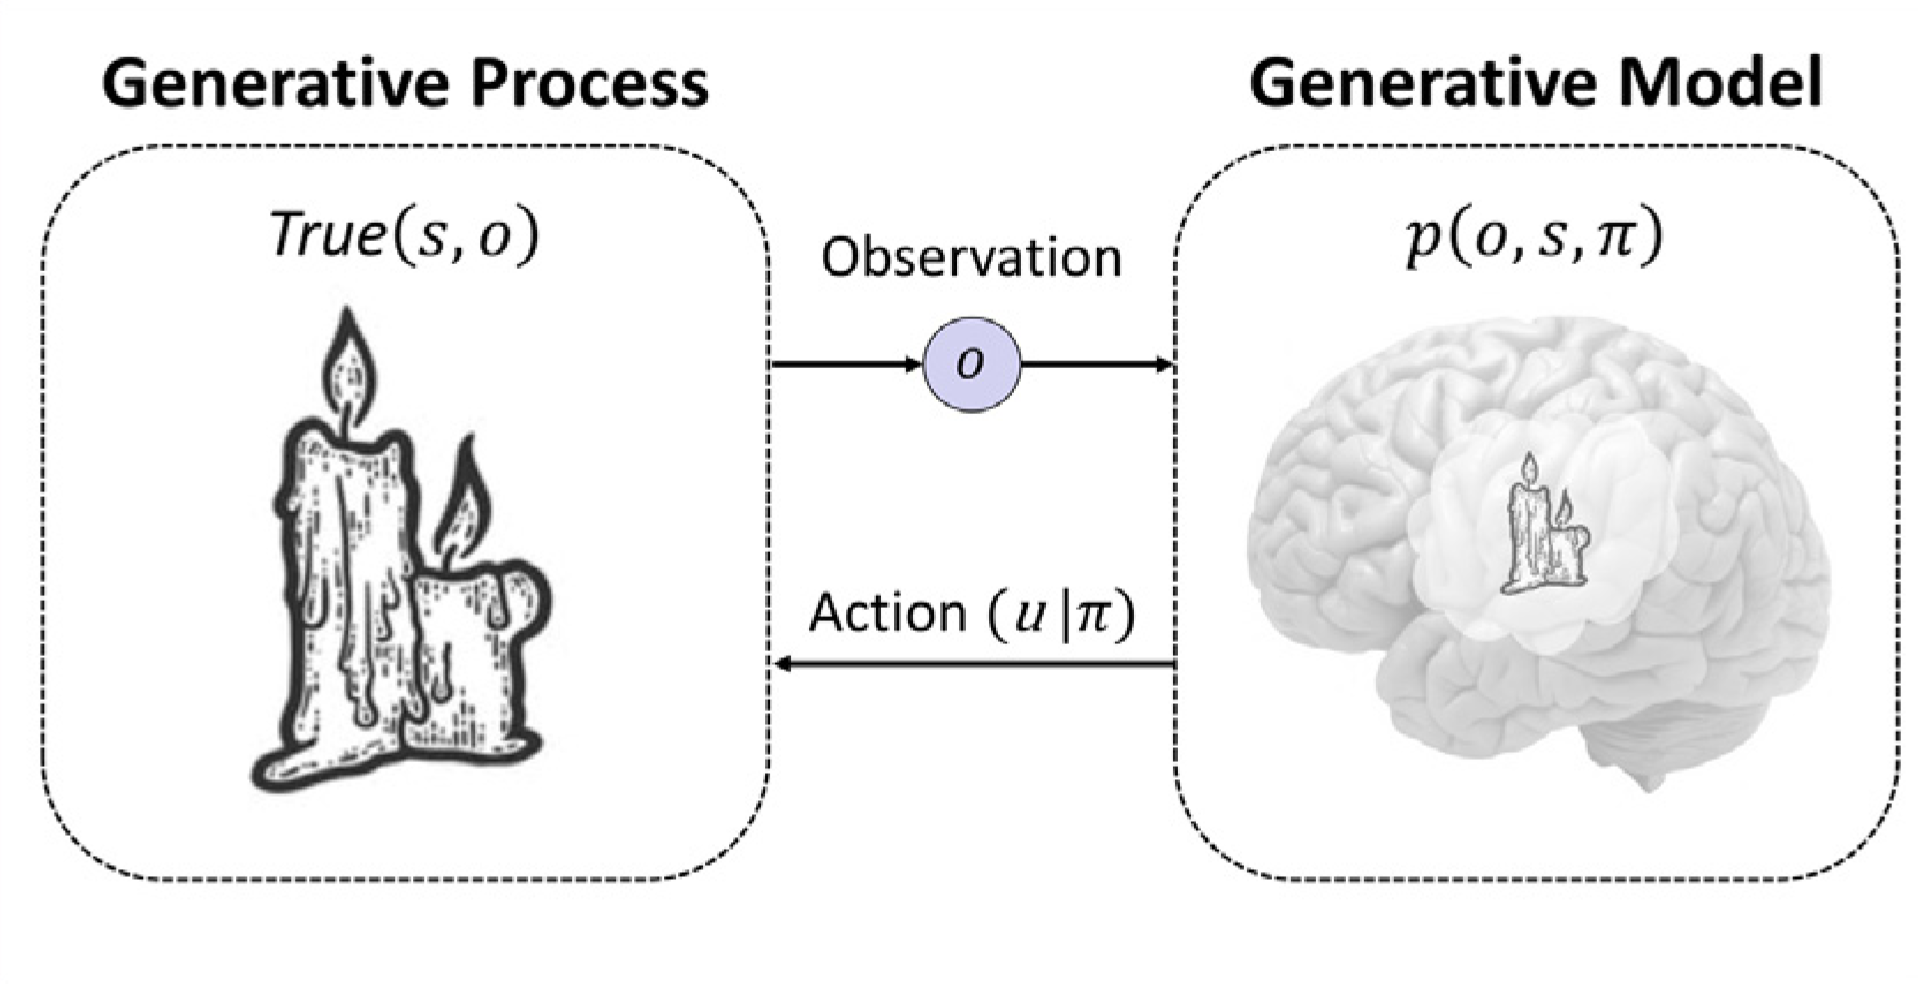
\includegraphics[width=0.8\textwidth]{img/generative-model-generative-process.png}
    \caption{Distinction and implicit coupling of generative process and the generative model. (taken from \cite{smith_step-by-step_2022})}
    \label{fig:generative-process-generative-model}
\end{figure}

When the \textit{generative process} and the \textit{generative model} differ, the agent will be ``surprised``, causing it to adjust its model closer towards the process \cite{bruineberg_free-energy_2018}. The closer the generative model is to the underlying generative process, the higher the precision of the agent's predictions is \cite{sedlak_active_2024}.

\subsubsection{Free Energy minimization}
To align the \textit{generative models} with the \textit{generative process}, the agent aims to reduce surprise to the maximum extent. A system cannot directly evaluate surprise, because this would require knowing all hidden states of the world \cite{friston_free-energy_2009}, i.e. the \textit{generative process}. Instead, an agent aims to 
minimize an upper bound \cite{smith_step-by-step_2022} known as (variational) Free Energy (FE). It captures the difference between the agent's internal representation of the world and its observations, making it a computationally feasible substitution for surprise. Therefore, by minimizing FE, agents implicitly minimize surprise \cite{friston_free-energy_2010}


FE can be expressed as the Kullback-Leibler (KL) divergence between approximate posterior probability (Q) of hidden states (x) and their exact posterior probability (P) \cite{sedlak_active_2024, sedlak_adaptive_2024,sajid_active_2021}. 
\[FE = TODO Formula and variables for Free Energy\]

 minimizing free energy minimizes KL divergence and brings the agent’s beliefs closer to the true posterior distribution \(TODO: Distribution Variables here\).

 \subsubsection{Expected Free Energy}
To act in the world, agents must not only evaluate current states but also anticipate the outcomes of future actions. This is done via Expected Free Energy (EFE). EFE extends the concept of variational Free Energy into the future, by evaluating possible future action sequences using a policy \(\pi\). \cite{friston_active_2016}. The agent uses the EFE to decide on actions. EFE is made up of two key components \cite{friston_active_2022} % Active Inference: The Free Energy Principle in Mind, Brain, and Behavior%
\begin{enumerate}
  \item \textbf{Epistemic Value (Information Gain)} — Drives exploration by favoring actions that are expected to yield informative outcomes, improving the agent’s generative model.
  \item \textbf{Pragmatic Value} — Drives the agent to select actions that are likely to fulfill its explicit goals or preferences, i.e., it promotes exploitation.
\end{enumerate}

Together, these terms enable the agent to balance the classic exploration-exploitation tradeoff \cite{sedlak_adaptive_2024}. This dual drive allows AIF
agents to maintain SLOs while learning optimal control strategies for software parameters. \cite{lapkovskis_benchmarking_2025}.

\subsection{Active Inference}
Active inference (AIF) operationalizes the Free Energy Principle in artificial agents, extending it to encompass both state estimation and action selection \cite{sedlak_equilibrium_2024, lanillos_active_2021}. To implement the concepts of the Free Energy Principle, an agent maintains a \textit{generative model}, which includes the following categorical distributions \cite{heins_pymdp_2022}:

\begin{itemize}
  \item \textbf{Observation model \(P(o \mid s)\):} Defines how the hidden states produce observations and allows the agent to infer what it expects to see, given its beliefs about the world. Specifically, the likelihood model specifies the probability of an observation \(o\) given a hidden state \(s\). 
  \item \textbf{Transition model \(P(s_{t+1} \mid s_t,a_t)\):} Defines how hidden states evolve over time, depending on the actions taken by the agent. Specifically, the likelihood model explains: If the agent is in state \(s_t\) and takes action \(a_t\), what is the probability that it will end up in state \(s_{t+1}\). 
  \item \textbf{Prior preferences over observations \(P(o)\):} The agent's preferences, encoded as preferred observations (e.g., SLO fulfillment). Action selection is biased by this preference distribution, leading agents to choose actions that bring them to states that (they expect) will lead to preferred observations. It returns the numerical preference for a given observation \(o\).
  \item \textbf{Prior beliefs about hidden states \(P(s_0)\):} The initial beliefs about the environment. This is the starting point that the agent uses for inference at the first time step. It returns the probability of being in state \(s_0\).
  \item \textbf{Prior beliefs about policies: \(P(\pi)\):} Expectations about the outcomes of possible sequences. It biases the agent toward certain policies before observing anything or computing EFE. Useful for modeling habits, biases, or repetition.
\end{itemize}

\subsubsection{The Active Inference loop}
To decrease EFE and consequently align the \textit{generative model} with the \textit{generative process}, the agent repeatedly engages in an action-perception loop \cite{sedlak_equilibrium_2024}. Figure \ref{fig:acive-inference-loop} provides a high-level overview. During each cycle, the agent performs three main steps \cite{heins_pymdp_2022}:
\begin{enumerate}
    \item \textbf{Perception:} Sampling an observation from the environment.
    \item \textbf{Belief updating:} Updating the agent’s beliefs about states and policies using the
observation.
    \item \textbf{Action:} Choosing and executing actions that minimize EFE, based on the agent’s posterior over policies.
\end{enumerate}

This loop is executed at regular intervals during an agent's lifetime. As Bruineberg et al. summerize in \cite{bruineberg_free-energy_2018}: ``This gives rise to a continuous feedback loop, in which what the agent does changes the environment, which changes what the agent perceives, which changes the expectations of the agent, which in turn changes what the agent does (to change the environment).``

\begin{figure}[htbp]
    \centering
    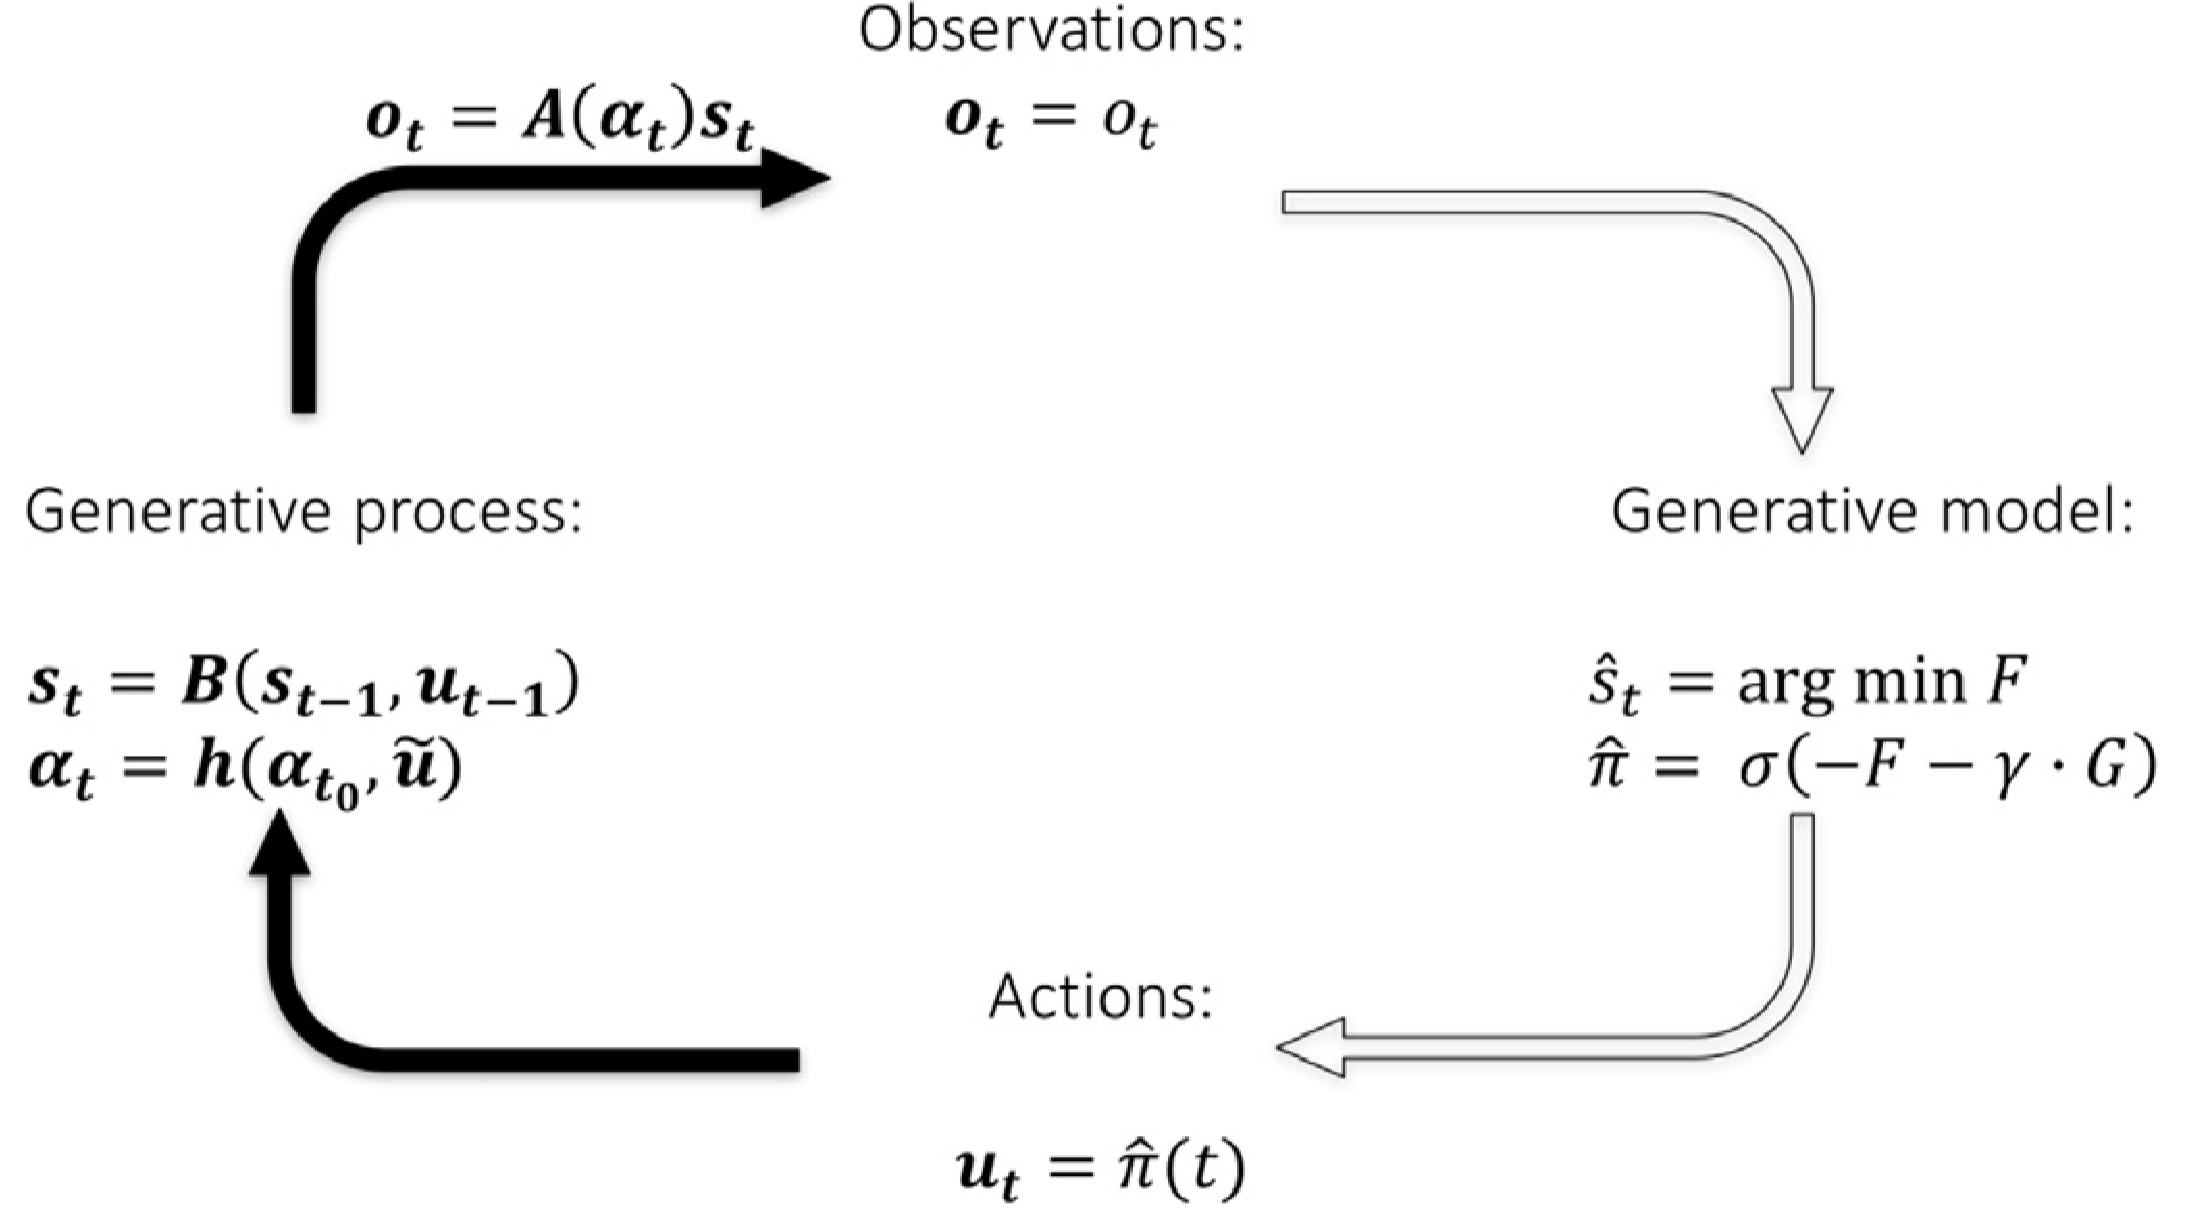
\includegraphics[width=0.8\textwidth]{img/active-inference-loop.png}
    \caption{The Active Inference loop. (taken from \cite{bruineberg_free-energy_2018})}
    \label{fig:acive-inference-loop}
\end{figure}

\section{Active Inference in Distributed Systems}
The application of active inference (AIF) to distributed systems, such as edge pipelines or multi-agent infrastructures, enables robust and interpretable control in dynamic and resource-constrained environments. Distributed systems often consist of asynchronous components with overlapping responsibilities, limited observability, and evolving workloads—conditions that challenge traditional rule-based or purely data-driven control methods. AIF addresses these challenges by equipping agents with generative models that capture the causal relationships between system parameters (e.g., processing configurations) and observed outcomes (e.g., SLO satisfaction). By interacting with the environment and updating beliefs, agents learn how their actions affect system behavior. This iterative action-perception cycle allows agents to adapt to their environment during their lifetime. As Sedlak et al. note in \cite{sedlak_active_2024}, “The agent used causal knowledge to gradually develop an understanding of how its actions are related to requirements fulfillment, and which configurations to favor”.

In distributed edge pipelines, AIF agents can operate locally, managing a single node or service, or hierarchically, coordinating across components to optimize system-level objectives. In both cases, adaptation is driven by minimizing EFE. This balances two goals: maximizing the probability of fulfilling preferences (i.e., SLOs and QoE goals) and reducing uncertainty about the system \cite{friston_free-energy_2010, lanillos_active_2021}. 

This thesis implements a single-agent variant of this framework: an AIF controller monitors the global state of a distributed stream processing pipeline and dynamically adjusts elasticity parameters that impact the quality of the system's output. The agent intervenes when SLOs (e.g., memory constraints) approach critical levels and selects adaptations that restore compliance while improving its generative model \cite{sedlak_equilibrium_2024}.

Although focused on a centralized AIF controller, the underlying framework is inherently extensible to multi-agent settings, where distributed agents can share beliefs or synchronize generative models. Prior work has demonstrated how such agents can collaboratively manage resources and task assignments in real-time systems while maintaining local autonomy and decentralized control \cite{sedlak_slo-aware_2025}. Such concepts will be discussed in chapter\ref{chap:related-work}

\chapter{Related Work}
\label{chap:related-work}
This chapter provides an overview of key literature relevant to Elasticity and AIF within distributed and edge computing contexts. While AIF has found wide application in robotics and cognitive systems \cite{lanillos_active_2021}, its adoption in edge computing remains sparse. Notable progress in applying elasticity through AIF in resource-constrained environments emerged primarily through the work of Sedlak et al. \cite{sedlak_adaptive_2024, sedlak_equilibrium_2024, sedlak_active_2024, sedlak_slo-aware_2025, lapkovskis_benchmarking_2025, sedlak_towards_2025}, Danilenka et al. \cite{danilenka_adaptive_2025}, and to a certain extent, Levchuk et al. \cite{levchuk_active_2019} in multi-agent Internet
of Things (IoT) systems. Given the early stage of AIF in edge computing, this chapter focuses on a selected set of foundational and state-of-the-art contributions to contextualize the motivation and relevance of our approach.

\section{Runtime adaptation of stream processing systems}
Runtime adaptation allows stream processing services to continuously adapt to changing workloads and environments. Cardellini et al.~\cite{cardellini_runtime_2022} review a wide range of techniques that systems use to adapt at runtime. These include resource scaling, relocating operators across devices, skipping or dropping data under overload (load shedding), and fine-tuning system parameters like buffer size or batch interval. Adaptation can be managed centrally by a global controller or locally by decentralized agents, and can be triggered either in reaction to performance violations or in anticipation of them.

Early implementations such as DivProg by Fürst et al.~\cite{furst_elastic_2018} demonstrate heuristic-based adaptation using function annotations and a code selection engine. Their elastic services dynamically switch between classifier types and image resolutions to meet latency constraints across heterogeneous edge devices.

Cao et al.~\cite{cao_neural_2023} present RL-Adapt, a framework that trains reinforcement learning models to generate adaptation policies targeting application-specific QoE metrics. Their system operates in real time on constrained IoT hardware, adjusting parameters like frame rate and compression quality.

\section{Elasticity for stream processing under SLO constraints}
In \cite{sedlak_towards_2025}, Sedlak et al. extend this approach, presenting a control architecture where services can adapt along multiple dimensions of elasticity, i.e., resource- and quality-elasticity. The system dynaimcally adjusts configuration parameters such as the number of allocated CPU cores (\textit{cpu}) and the resolution of the video stream (\textit{pixels}). These two controllable parameters, along with the frame rate (\textit{fps}) of the video stream, are used as SLO targets for the stream processing services. Actions are selected based on a combination of Deep Reinforcement Learning and a reward function, based on SLO fulfillment. Rather than relying solely on vertical autoscaling, their framework uses elasticity as a first-class mechanism to operate under fixed-resource budgets typical of edge nodes. This work also introduces the idea of causally linking low-level service parameters with high-level application goals.

\section{Active Inference as a unified approach for edge adaptation}
In \cite{sedlak_active_2024}, Sedlak et al. present a design study for applying Active Inference (AIF) to edge computing systems with a focus on maintaining Service Level Objectives (SLOs) in resource-constrained environments. They propose a self-evidencing agent that operates in an action-perception cycle, using a generative model to predict system behavior, compare outcomes with expectations, and update beliefs to minimize free energy. The agent’s preferences are encoded directly as SLOs, guiding both its predictions and actions. The framework explicitly links system metrics—such as batch delay and utilization—to causal structures, enabling interpretability and continuous adaptation without requiring pretraining. This approach distinguishes itself from traditional ML systems by integrating causal reasoning, homeostasis, and epistemic exploration into a unified control loop. This design study provides the blueprint for implementing AIF-based control in edge computing scenarios.

Complementing this theoretical design, \cite{sedlak_adaptive_2024} presents an implemented and evaluated AIF agent for adaptive stream processing on edge devices. Their system dynamically adjusts stream quality parameters—specifically frame rate (fps), resolution (pixel), and processing mode—based on the agent’s generative model and its beliefs about system behavior. SLOs such as latency, energy consumption, and detection accuracy are encoded as preferred observations (priors), guiding the agent’s policy selection through the minimization of EFE. The action-perception cycle allows the agent to iteratively update its beliefs and reconfigure services in response to observed deviations, thereby ensuring consistent SLO fulfillment across heterogeneous devices and workloads. This work directly informs the methodology of this thesis, which adopts a comparable architectural approach and operationalizes SLOs in a similar way to enable self-adaptive control.



\chapter{Methodology}
\label{chap:methodology}

This chapter presents a general framework for upholding Service Level Objectives (SLOs) in distributed stream processing pipelines deployed in edge computing environments. The methodology addresses the central research question \ref{sec:research-question} of this thesis. To provide an answer, this thesis proposes a unified architecture that combines parallel stream processing with Active Inference (AIF)–based adaptive control. This architecture is designed to elastically adjust system behavior to uphold SLOs in the face of limited computational resources and dynamic workloads. It is designed to be generic, extensible, and applicable across a wide variety of real-time data stream applications at the edge.

\section{System Architecture}
This section outlines the core architectural components of the proposed framework. It details how data is ingested, processed, and aggregated within a distributed streaming pipeline. The design emphasizes modularity, scalability, and responsiveness under constrained resources.

\subsection{Pipeline Design and Parallel Processing}
At the core of our framework lies a modular streaming pipeline composed of three functionally distinct entities: a\textbf{ Producer}, a set of parallel \textbf{Workers}, and a \textbf{
Collector}. The Producer generates a continuous stream of data segments, so-called \textit{tasks}, and enqueues them for processing. A \textit{task} generated by the producer is a simple data structure containing an id, an instruction, and a chunk of data from the underlying stream. The Workers operate in parallel and independently process each task according to the current parameter configurations. Once processed, results are transmitted asynchronously to the Collector, which reassembles and delivers the final output. 

This modular separation enables horizontal scalability and encapsulation of concerns: the Producer governs stream rate and complexity, the Workers handle computation, and the Collector ensures ordering and completion. This design is inspired by the dataflow paradigm typical in modern stream processing systems, such as Apache Storm \cite{carbone_apache_2015, noauthor_apache_nodate}. 

Figure \ref{fig:methodology-parallel-distributed-pipeline} provides a high-level overview of the design.

\begin{figure}[htbp]
    \centering
    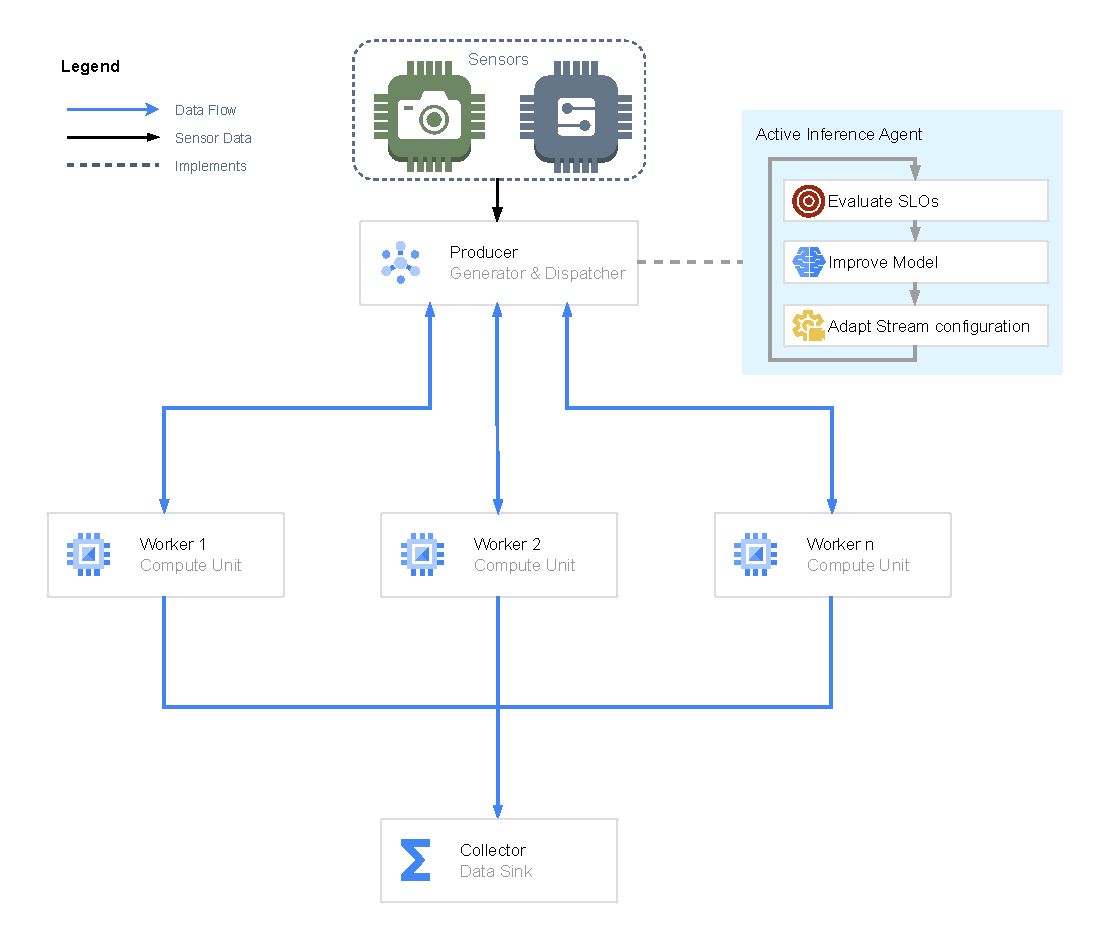
\includegraphics[width=\textwidth]{img/methodology/methodology_parallel_pipeline_overview.drawio.pdf}
    \caption{Overview of system architecture describing (1) request-reply communication between producer and worker, (2) collection of results by the collector, (3) action-perception cycle of the AIF agent.}
    \label{fig:methodology-parallel-distributed-pipeline}
\end{figure}


\subsection{Task Distribution and Load Balancing}
Tasks are distributed in a decentralized fashion: each worker node actively requests tasks when ready to compute, forming a pull-based load balancing model. This mechanism enables the system to scale to a large number of workers without requiring global synchronization. This load-balancing pattern emerges naturally as faster or less burdened nodes consume more tasks \cite{estrada_comparing_2015}.

While such an architecture increases communication overhead, as the worker node has to go out of its way to request data, it also enables efficient utilization of heterogeneous compute resources by aligning task assignment with runtime capacity.

\subsection{Asynchronous Communication Model}
All communication between components is asynchronous. Producers dispatch tasks without blocking \cite{lauener_how_2018}; workers process and return results independently; and collectors operate on incoming data streams without waiting on global completion barriers.

This asynchronous design supports robustness under dynamic conditions, such as fluctuating task loads or varying network bandwidth \cite{nguyen_octopinf_2025}. This non-blocking operation is critical for real-time scenarios in which latency constraints must be maintained regardless of individual node performance fluctuations.


\subsection{Multi-Dimensional Elasticity}
Due to the resource-constrained nature of edge computing environments, vertical or horizontal scaling techniques cannot be used to uphold SLOs. To fulfill SLOs, the system must dynamically adapt the computational demand to fit the system's resource budget, meaning specific parameters need to be modifiable during runtime.

This requires that each stream processing task supports multiple execution configurations, each with associated performance characteristics and requirements. A configuration defines a set of \textit{stream quality parameters}, such as inference quality, task frequency and task size. All of these parameters directly impact QoE and computational demands. The system supports multi-dimensional elasticity, meaning that these parameters can be individually tuned during runtime.

The Producer operates as the central controller of stream parameterization. The changing of stream parameter can be separated into two types:

\begin{itemize}
    \item \textbf{Task generation:} Stream parameters that directly affect the generation of tasks are changed directly at the producer level. The configuration then affects all newly generated tasks.
    \item \textbf{Task processing:} Stream parameters that affect large changes on the worker, such as switching inference quality, require coordination between producer and worker. When the producer dictates a change, it enqueues a control task, detailing the nature of the change, in the \textit{backlog}\label{def:backlog} of each worker. The next time a worker requests a task from the producer, it receives the control tasks and makes the described changes, before continuing with normal stream processing. This ensures synchronized configuration among workers.
\end{itemize}

\section{Active Inference-Based Elasticity Control}

The system exposes control of the \textit{stream quality parameters} to the AIF agent (As depicted in figure~\ref{fig:methodology-parallel-distributed-pipeline} at the producer). 

\subsection{Generative Model Construction}
Central to a capable AIF agent is the construction of the \textit{generative model}. It represents the causal relationships between system configuration parameters and observable SLO metrics. It captures both direct (i.e., quality parameters) and indirect dependencies (i.e., SLO) affecting agent behavior. This model includes:
\begin{itemize}
  \item \textbf{Observation model \(P(o \mid s)\):} Obeservations of Stream Paramters and SLO values.
  \item \textbf{Transition model \(P(s_{t+1} \mid s_t,a_t)\):} Actions taken by Agent to change stream quality paramters.
  \item \textbf{Prior preferences over observations \(P(o)\):} Agent prefers high stream quality paramters, while strongly averting unfilled SLOs.
  \item \textbf{Prior beliefs about hidden states \(P(s_0)\):} The initial state of SLOs and stream quality parameters, before any data has been processed.
  \item \textbf{Prior beliefs about policies: \(P(\pi)\):} 
\end{itemize}

\subsubsection{Prioritization Strategy}
Crucially, the SLOs and \textit{stream quality parameters} are encoded as prior preferences with different absolute values. The preference to fulfill an SLO must be equally as strong, or slighty stronger than the preference to increase the quality of the stream (i.e., increase computational demand). This results in a lexicographic prioritization, where the primary objective is to maintain SLOs and the secondary objective of maximizing \textit{stream quality parameters}. This prioritization reflects the insight that QoE directly correlates with increased computational cost. Therefore, aggressive maximization of \textit{stream quality parameters} without constraint awareness would lead to SLO violations and system degradation.

The relationship between configuration and SLO fulfillment is non-linear. Therefore, the system must learn which configurations fulfill SLOs under which conditions, and which trade-offs are most efficient \cite{sedlak_towards_2025}.

\subsection{Continous Observation and Configuration Adjustment}
The AIF loop~\ref{sec:active-inference-loop} is executed periodically during the producer's runtime to evaluate and adapt the system's configuration. Finding an appropriate interval between evaluations is critical, as it determines how frequently the agent can revise and apply its control policy. Short intervals (e.g., 50\,ms) allow rapid responsiveness but risk instability. Actions may be issued faster than their causal effects can propagate through the system, leading to overcompensation or oscillatory behavior. This is especially problematic in stream processing pipelines where SLO-relevant variables such as memory usage evolve with delay. Conversely, overly long intervals (e.g., 5\,s) hinder the system’s ability to respond to rapid environmental changes, potentially causing SLO violations due to latency in corrective actions. The implementation in chapter~\ref{chap:implementation} executes an action-perception cycle every 500\,ms.

\subsubsection{Active Inference Loop}
Each iteration of the loop involves a three-step procedure: observation, state and policy inference, and action sampling.

This sub-section describes the cycle based on the \texttt{pymdp} \cite{heins_pymdp_2022}, a python library implementing AIF for Markov Decision Processes. It serves as a great abstraction for this explanation and is later utilized in the implementation~\ref{sec:evaluation-implementation-active-infernce-agemt}. This choice does not constrain the generality of the proposed methodology. The loop structure, model components, and control logic are independent of any specific framework and can be implemented using alternative tools or custom inference routines. However, \texttt{pymdp} offers a modular and transparent interface for constructing Active Inference agents in discrete state spaces, well-suited to the modeling assumptions underlying this work. Its use in this thesis serves both as a practical vehicle for experimentation and as a clear reference implementation of the conceptual model described. 

\begin{enumerate}
    \item \textbf{Observation Sampling (Peception):} The agent receives updated observations from the environment via the Producer. These include current values for the stream quality parameters and the normalized SLO values. The observations are then encoded in \(o_t\).

    \item \textbf{Belief Updating over States and Policies:} The agent updates its beliefs about hidden states $s_t$ using the latest observation \(o_t\), applying variational Bayesian inference to approximate the posterior \(Q(s_t)\). This is handled via:
    \begin{quote}
        \texttt{agent.infer\_states(\(o_t\))}
    \end{quote}
    Subsequently, the agent infers a posterior distribution over policies $\pi$, each representing a sequence of actions (e.g., changing inference quality) over a receding horizon. Policies are evaluated by their expected free energy $\mathbb{G}(\pi)$, which integrates both \emph{epistemic value} (information gain) and \emph{instrumental value} (goal fulfillment). Policies minimizing expected free energy are preferred. This step is implemented via:
    \begin{quote}
        \texttt{agent.infer\_policies()}
    \end{quote}
     Policies that minimize anticipated SLO violations while improving QoE are preferred.

     In addition, the agent updates its generative model by refining its beliefs about the observation and transition probabilities through
    \begin{quote}
        \texttt{agent.update\_A(\(o_t\))} \\
        \texttt{agent.update\_B(\(Q(s_t)\))}
    \end{quote}
    
    \item \textbf{Action Selection:} The agent samples the most promising action from the posterior over policies and executes the first action in the sequence. This corresponds to reconfiguring the stream pipeline by adjusting stream parameters. Execution is performed via:
    \begin{quote}
        \texttt{action = agent.sample\_action()}
    \end{quote}
    The action is then translated into a concrete command that is either applied to the task generation template or inserted as a control task into the worker backlog (see Section~\ref{def:backlog}).
\end{enumerate}

\subsubsection{Homeostasis}
The agent's long-term objective is the persistent minimization of \textit{surprise} \cite{sedlak_adaptive_2024}, achieving homeostasis. This is done by finding a configuration that maximizes QoE, while upholding all SLOs.
\chapter{Implementation}
\label{chap:implementation}
This chapter presents the implementation of the proposed methodology outlined
in chapter~\ref{chap:methodology}. It demonstrates the feasibility of using Active Inference (AIF) to dynamically manage elasticity in distributed edge pipelines while upholding Service Level Objectives (SLOs). A Python-based prototype simulates a real-time video processing system and compares the AIF agent to baseline control strategies under constrained edge conditions.

The prototype of the distributed pipeline and the experimental results are available in a publicly accessible repository \footnote{The prototype of the stream processing framework is available at \href{https://github.com/JohnnyElaine/bsc_aif_parallel_pipeline}{GitHub}, accessed on July 22nd 2025.}.


The prototype implements a parallel and distributed processing pipeline inspired by Apache Flink~\cite{carbone_apache_2015}. It processes video streams using YOLOv11 inference and dynamically controls elasticity via an AIF agent deployed at the producer.

\section{System Architecture}
The architecture consists of three roles:
\begin{itemize}
    \item \textbf{Producer:} Splits the frames of the video stream into tasks, and dispatches them to workers. It also acts as the central controller of elasticity and exposes control of the \textit{stream quality parameters} to its AIF agent.
    \item \textbf{Workers:} Execute YOLOv11 inference on received tasks and sends the result to the Collector.
    \item \textbf{Collector:} Aggregates processed results into an ordered output stream.
\end{itemize}

Communication is fully asynchronous and implemented using ZeroMQ sockets~\cite{noauthor_zeromqpyzmq_nodate}. Task dispatch from the Producer to Workers uses the REQ-ROUTER pattern, forming a pull-based work distribution model, also known as a Load-Balancing Pattern. Processed results are forwarded from Workers to the Collector using the PUSH-PULL pattern. This design ensures that work is allocated based on each worker’s readiness, optimizing system responsiveness and throughput.

ZeroMQ sockets are multiplexed using event loops, allowing simultaneous listening and sending. Task payloads (NumPy arrays) are transmitted as raw binary data without any copying, by leveraging the buffer interface they implement. Task metadata is serialized using msgpack \cite{noauthor_msgpackmsgpack-python_nodate} for compact binary transport.


TODO: Figure of the overall system architecture

\section{Producer Architecture}
The producer fulfills three roles: task generation, elasticity control, and agent orchestration.

\subsection{Task Queue and Generation}
A continuous stream of video frames is segmented into tasks and temporarily stored in a FIFO queue. Each \texttt{Task} includes:
\begin{itemize}
    \item \texttt{type:} Task purpose (e.g., INFERENCE, COLLECT).
    \item \texttt{id:} Unique identifier.
    \item \texttt{stream\_key:} Identifier for multi-stream support.
    \item \texttt{data:} A video frame, as a NumPy \texttt{ndarray}.
\end{itemize}
The number of tasks generated per second is dependent on the current configuration of the \textit{fps} parameter. Tasks are served upon worker request and consumed from the queue.

\subsection{Service Level Objectives}
Table~\ref{tab:slo-table} shows 4 types of SLOs intending to guarantee the QoE. These SLOs serve as constraints that guide the elastic adaptation process of the producer, helping to maintain a balance between processing quality and system stability.

\begin{table}[h]
    \centering
    \begin{tabular}{@{}lll@{}}
        \toprule
        \textbf{Var.} & \textbf{Rel.} & \textbf{Description} \\
        \midrule
        \textit{memory usage} 
            & \( \leq \theta_\text{mem} \) 
            & container memory usage \\
            
        \textit{task queue size} 
            & \( \leq \textit{fps} \cdot \varepsilon_\text{queue} \) 
            & task queue size \\
            
        \textit{avg process time} 
            & \( \leq \frac{1}{\textit{fps}} \cdot \varepsilon_\text{global}\) 
            & average global processing time \\
            
        \textit{highest avg process time} 
            & \( \leq \frac{1}{\textit{fps}} \cdot \varepsilon_\text{worker}\) 
            & worker with the highest average processing time \\
        \bottomrule
    \end{tabular}
    \caption{Service Level Objectives (SLOs) at the producer}
    \label{tab:slo-table}
\end{table}


The \textbf{Memory Usage SLO} ensures that the container does not exceed a specified memory capacity \(\theta_\text{mem}\). This protects the system from memory saturation, which would cause severe performance degradation as tasks might be offloaded to slower storage or dropped entirely.

\paragraph{Task Queue Size SLO}
Ensures that the number of unprocessed tasks remains within a reasonable limit, based on the current \textit{fps} parameter and a tolerance \(\varepsilon_\text{queue}\). A growing queue indicates that the processing capacity of the workers is insufficient for the current workload. This SLO acts as a safeguard for maintaining real-time responsiveness. The tolerance threshold must be set low enough to avoid the accumulation of multiple seconds worth of unprocessed frames in the task queue. At the same time, it must be sufficiently permissive to prevent immediate reactions to minor fluctuations, such as transient network delays. Based on empirical evaluation, a recommended tolerance range for the queue size SLO is \( 2 \geq \varepsilon_\text{queue} \geq 4\).

\paragraph{Average Global Task Processing Time SLO} Ensures that, on average, all workers combined can keep pace with the input stream. It is computed by tracking the processing time of the most recent \(n\) completed tasks using a moving average window. These statistics are reported by each worker during regular task requests. The goal is to ensure that the cumulative system throughput is sufficient to maintain real-time responsiveness. \(\varepsilon_\text{global}\) denotes a tolerance factor. A recommended value is \(\varepsilon_\text{global} = 1\), meaning the average time to process a single task must not exceed the current task generation time interval. Violations of this SLO indicate that the aggregate compute capacity of the system is insufficient to sustain the current input rate. This SLO serves as a holistic throughput constraint, ensuring that the pipeline as a whole can process frames as quickly as they arrive.

Violations of this SLO indicate that the aggregate compute capacity of the system is insufficient to sustain the current input rate. This SLO serves as a holistic throughput constraint, ensuring that the pipeline as a whole can process frames as quickly as they arrive.

\paragraph{Highest Per-Worker Average Task Processing Time SLO} Enforces an upper bound on the slowest worker’s performance. It ensures that no individual worker lags so far behind that its results become irrelevant to the output stream. This is particularly important in distributed pipelines, where late-arriving results may be discarded if the collector has already progressed past the corresponding task ID.

Here, \(\varepsilon_\text{worker} \geq 1\) provides additional tolerance compared to the global SLO. A typical setting is \(\varepsilon_\text{worker} = 4\), allowing slower nodes to process a task in up to 4 times the time budget permitted by the frame rate. By ensuring that even the slowest node performs within tolerable bounds, the system can maintain temporal coherence and avoid dropping results from late workers.

TODO: explain 3 SLO states (OK, WARNING, CRITICAL)

\subsection{Elasticity and Stream Parameter Control}
The \textit{Producer} serves as the central control entity for elasticity. It continuously monitors and adjusts three key \textit{quality parameters} of the video stream: (1) frames per second (\textit{fps}), (2) \textit{resolution}, and (3) \textit{inference quality}. While the producer directly sets fps and resolution by modulating task generation frequency and resizing video frames, inference quality refers to the YOLOv11 model variant employed by the worker nodes, e.g., \texttt{LOW} $\rightarrow$ \texttt{YOLOv11n}, \texttt{MEDIUM} $\rightarrow$ \texttt{YOLOv11s}, \texttt{HIGH} $\rightarrow$ \texttt{YOLOv11m}.

Although inference is executed on the workers, the producer dictates the inference quality of the entire system. To enforce a configuration change, it maintains a dedicated \textit{backlog} for each worker node. When the producer initiates a change (e.g., \texttt{MEDIUM} $\rightarrow$ \texttt{LOW}), it inserts the entry \texttt{CHANGE\_INFERENCE\_QUALITY=LOW} into the backlog of every registered worker. Upon the next task request, the worker's backlog is evaluated. If a configuration change is pending, the producer replies with a message of type \texttt{CHANGE} detailing all configuration changes the worker needs to make. This includes \texttt{CHANGE\_INFERENCE\_QUALITY=LOW}, instructing the worker to adapt its local inference model accordingly. Once the change is applied, the worker resumes normal task processing.

This design ensures that all nodes operate under a globally consistent inference configuration while minimizing coordination overhead.

\subsection{Active Inference Agent}
\label{sec:evaluation-implementation-active-infernce-agemt}
The control of the \textit{quality parameters} is delegated to the AIF agent running on the producer. Its objective is to uphold all defined Service Level Objectives (SLOs) while maximizing the Quality of Experience (QoE) through adaptive control of frame rate (FPS), resolution, and inference quality. The agent is implemented using pymdp \cite{heins_pymdp_2022} and operates continuously, executing one action-perception cycle every 500\,ms. Each cycle results in no action or a change in \textit{stream quality parameters}. 

\paragraph{Generative Model Construction.}
The agent operates a \textit{generative model} comprising the following components:
\begin{itemize}
  \item \textbf{Observation model \(P(o \mid s)\):} SLO values and quality parameters
  \item \textbf{Transition model \(P(s_{t+1} \mid s_t,a_t)\):} Latent configuration state
  \item \textbf{Prior preferences over observations \(P(o)\):} Strong preference for high quality parameters and equally strong aversion for SLO violations
  \item \textbf{Prior beliefs about hidden states \(P(s_0)\):} Inital quality parameter configuration.
\end{itemize}

\paragraph{Discrete State and Action Space Construction.}
Each configuration of the system is represented as a tuple of discrete quality parameter values:
\begin{itemize}
  \item \textbf{Frame Rate (FPS)} $\in \{$480p, 720p, 1080p$\}$
  \item \textbf{Resolution} $\in \{$10, 15, 20, 25, 30$\}$
  \item \textbf{Inference Quality} $\in \{$LOW, MEDIUM, HIGH$\}$
\end{itemize}

\paragraph{Actions}
The AIF agent operates using a \textit{relative control} strategy. Rather than selecting absolute parameter values, each action proposes an incremental change along one of the quality parameter dimensions. Specifically, the agent can:

\begin{itemize}
  \item \textbf{Frame Rate (FPS):} increase, decrease, or retain the current FPS setting.
  \item \textbf{Resolution:} increase, decrease, or retain the current resolution setting.
  \item \textbf{Inference Quality:} increase, decrease, or retain the YOLOv11 model quality.
\end{itemize}

A full action is a tuple $(a_\text{res}, a_\text{fps}, a_\text{qual})$, representing a joint change in the current configuration.


This results in an action space of $3 \times 3 \times 3 = 27$ discrete joint actions. Each action tuple $(\Delta_\text{res}, \Delta_\text{fps}, \Delta_\text{qual})$ specifies a directional adjustment in each dimension, where \(\Delta \in \{-1, 0, +1\}\). The current configuration is then updated accordingly, subject to parameter bounds. For instance, an action with \(\Delta_\text{fps} = -1\) reduces the frame rate by one level (e.g., from 30 to 25 FPS), unless the lower bound is already reached.

This relative formulation reduces the complexity of the policy space while enabling fine-grained and adaptive parameter control over time.

\paragraph{Online Model Learning.}
To adapt to non-stationary runtime conditions, the agent continuously refines its internal model during operation. This is achieved via the following update steps executed at each cycle:

\begin{itemize}
  \item \texttt{agent.update\_A(\(o_t\)):} Updates the observation model \( P(o \mid s) \) using the newly observed data.
  \item \texttt{agent.update\_B(\(Q(s_t)\)):} Updates the transition model \( P(s_{t+1} \mid s_t, a_t) \) based on the posterior belief \(Q(s_{t})\) from the previous timestep.
\end{itemize}

This learning mechanism allows the agent to gradually internalize the causal structure of the environment, e.g., how a reduction in resolution affects memory usage or how inference quality relates to task processing time. As a result, the agent becomes increasingly adept at selecting configurations that uphold SLOs under varying conditions.

\paragraph{Decision Prioritization and Trade-offs.}
The agent’s decision-making is shaped by its preference structure. Violations of any SLO are assigned a utility penalty large enough to outweigh the benefit of increasing QoE. This lexicographic structure ensures that:
\begin{itemize}
  \item SLO violations are strictly avoided whenever possible.
  \item QoE is maximized only within the bounds of safe operation.
\end{itemize}

In effect, the agent internalizes a dynamic control policy that minimizes long-term surprise~\cite{sedlak_adaptive_2024}, adapts to the environment via learning, and maintains operational stability under edge constraints.

TODO: Figure depicting producer architecture

\section{Worker Architecture}
\label{sec:evaluation-implementation-worker-architecture}
Worker nodes form the computational core of the distributed pipeline. Their role is to execute inference tasks on data segments received from the producer and transmit the results to the collector. Each worker operates independently and adheres to a pull-based communication model, thereby ensuring a decentralized and scalable architecture.

Crucially, workers do not maintain internal logic for deciding whether a parameter change is required. Instead, they execute the received task exactly as instructed. If a message with type \texttt{CHANGE} is received, the worker applies all changes listed in the message's metadata—such as switching the YOLOv11 model or updating FPS/resolution targets—and then resumes regular processing. This design simplifies the worker logic and ensures synchronization across the system with minimal overhead.

TODO: Figure depicting worker architecture

\subsection{Startup and Registration}
Upon initialization, a worker registers with the producer using its unique identifier and receives the current stream configuration, including the active inference quality settings. The worker then initializes the YOLO models for future inference.

\subsection{3 Process Architecture}
To support concurrent operations and avoid resource contention, each worker is structured into three pipelines, each implemented as an independent process. This modular design enables clean separation of responsibilities and optimizes throughput by decoupling I/O-bound and compute-bound operations.

Most importantly, the use of three separate processes allows the worker to avoid bottlenecks caused by Python’s GIL and to exploit multicore CPUs effectively.

\subsection{Work Requesting Pipeline.}
This pipeline manages interaction with the producer and forwards received tasks for processing. It sends requests to the producer using a ZeroMQ REQ socket to request work. 

Each time the worker requests a new task, it attaches its most recent processing time to the request. This metric is used by the producer to compute both global and per-worker SLOs. By making performance reporting part of the task request cycle, the system avoids the need for separate monitoring channels and maintains low overhead.

Received tasks are buffered until they are ready to be handed over to the \textit{processing pipeline}. New work is requested whenever the task buffer is empty. If the producer facilitates a change in the worker's configuration and the worker receives a message with \texttt{type=CHANGE}, it immediately implements all changes detailed within the message. For example, switching YOLOv11 model.

\subsection{Processing Pipeline}
This process is dedicated to executing inference on received tasks. Upon receiving a task from the \textit{work requesting pipeline} with \texttt{type=INFERENCE}, it processes the tasks by executing inference using the currently active YOLOv11 model. The result is then re-packaged into a new task with \texttt{type=COLLECT} and forwarded to the \textit{result sending pipeline}.

\subsection{Result Sending Pipeline.}
This pipeline handles the transmission of processed results to the collector. It receives results from the \textit{processing pipeline} and enqueues them for transmission. Once ready, the results are then pushed to the collector.

\section{Collector Architecture}
The collector node forms the terminal stage of the distributed pipeline. Its primary responsibility is to receive results from worker nodes, reconstruct the output stream in the correct order, and optionally render or store the final output. 

TODO: Figure depicting collector architecture

\subsection{Result reordering}
The collector receives completed tasks from workers via a ZeroMQ PULL socket. Each task includes a unique \texttt{id} and a \texttt{stream\_key}, which together uniquely identify a specific frame within a logical stream. To maintain correct ordering, the collector uses a blocking dictionary that buffers out-of-order results until all preceding frames have arrived. If a task is delayed or lost—for example, due to a slow or faulty worker—it is dropped after a configurable timeout using a strike-based policy, thereby preserving the responsiveness of the system.

\subsection{Support for Concurrent Streams}
The architecture supports multiple concurrent data streams by tracking and assembling frames independently based on the \texttt{stream\_key} attribute. This is particularly important for the evaluation scenario involving changing workload, where multiple video streams are processed in parallel. Each stream is assigned its own logical ordering buffer, and the collector ensures that results from different streams do not interfere with one another.

The problem of stream reordering under asynchronous and heterogeneous compute conditions is well known in distributed systems. Apache Flink, for example, uses watermarks and checkpoint barriers to achieve consistent stream processing under variable network and compute latencies~\cite{carbone_apache_2015}. The collector in this prototype adopts a simplified design that reflects these core principles while remaining lightweight and suitable for resource-constrained edge deployments.
\chapter{Evaluation}
\label{chap:evaluation}

This chapter evaluates the methodology proposed in Chapter~\ref{chap:methodology} by applying the implementation described in Chapter~\ref{chap:implementation}. The objective is to empirically assess whether an Active Inference (AIF) agent can dynamically control computational elasticity to uphold Service Level Objectives (SLOs) while maximizing Quality of Experience (QoE) in edge computing environments. To provide a grounded comparison, we contrast the AIF agent with a simple heuristic agent under three controlled scenarios: a stable baseline, variable computational demand, and fluctuating computational budget. Each scenario simulates different real-world challenges encountered in distributed edge deployments, such as load bursts, resource contention, and partial node failure.

\section{Baseline: Heuristic Control Agent}
\label{sec:evaluation-heuristic}

To evaluate the effectiveness of the Active Inference approach, we implement a baseline agent that follows a fixed heuristic policy. This agent operates reactively based on SLO values observed during runtime. Whenever an SLO violation is detected, the heuristic agent adjusts stream parameters with the highest capacity. If the parameters have the same capacity, the decreasing action is taken according to a predefined order of importance: first reducing the inference quality, then the fps, and finally the resolution. When all SLos are overfullfilled, i.e., \(\text{SLO-Value} < 0.85\) and the current configuration is not maximal, it incrementally scales the quality parameters back up in the same order.
When the SLOs are fulfilled but too close to the critical threshold, i.e., \(0.85 \leq \text{SLO-Value} \leq 1\), no action is taken.

The heuristic agent does not use a generative model or perform any probabilistic inference. It cannot anticipate future states or reason under uncertainty. This makes it inherently limited to short-term, reactive control decisions. Despite its simplicity, this agent serves as a relevant baseline for highlighting the benefits of model-based adaptation under the Active Inference framework. The comparison focuses on control stability, responsiveness, and long-term QoE.

\section{Experimental Setup}
\label{sec:evaluation-setup}

\subsection{Environment}
\label{sec:evaluation-environment}

All experiments are conducted in a simulated edge computing environment using the prototype implementation described in Chapter~\ref{chap:implementation}. The system processes a live video stream of highway traffic using YOLOv11 inference for vehicle detection. The stream is segmented into frames by the producer and distributed to workers for parallel processing. The collector assembles the results into a final output stream.

Each worker simulates a bounded compute capacity by artificially delaying inference based on a configurable slowdown factor. The producer uses SLOs to track system state and controls three stream parameters: FPS, resolution, and inference quality. The experiments are run with both the AIF agent and the heuristic baseline to allow direct comparison.

Metrics are sampled continuously and include SLO values and Stream quality parameters (FPS, resolution, inference quality). Each experiment lasts TODO seconds.

\subsubsection{Hardware and Software}
All simulations are executed in a controlled single-machine environment to ensure reproducibility and eliminate variance introduced by distributed hardware. The system configuration is as follows:

\begin{table}[H]
\centering
\caption{Hardware and Software Configuration}
\label{tab:hardware-software}
\begin{tabular}{@{}ll@{}}
\toprule
\textbf{Component} & \textbf{Specification} \\
\midrule
Operating System & Windows 11, Version 23H2 (Build 22631.5335) \\
Python Runtime & Python 3.12.2 \\
CPU & AMD Ryzen 7 7800X3D (8 cores, 16 threads) \\
GPU & Nvidia GeForce GTX 1660Ti (MSI GTX Ti Ventus XS OC) \\
GPU Driver Version & 576.88 \\
Installed CUDA Version & 12.9 \\
CUDA Compiler Version & 12.6 (cuda\_12.6.r12.6/compiler.34841621\_0) \\
Memory & 32\,GB DDR5 RAM @ 4800\,MHz (dual channel) \\
Storage & WD Black SN770 2\,TB NVMe SSD \\
\bottomrule
\end{tabular}
\end{table}


This configuration provides sufficient headroom for parallel task execution and GPU-accelerated inference, while reflecting performance characteristics common in high-end edge servers and developer workstations.

\subsection{Scenario A: Base Case}
\label{sec:evaluation-base}

This scenario evaluates the controller behavior in a stable environment. Three workers are instantiated with fixed computational capacities of 0.6, 0.5, and 0.4 (normalized). A single video stream is processed with a constant target FPS.

This setting serves as a baseline to assess the steady-state behavior of both agents. The system starts with the highest possible configuration (30 FPS, 1080p resolution, YOLOv11m), and both agents are expected to converge to a sustainable configuration that satisfies all SLOs. The goal is to evaluate whether the AIF agent reaches optimal QoE faster, switches less frequently, and maintains lower SLO violations compared to the heuristic agent.



\subsection{Scenario A: Base Case}
\label{sec:evaluation-base}

This scenario evaluates agents' behavior in a stable and controlled environment. It serves as the baseline to assess the steady-state behavior of both agents. The goal is to analyze convergence behavior, control stability, and SLO compliance in the absence of external perturbations.

The experiment is conducted using three worker nodes, each assigned a fixed computational capacity:
\begin{itemize}
    \item Worker 1: 60\% of full capacity
    \item Worker 2: 50\% of full capacity
    \item Worker 3: 40\% of full capacity
\end{itemize}

These normalized capacity values simulate processing slowdowns by artificially extending inference time. The capacities are deliberately unequal to reflect the heterogeneity typical of real-world edge environments, where nodes differ in hardware capabilities, energy budgets, or concurrent workloads.

A single video stream is processed at a constant source frame rate. At the beginning of the experiment, the system is initialized with the highest possible configuration: 30 FPS, 1080p resolution, and the YOLOv11m model. This starting point is intentionally unsustainable under the given compute constraints and is expected to trigger elastic adaptation by the controller. The goal is to evaluate whether the AIF agent reaches optimal QoE faster, switches less frequently, and maintains fewer SLO violations compared to the heuristic agent.

\subsection{Scenario B: Variable Computational Demand}
\label{sec:evaluation-variable-demand}

This scenario simulates a dynamic workload by varying the number of concurrent video streams during runtime. Three workers are used with fixed computational capacity, and the producer initiates a stream multiplier schedule:

\begin{itemize}
    \item 0–15s: 1 stream
    \item 15–30s: 2 streams
    \item 30–45s: 3 streams
    \item 45–60s: 1 stream
\end{itemize}

Each stream is identified by a unique \texttt{stream\_key} and processed independently through the same distributed pipeline. The worker nodes receive tasks from all streams interleaved and must process them within their capacity constraints.

The purpose of this scenario is to evaluate how quickly and effectively the AIF and heuristic agents adapt to abrupt increases and decreases in demand. It also assesses the system’s ability to reconfigure quality parameters across multiple streams in parallel without violating SLOs.

\subsection{Scenario C: Variable Computation Budget}
\label{sec:evaluation-variable-budget}

This scenario evaluates controller robustness under fluctuating compute resources. The system starts with two active workers, each with moderate compute capacity. At \( t = 20s \), one worker is deactivated, effectively halving the available compute budget. At \( t = 40s \), the worker is reactivated.

This emulates a temporary node outage, network failure, or scheduled maintenance in a real-world edge deployment. The producer continues to generate tasks during the outage period, and the controller must react by reducing quality parameters to avoid SLO violations.

This scenario evaluates the ability of the AIF agent to learn the new transition dynamics during the outage and to revert to a higher-quality configuration once resources are restored. The heuristic controller, by contrast, reacts only to observable SLO violations and does not model temporal dependencies.


\chapter{Discussion}
\label{chap:discussion}
This chapter interprets the results of the evaluation in the context of the research questions posed in Chapter~\ref{sec:research-question}. Additional sections discuss the impact of slow worker nodes and explore avenues for decentralized control through local Active Inference agents.

\section{Revisiting the Research Questions}
\subsection{Efficient Stream Processing}

\textbf{RQ1:} \textit{How can streaming data be processed efficiently in edge computing systems with heterogeneous computational resources?}

The prototype demonstrates that distributed stream processing enables high resource efficiency even under heterogeneous node capacities. In the base scenario A, worker nodes with varying compute budgets collectively maintained a SLO compliance of over 98\% for both agents. Task parallelism and stream segmentation allow balanced utilization across constrained nodes, resulting in a task distribution in accordance with the workers' capabilities.

\subsection{Elasticity Mechanisms}

\textbf{RQ2:} \textit{How can elasticity be implemented by adapting stream service parameters to manage computational load?}

Elasticity was realized by dynamically adjusting three video stream parameters: FPS, resolution, and inference quality. The producer continuously monitored system metrics and adjusted parameters to avoid SLO violations. 

In all evaluated scenarios, the controller adapted effectively to dynamic conditions. For instance, in Scenario C, the system halved the compute budget and maintained SLOs by reducing stream parameters. 

\subsection{Control via Active Inference}

\textbf{RQ3:} \textit{How can an Active Inference agent be used to select stream configurations that balance SLO enforcement and output quality?}

The AIF agent operates under a generative model that predicts the consequences of actions on SLO values. By minimizing expected free energy, it selects configurations that reduce long-term surprise, i.e., SLO violations, while maximizing QoE where possible.

Evaluation shows the AIF agent prefers conservative, stable configurations. In Scenario B, it prevented violations during load spikes by proactively reducing FPS. Compared to the heuristic, it responded more cautiously and restored quality more slowly.

This behavior reflects the dual objectives encoded in the AIF agent: maintaining belief confidence (epistemic value) and fulfilling preferences (pragmatic value). It illustrates the benefit of model-based control for sustainable adaptation.

\subsection{Trade-off Analysis}

\textbf{RQ4:} \textit{What are the trade-offs between upholding SLOs and maximizing Quality of Experience (QoE) in dynamic and resource-limited scenarios?}

A clear trade-off emerges across all scenarios. The AIF agent prioritized SLO compliance over stream quality. In Scenario C, it reduced stream quality by 19\% to uphold a 90.6\% global SLO fulfillment rate. The heuristic agent, in contrast, favored higher QoE but incurred longer violation streaks.

These results highlight a structural tension in edge environments: high QoE increases computational cost, risking SLO violations. The AIF agent navigates this trade-off through principled inference rather than reactive rules, but its conservative behavior delays quality restoration after load drops.

This suggests that agent design must carefully balance exploration and exploitation, and future work may explore adaptive preference weighting or multi-objective formulations.

\section{Impact of Slow Worker Nodes on Stream Integrity}

While the load balancing strategy employed in this system ensures effective utilization of heterogeneous resources, it does not fully mitigate the detrimental effects of extremely slow worker nodes. In particular, a critical failure mode arises when a worker is consistently unable to process tasks within the temporal bounds defined by the stream's latency constraints.

Consider a video stream operating at 30 FPS, which implies that a new frame is produced every \(33\,\text{ms}\). If the system tolerates an end-to-end delay of \(1\,\text{s}\), then each worker has at most \(1\,\text{s}\) to complete the processing of an individual task. When a worker exceeds this time budget, the result of its computation is rendered obsolete by the time it reaches the collector. Specifically, if the processed task arrives with a lower task identifier than the most recently aggregated frame, it will be discarded by the collector to maintain temporal consistency in the output stream.

This scenario leads to two significant issues: (1) a loss of information, as frames from the original stream are effectively dropped, and (2) wasted computational effort, as the processing resources of the slow worker node contribute no value to the final output. Both effects degrade the overall Quality of Experience (QoE) of the system and reduce processing efficiency.

To address this problem, the system enforces a Service Level Objective (SLO) based on the worker with the highest average processing time. This metric is continuously monitored, and if a worker's processing time exceeds a predefined threshold, the producer dynamically reconfigures the stream parameters (e.g., reducing resolution or FPS) to reduce the computational load. 

However, this solution introduces a trade-off: when a single underperforming node fails to keep pace, it may trigger a global quality degradation affecting all workers. Consequently, the QoE of the entire system is diminished due to the limitations of one component. This illustrates the importance of developing more refined mitigation strategies, such as selectively excluding persistently underperforming workers or incorporating adaptive deadlines that allow for differentiated task discarding thresholds.

\section{Decentralized Inference Optimization: Active Inference on Worker Nodes}

An interesting direction for future work involves deploying Active Inference (AIF) agents locally on worker nodes to optimize inference quality settings in a decentralized manner. While the current implementation centralizes control logic within the producer node, this approach could be extended by equipping workers with autonomous decision-making capabilities, particularly for optimizing their internal configurations.

Each worker would model the relationship between inference settings, such as YOLOv11 model variants (small, medium, large) and the quality of its local output (e.g., object detection accuracy, false positives). Using the AIF framework, the worker would learn a generative model that encodes how different inference configurations affect the output quality under varying input conditions.

In practice, this could reveal scenarios where a lightweight YOLOv11 model yields near-identical detection accuracy compared to a heavier model, despite significantly reduced resource consumption. Such insights are task- and input-dependent and may vary over time. For instance, under good lighting conditions or in scenes with low visual complexity, a small model may perform adequately. Conversely, more complex or noisy inputs may require higher-capacity models.

Once the local AIF agent infers its preferred configuration, it communicates this preference to the producer. The producer aggregates preferences from all worker nodes and selects a globally consistent configuration that satisfies the preferences while upholding global resource constraints and Service Level Objectives (SLOs). This architecture enables dynamic adaptation not only at the stream level but also at the granularity of individual worker nodes, potentially improving overall resource efficiency and detection performance.

This introduces the potential for hierarchical active inference architectures, where local beliefs influence global decision-making. However, such a distributed control model also raises challenges in preference aggregation, conflict resolution, and communication overhead, which merit further investigation.

\chapter{Conclusion}
\label{chap:conclusion}

This thesis investigated the application of the Active Inference (AIF) framework for upholding Service Level Objectives (SLOs) in distributed edge computing scenarios. A self-adaptive stream processing pipeline was developed, leveraging AIF to regulate elasticity along three dimensions: frame rate, resolution, and model quality. The objective was to maintain high Quality of Experience (QoE) while operating under resource constraints.

The implemented prototype integrates an AIF agent at the producer node. By minimizing expected free energy, the agent continuously selects actions that reduce the risk of future SLO violations. Online learning through parameter updates enables the agent to adapt its generative model during runtime, facilitating behavior adjustment without requiring offline retraining.

Evaluation showed that the AIF-based elasticity mechanism achieves comparable or superior global SLO compliance relative to a heuristic baseline across varying conditions.While the heuristic performs better in maximizing stream quality under high load, the AIF agent consistently prioritizes SLO fulfillment, even at the cost of reduced output quality.

The Active Inference agent demonstrates clear advantages in stable and moderately dynamic environments, where it maintains high SLO compliance through deliberate and consistent adaptation. Its preference for equilibrium leads to minimal parameter oscillation and robust long-term performance. However, in highly volatile scenarios with abrupt workload changes, the agent exhibits delayed adaptation due to its reliance on prior beliefs. This highlights a key limitation of the current approach: a lack of fast re-adaptation mechanisms.

While the evaluation focused on video inference, the presented approach generalizes to other data modalities, such as LIDAR, audio streams, and sensor telemetry. 

In summary, this thesis contributes a principled and extensible method for adaptive control in edge computing. By unifying probabilistic reasoning, preference-driven adaptation, and online learning, the proposed system provides a novel foundation for resilient, self-organizing stream processing under uncertainty.



% Remove following line for the final thesis.
%%% intro.tex
%% Copyright (C) 2014-2024 by Thomas Auzinger <thomas@auzinger.name>
%
% This work may be distributed and/or modified under the
% conditions of the LaTeX Project Public License, either version 1.3
% of this license or (at your option) any later version.
% The latest version of this license is in
%   http://www.latex-project.org/lppl.txt
% and version 1.3 or later is part of all distributions of LaTeX
% version 2005/12/01 or later.
%
% This work has the LPPL maintenance status `maintained'.
%
% The Current Maintainer of this work is Thomas Auzinger.
%
% This work consists of the files vutinfth.dtx and vutinfth.ins
% and the derived file vutinfth.cls.
% This work also consists of the file intro.tex.


\newacronym{ctan}{CTAN}{Comprehensive TeX Archive Network}
\newacronym{faq}{FAQ}{Frequently Asked Questions}
\newacronym{pdf}{PDF}{Portable Document Format}
\newacronym{svn}{SVN}{Subversion}
\newacronym{wysiwyg}{WYSIWYG}{What You See Is What You Get}

\newglossaryentry{texteditor}
{
  name={editor},
  description={A text editor is a type of program used for editing plain text files.}
}

\chapter{Introduction to \LaTeX}

Since \LaTeX\ is widely used in academia and industry, there exists a plethora of freely accessible introductions to the language.
Reading through the guide at \url{https://en.wikibooks.org/wiki/LaTeX} serves as a comprehensive overview of most of the functionality and is highly recommended before starting with a thesis in \LaTeX.

\section{Installation}

A full \LaTeX\ distribution\index{distribution} consists not only of the binaries that convert the source files to the typeset documents but also of a wide range of packages and their documentation.
Depending on the operating system, different implementations are available as shown in Table~\ref{tab:distrib}.
\textbf{Due to the large number of packages that are in everyday use and due to their high interdependence, it is paramount to keep the installed distribution\index{distribution} up to date.}
Otherwise, obscure errors and tedious debugging ensue.

\begin{table}
  \centering
  \begin{tabular}{cccc}
    \toprule
    Distribution & Unix         & Windows      & MacOS        \\
    \midrule
    TeX Live     & \textbf{yes} & yes          & (yes)        \\
    MacTeX       & no           & no           & \textbf{yes} \\
    MikTeX       & (yes)        & \textbf{yes} & yes          \\
    \bottomrule
  \end{tabular}
  \caption{\TeX/\LaTeX\ distributions for different operating systems. Recommended choice is in \textbf{bold}.}
  \label{tab:distrib} % \label has to be placed AFTER \caption to produce correct cross-references.
\end{table}

\section{Editors}

A multitude of \TeX\ \glspl{texteditor} are available differing in their editing models, their supported operating systems, and their feature sets.
A comprehensive overview of \glspl{texteditor} can be found on the Wikipedia page \url{https://en.wikipedia.org/wiki/Comparison_of_TeX_editors}.
TeXstudio (\url{http://texstudio.sourceforge.net/}) is recommended.
Most editors support synchronization of the generated document and the \LaTeX\ source by \verb|Ctrl|-clicking either on the source document or the generated document.

\section{Compilation}

Modern editors usually provide the compilation programs to generate \gls{pdf} documents and for most \LaTeX\ source files, this is sufficient.
More advanced \LaTeX\ functionality, such as glossaries and bibliographies, needs additional compilation steps, however.
It is also possible that errors in the compilation process invalidate intermediate files and force subsequent compilation runs to fail.
It is advisable to delete intermediate files (\verb|.aux|, \verb|.bbl|, etc.), if errors occur and persist.
All files that are not generated by the user are automatically regenerated.
To compile the current document, the steps as shown in Table~\ref{tab:compile} have to be taken.


\begin{table}
  \centering
  \begin{tabular}{rl}
    \toprule
    & Description \\
    \midrule
    1 & Scan for refs, toc/lof/lot/loa items and cites \\
    2 & Build the bibliography     \\
    3 & Link refs and build the toc/lof/lot/loa \\
    4 & Link the bibliography \\
    5 & Build the glossary \\
    6 & Build the acronyms \\
    7 & Build the index \\
    8 & Link the glossary, acronyms, and the index \\
    9 & Link the bookmarks \\
    \midrule
    & Command \\
    \midrule
    1 & \verb|pdflatex.exe  example| \\
    2 & \verb|bibtex.exe    example| \\
    3 & \verb|pdflatex.exe  example| \\
    4 & \verb|pdflatex.exe  example| \\
    5 & \verb|makeindex.exe -t example.glg -s example.ist| \\
      & \verb|              -o example.gls example.glo| \\
    6 & \verb|makeindex.exe -t example.alg -s example.ist| \\
      & \verb|              -o example.acr example.acn| \\
    7 & \verb|makeindex.exe -t example.ilg -o example.ind example.idx| \\
    8 & \verb|pdflatex.exe  example| \\
    9 & \verb|pdflatex.exe  example| \\
    \bottomrule
  \end{tabular}
  \caption{Compilation steps for this document. The following abbreviations were used: table of contents (toc), list of figures (lof), list of tables (lot), list of algorithms (loa).}
  \label{tab:compile} % \label has to be placed AFTER \caption to produce correct cross-references.
\end{table}


\section{Basic Functionality}

In this section, various examples are given of the fundamental building blocks used in a thesis.
Many \LaTeX\ commands have a rich set of options that can be supplied as optional arguments.
The documentation of each command should be consulted to get an impression of the full spectrum of its functionality.

\subsection{Floats}

Two main categories of page elements can be differentiated in the usual \LaTeX\ workflow:
%
\begin{enumerate*}[label={\itshape(\roman*)}]
	\item the main stream of text and
	\item floating containers that are positioned at convenient positions throughout the document.
\end{enumerate*}
%
In most cases, tables, plots, and images are put into such containers since they are usually positioned at the top or bottom of pages.
These are realized by the two environments \verb|figure| and \verb|table|, which also provide functionality for cross-referencing (see Table~\ref{tab:intro} and Figure~\ref{fig:intro}) and the generation of corresponding entries in the list of figures and the list of tables.
Note that these environments solely act as containers and can be assigned arbitrary content.

\subsection{Tables}

A table in \LaTeX\ is created by using a \verb|tabular| environment or any of its extensions, e.g., \verb|tabularx|.
The commands \verb|\multirow| and \verb|\multicolumn| allow table elements to span multiple rows and columns.

\begin{table}[ht] % placement specifier
  \centering
  \begin{tabular}{lll}
    \toprule
    \multicolumn{2}{c}{Position} \\
    \cmidrule{1-2} % partial horizontal rule
    Group & Abbrev & Name \\
    \midrule
    Goalkeeper & GK & Paul Robinson \\
    \midrule
    \multirow{4}{*}{Defenders} & LB & Lucus Radebe \\
                               & DC & Michael Duburry \\
                               & DC & Dominic Matteo \\
                               & RB & Didier Domi \\
    \midrule
    \multirow{3}{*}{Midfielders} & MC & David Batty \\
                                 & MC & Eirik Bakke \\
                                 & MC & Jody Morris \\
    \midrule
    Forward & FW & Jamie McMaster \\
    \midrule
    \multirow{2}{*}{Strikers} & ST & Alan Smith \\
                              & ST & Mark Viduka \\
    \bottomrule
  \end{tabular}
  \caption[\LaTeX\ table example with shortened caption for the list of tables]{Adapted example from the \LaTeX\ guide at \url{https://en.wikibooks.org/wiki/LaTeX/Tables}. This example uses rules specific to the \texttt{booktabs} package and employs the multi-row functionality of the \texttt{multirow} package.}
  \label{tab:intro} % \label has to be placed AFTER \caption to produce correct cross-references.
\end{table}

\subsection{Images}

An image is added to a document via the \verb|\includegraphics| command as shown in Figure~\ref{fig:intro}.
The \verb|\subcaption| command can be used to reference subfigures, such as Figure~\ref{fig:intro:full width} and~\ref{fig:intro:half width}.

\begin{figure}[ht]
  \centering
  \begin{subfigure}[b]{0.45\columnwidth}
    \centering
    
\includegraphics[width=\textwidth]{TUWI-Logo-Code.png}
    \subcaption{The TU Wien Informatics logo at text width.}
    \label{fig:intro:full width}
  \end{subfigure}
  \begin{subfigure}[b]{0.45\columnwidth}
    \centering
    
\includegraphics[width=0.5\textwidth]{TUWI-Logo-Code.png}
    \subcaption{The TU Wien Informatics logo at half the text width.}
    \label{fig:intro:half width}
  \end{subfigure}
  \caption[Optional caption for the figure list (often used to abbreviate long captions)]{The header logo at different sizes.} % Remove the [...] argument if the original caption should be used in the figure list.
  \label{fig:intro} % \label has to be placed AFTER \caption (or \subcaption) to produce correct cross-references.
\end{figure}

\subsection{Mathematical Expressions}

One of the original motivations for creating the \TeX\ system was the need for mathematical typesetting.
To this day, \LaTeX\ is the preferred system to write math-heavy documents and a wide variety of functions aids the author in this task.
A mathematical expression can be inserted inline as $\sum_{n=1}^{\infty} \frac{1}{n^2} = \frac{\pi^2}{6}$ outside of the text stream as \[ \sum_{n=1}^{\infty} \frac{1}{n^2} = \frac{\pi^2}{6} \] or as a numbered equation with
\begin{equation}
\sum_{n=1}^{\infty} \frac{1}{n^2} = \frac{\pi^2}{6}.
\end{equation}

\subsection{Pseudo Code}

The presentation of algorithms can be achieved with various packages; the most popular are \verb|algorithmic|, \verb|algorithm2e|, \verb|algorithmicx|, or \verb|algpseudocode|.
An overview is given at \url{https://tex.stackexchange.com/questions/229355}.
An example of the use of the \verb|alogrithm2e| package is given with Algorithm~\ref{alg:gauss-seidel}.

\begin{algorithm}
  \SetKw{BreakFor}{break for}
  \KwIn{A scalar~$\epsilon$, a matrix $\mathbf{A} = (a_{ij})$, a vector $\vec{b}$, and an initial vector $\vec{x}^{(0)}$}
  \KwOut{$\vec{x}^{(n)}$ with $\mathbf{A} \vec{x}^{(n)} \approx \vec{b}$}
  \For{$k\leftarrow 1$ \KwTo maximum iterations}
  {
     \For{$i\leftarrow 1$ \KwTo $n$}
     {
        $x_i^{(k)} = \frac{1}{a_{ii}} \left(b_i-\sum_{j<i} a_{ij} x_j^{(k)} - \sum_{j>i} a_{ij} x_j^{(k-1)} \right)$\;
     }
     \If{$\lvert\vec{x}^{(k)}-\vec{x}^{(k-1)}\rvert < \epsilon$}
     {\BreakFor\;}
  }
  \Return{$\vec{x}^{(k)}$\;}
  \caption{Gauss-Seidel}
  \label{alg:gauss-seidel} % \label has to be placed AFTER \caption to produce correct cross-references.
\end{algorithm}

\section{Bibliography}

The referencing of prior work is a fundamental requirement of academic writing and is well supported by \LaTeX.
The \textsc{Bib}\TeX\ reference management software is the most commonly used system for this purpose.
Using the \verb|\cite| command, it is possible to reference entries in a \verb|.bib| file out of the text stream, e.g., as~\cite{Turing1936}.
The generation of the formatted bibliography needs a separate execution of \verb|bibtex.exe| (see Table~\ref{tab:compile}).

\section{Table of Contents}

The table of contents is automatically built by successive runs of the compilation, e.g., of \verb|pdflatex.exe|.
The command \verb|\setsecnumdepth| allows the specification of the depth of the table of contents and additional entries can be added to the table of contents using \verb|\addcontentsline|.
The starred versions of the sectioning commands, i.e., \verb|\chapter*|, \verb|\section*|, etc., remove the corresponding entry from the table of contents.

\section{Acronyms / Glossary / Index}

The list of acronyms, the glossary, and the index need to be built with a separate execution of \verb|makeindex| (see Table~\ref{tab:compile}).
Acronyms have to be specified with \verb|\newacronym| while glossary entries use \verb|\newglossaryentry|.
Both are then used in the document content with one of the variants of \verb|\gls|, such as \verb|\Gls|, \verb|\glspl|, or \verb|\Glspl|.
Index items are simply generated by placing \verb|\index|\marg{entry} next to all the words that correspond to the index entry \meta{entry}.
Note that many enhancements exist for these functionalities and the documentation of the \verb|makeindex| and the \verb|glossaries| packages should be consulted.

\section{Tips}

Since \TeX\ and its successors do not employ a \gls{wysiwyg} editing scheme, several guidelines improve the readability of the source content:
\begin{itemize}
\item Each sentence in the source text should start with a new line.
      This helps not only the user navigate through the text but also enables revision control systems (e.g. \gls{svn}, Git) to show the exact changes authored by different users.
      Paragraphs are separated by one (or more) empty lines.
\item Environments, which are defined by a matching pair of \verb|\begin{name}| and \verb|\end{name}|, can be indented by whitespace to show their hierarchical structure.
\item In most cases, the explicit use of whitespace (e.g. by adding \verb|\hspace{4em}| or \verb|\vspace{1.5cm}|) violates typographic guidelines and rules.
      Explicit formatting should only be employed as a last resort and, most likely, better ways to achieve the desired layout can be found by a quick web search.
\item The use of bold or italic text is generally not supported by typographic considerations and the semantically meaningful \verb|\emph{|\texttt{$\dots$}\verb|}| should be used.
\end{itemize}

The predominant application of the \LaTeX\ system is the generation of \gls{pdf} files via the \textsc{Pdf}\LaTeX\ binaries.
In the current version of \textsc{Pdf}\LaTeX, it is possible that absolute file paths and user account names are embedded in the final \gls{pdf} document.
While this poses only a minor security issue for all documents, it is highly problematic for double-blind reviews.
The process shown in Table~\ref{tab:ps2pdf} can be employed to strip all private information from the final \gls{pdf} document.

\begin{table}[ht]
  \centering
  \begin{tabular}{rl}
  \toprule
  & Command \\
  \midrule
  1 & Rename the \gls{pdf} document \verb|final.pdf| to \verb|final.ps|. \\
  2 & Execute the following command: \\
    & \verb|ps2pdf -dPDFSETTINGS#/prepress ^| \\
    & \verb| -dCompatibilityLevel#1.4 ^| \\
    & \verb| -dAutoFilterColorImages#false ^| \\
    & \verb| -dAutoFilterGrayImages#false ^| \\
    & \verb| -dColorImageFilter#/FlateEncode ^| \\
    & \verb| -dGrayImageFilter#/FlateEncode ^| \\
    & \verb| -dMonoImageFilter#/FlateEncode ^| \\
    & \verb| -dDownsampleColorImages#false ^| \\
    & \verb| -dDownsampleGrayImages#false ^| \\
    & \verb| final.ps final.pdf| \\
  \bottomrule
  \end{tabular}

  On Unix-based systems, replace \verb|#| with \verb|=| and \verb|^| with \verb|\|.
  \caption{Anonymization of \gls{pdf} documents.}
  \label{tab:ps2pdf}
\end{table}

\section{Resources}

\subsection{Useful Links}

In the following, a listing of useful web resources is given.
\begin{description}
\item[\url{https://en.wikibooks.org/wiki/LaTeX}] An extensive wiki-based guide to \LaTeX.
\item[\url{http://www.tex.ac.uk/faq}] A (huge) set of \gls{faq} about \TeX\ and \LaTeX.
\item[\url{https://tex.stackexchange.com/}] The definitive user forum for non-trivial \LaTeX-related questions and answers.
\end{description}

\subsection[Comprehensive TeX Archive Network]{\gls{ctan}}

The \gls{ctan} is the official repository for all \TeX-related material.
It can be accessed via \url{https://www.ctan.org/} and hosts (among other things) a huge variety of packages that provide extended functionality for \TeX\ and its successors.
Note that most packages contain \gls{pdf} documentation that can be directly accessed via \gls{ctan}.

In the following, a short, non-exhaustive list of relevant \gls{ctan}-hosted packages are given together with their relative path.
\begin{description}[itemsep=0ex]
\item[\href{https://www.ctan.org/pkg/algorithm2e}{algorithm2e}] Functionality for writing pseudo code.
\item[\href{https://www.ctan.org/pkg/amsmath}{amsmath}] Enhanced functionality for typesetting mathematical expressions.
\item[\href{https://www.ctan.org/pkg/amsfonts}{amssymb}] Provides a multitude of mathematical symbols.
\item[\href{https://www.ctan.org/pkg/booktabs}{booktabs}] Improved typesetting of tables.
\item[\href{https://www.ctan.org/pkg/enumitem}{enumitem}] Control over the layout of lists (\verb|itemize|, \verb|enumerate|, \verb|description|).
\item[\href{https://www.ctan.org/pkg/fontenc}{fontenc}] Determines font encoding of the output.
\item[\href{https://www.ctan.org/pkg/glossaries}{glossaries}] Create glossaries and lists of acronyms.
\item[\href{https://www.ctan.org/pkg/graphicx}{graphicx}] Insert images into the document.
\item[\href{https://www.ctan.org/pkg/inputenc}{inputenc}] Determines encoding of the input.
\item[\href{https://www.ctan.org/pkg/l2tabu}{l2tabu}] A description of bad practices when using \LaTeX.
\item[\href{https://www.ctan.org/pkg/mathtools}{mathtools}] Further extension of mathematical typesetting.
\item[\href{https://www.ctan.org/pkg/memoir}{memoir}] The document class upon which the \verb|vutinfth| document class is based.
\item[\href{https://www.ctan.org/pkg/multirow}{multirow}] Allows table elements to span several rows.
\item[\href{https://www.ctan.org/pkg/pgfplots}{pgfplots}] Function plot drawings.
\item[\href{https://www.ctan.org/pkg/pgf}{pgf/TikZ}] Creating graphics inside \LaTeX\ documents.
\item[\href{https://www.ctan.org/pkg/subcaption}{subcaption}] Allows the use of subfigures and enables their referencing.
\item[\href{https://www.ctan.org/tex-archive/info/symbols/comprehensive/}{symbols/comprehensive}] A listing of around 5000 symbols that can be used with \LaTeX.
\item[\href{https://www.ctan.org/pkg/voss-mathmode}{voss-mathmode}] A comprehensive overview of typesetting mathematics in \LaTeX.
\item[\href{https://www.ctan.org/pkg/xcolor}{xcolor}] Allows the definition and use of colors.
\end{description} % A short introduction to LaTeX.

\backmatter

% Declare the use of AI tools as mentioned in the statement of originality.
% Use either the English aitools or the German kitools.
\begin{aitools}

In the course of writing this thesis, several generative AI-based tools were used to support specific tasks related to grammar correction, LaTeX troubleshooting, and literature note-taking. The tools listed below were used selectively and within the scope permitted for academic writing support.

\begin{itemize}
    \item \textbf{Grammarly} -- Used primarily for spell and grammar checking of written text, limited to basic proofreading. Available at \url{https://app.grammarly.com/}.
    
    \item \textbf{Writefull (Overleaf Integration)} -- Integrated into Overleaf to provide in-editor grammar and language feedback. Used solely to identify minor writing issues. More information at \url{https://www.writefull.com/}.
    
    \item \textbf{Overleaf AI Assist} -- Employed to resolve LaTeX syntax and compilation errors during document preparation. Details can be found at \url{https://www.overleaf.com/learn/how-to/AI_Assist}.
    
    \item \textbf{Google NotebookLM} -- Used as a digital notebook for organizing literature notes and retrieving specific excerpts from uploaded documents. Accessible at \url{https://notebooklm.google.com/}.
\end{itemize}

All generative AI tools were used transparently, with careful attention to maintaining the integrity and originality of the thesis content.
\end{aitools}

% Use an optional list of figures.
\listoffigures % Starred version, i.e., \listoffigures*, removes the toc entry.

% Use an optional list of tables.
\cleardoublepage % Start list of tables on the next empty right hand page.
\listoftables % Starred version, i.e., \listoftables*, removes the toc entry.

% Use an optional list of alogrithms.
%\listofalgorithms
%\addcontentsline{toc}{chapter}{List of Algorithms}

% Add an index.
\printindex

% Add a glossary.
\printglossaries

% Add a bibliography.
\bibliographystyle{ieeetr}
\bibliography{bib}

\appendix
\appendix
\chapter{Simulation Results}

This appendix provides the detailed results for all evaluation scenarios. For each simulation, we present:
\begin{itemize}
    \item Key performance metrics in tabular form
    \item Visualizations of stream quality, SLO values, and task distribution
\end{itemize}

\section{Scenario A: Base Case}

\subsection*{Active Inference Agent}
\begin{table}[h]
\centering
\caption{Base Case – Active Inference}
\label{tab:base_active_inference}
\begin{tabular}{lr}
\toprule
Metric & Value \\
\midrule
Total Simulation Timesteps & 887 \\
\% Time All SLOs Met & 0.9820 \\
Average SLO Fulfillment Rate & 0.9938 \\
Average Overall Stream Quality Score & 0.8007 \\
Max Consecutive SLO Violations & 16 \\
Time to Reach Stable Configuration & 1.0000 \\
Queue Size SLO Fulfillment Rate & 1.0000 \\
Memory Usage SLO Fulfillment Rate & 1.0000 \\
Global Processing Time SLO Fulfillment Rate & 0.9820 \\
Worker Processing Time SLO Fulfillment Rate & 0.9932 \\
Queue Size Violation Severity (Avg) & 0.0000 \\
Worker Proc. Time Violation Severity (Avg) & 4.2630 \\
\bottomrule
\end{tabular}
\end{table}


\subsection*{Heuristic Agent}
\begin{table}[h]
\centering
\caption{Base Case – Heuristic}
\label{tab:base_heuristic}
\begin{tabular}{lr}
\toprule
Metric & Value \\
\midrule
Total Simulation Timesteps & 908 \\
\% Time All SLOs Met & 0.9559 \\
Average SLO Fulfillment Rate & 0.9871 \\
Average Overall Stream Quality Score & 0.7577 \\
Max Consecutive SLO Violations & 14 \\
Time to Reach Stable Configuration & 0.8750 \\
Queue Size SLO Fulfillment Rate & 1.0000 \\
Memory Usage SLO Fulfillment Rate & 1.0000 \\
Global Processing Time SLO Fulfillment Rate & 0.9559 \\
Worker Processing Time SLO Fulfillment Rate & 0.9923 \\
Queue Size Violation Severity (Avg) & 0.0000 \\
Worker Proc. Time Violation Severity (Avg) & 1.8004 \\
\bottomrule
\end{tabular}
\end{table}


\subsection*{Plots}

\begin{figure}[h]
    \centering
    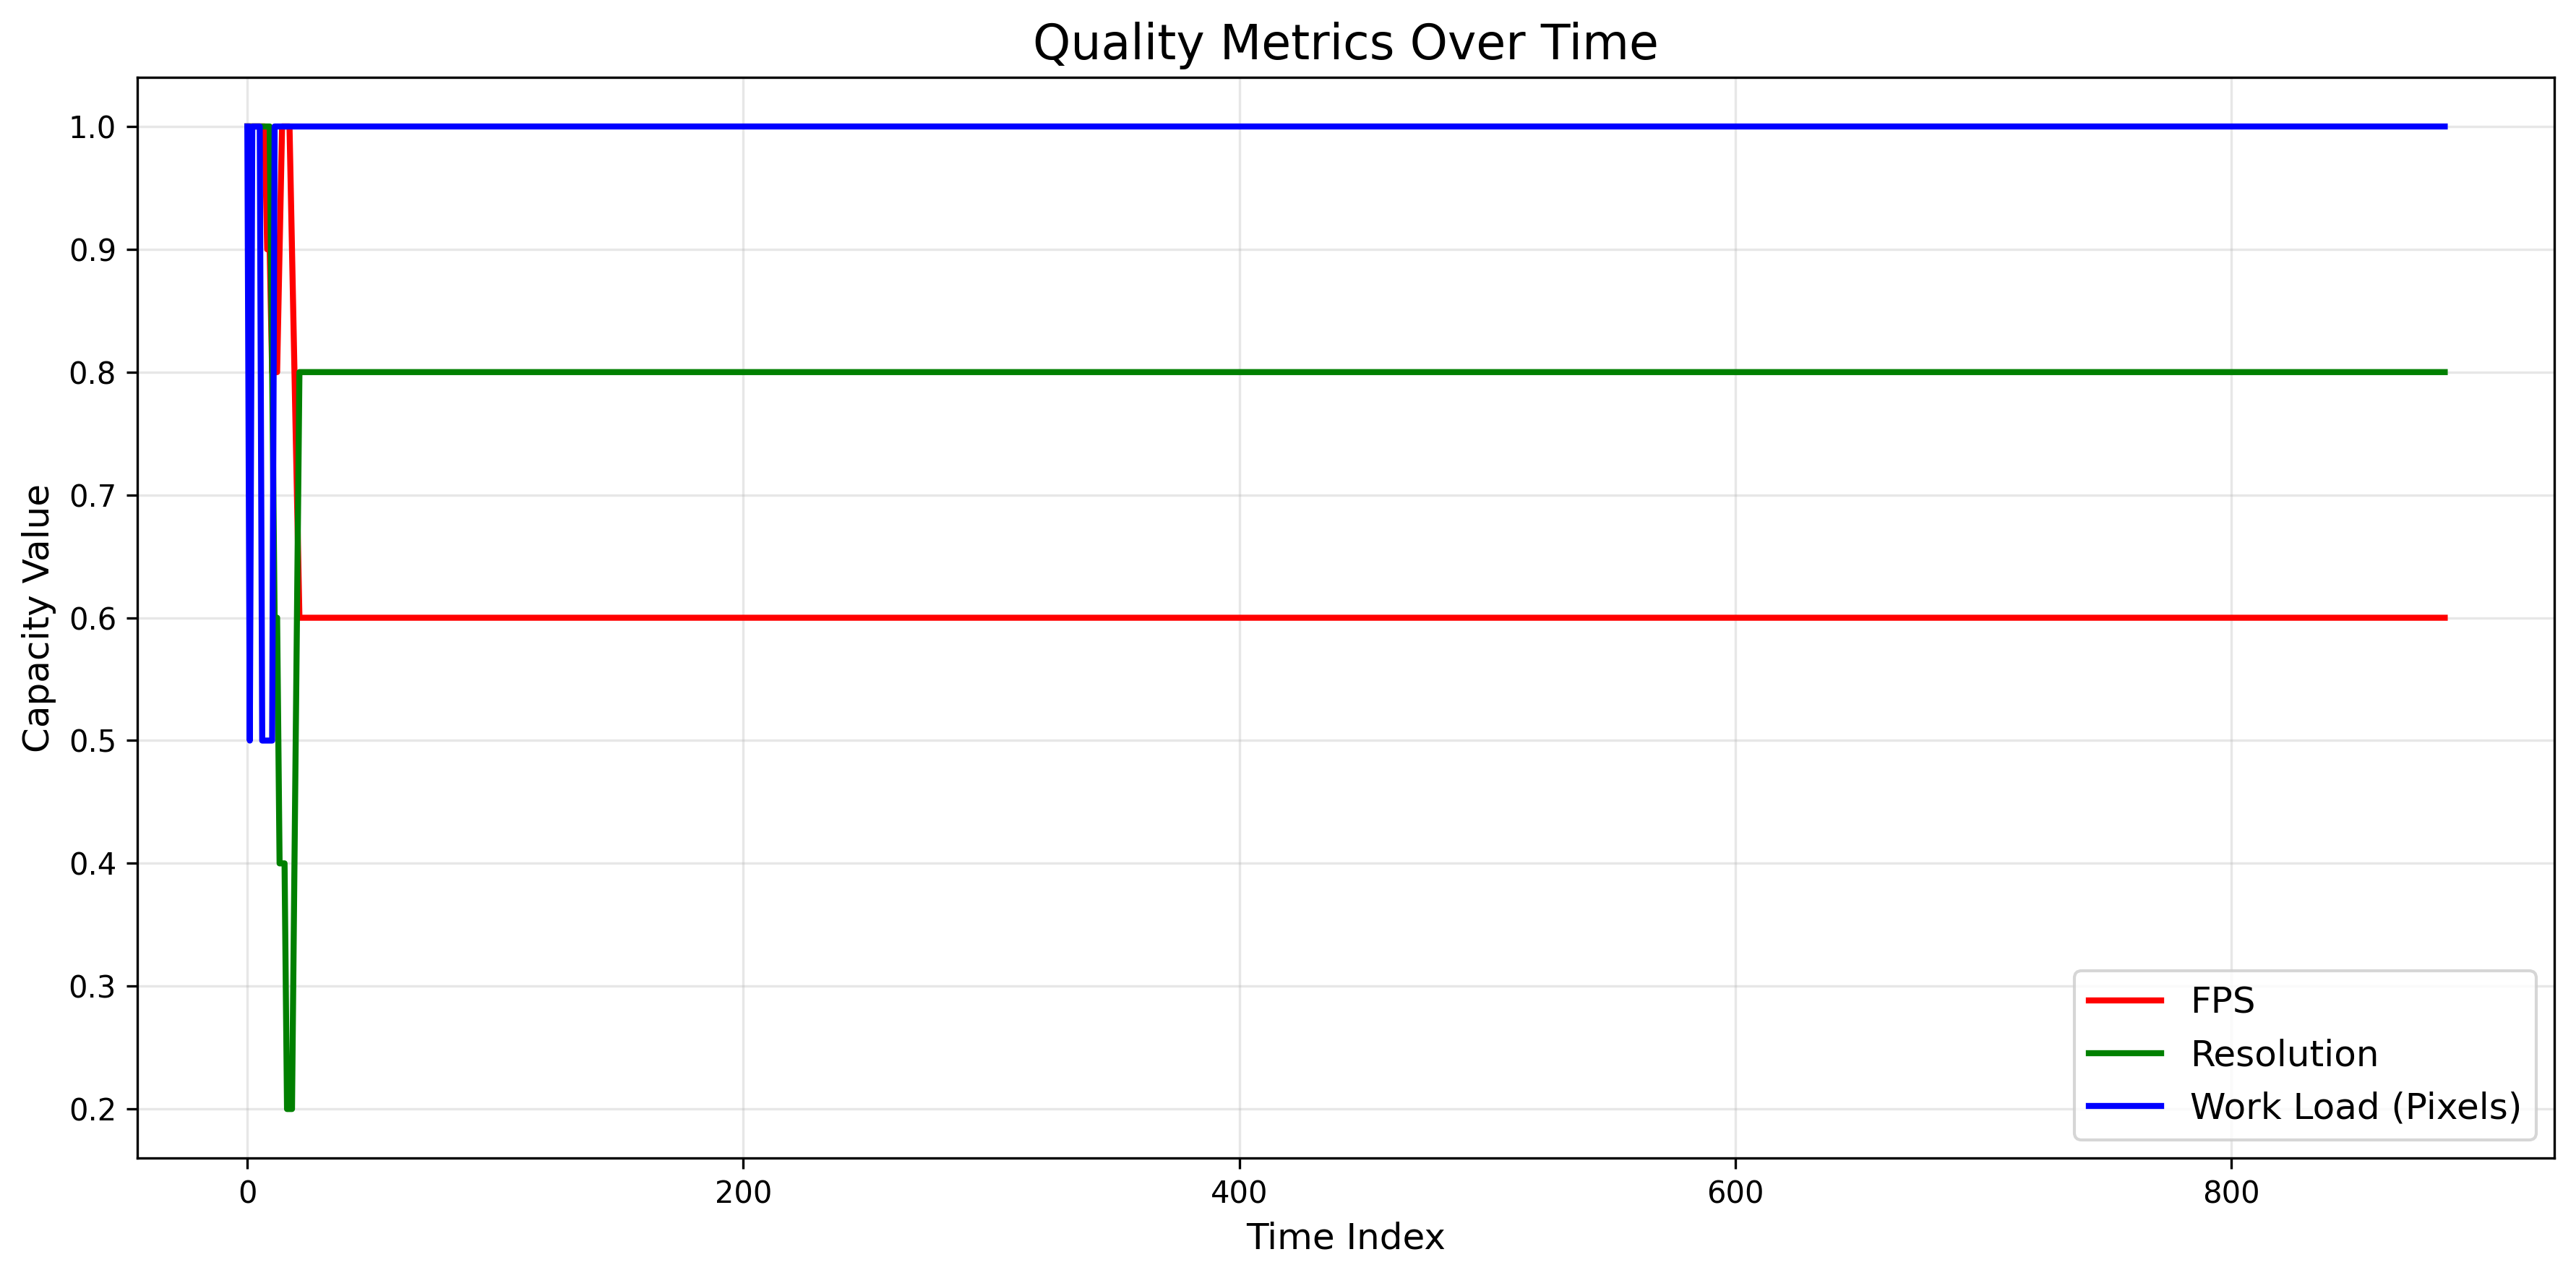
\includegraphics[width=\textwidth]{img/results/basic_sim/active_inference_relative_control_quality_metrics.png}
    \caption{AIF – Quality Metrics Over Time (Base Case)}
\end{figure}

\begin{figure}[h]
    \centering
    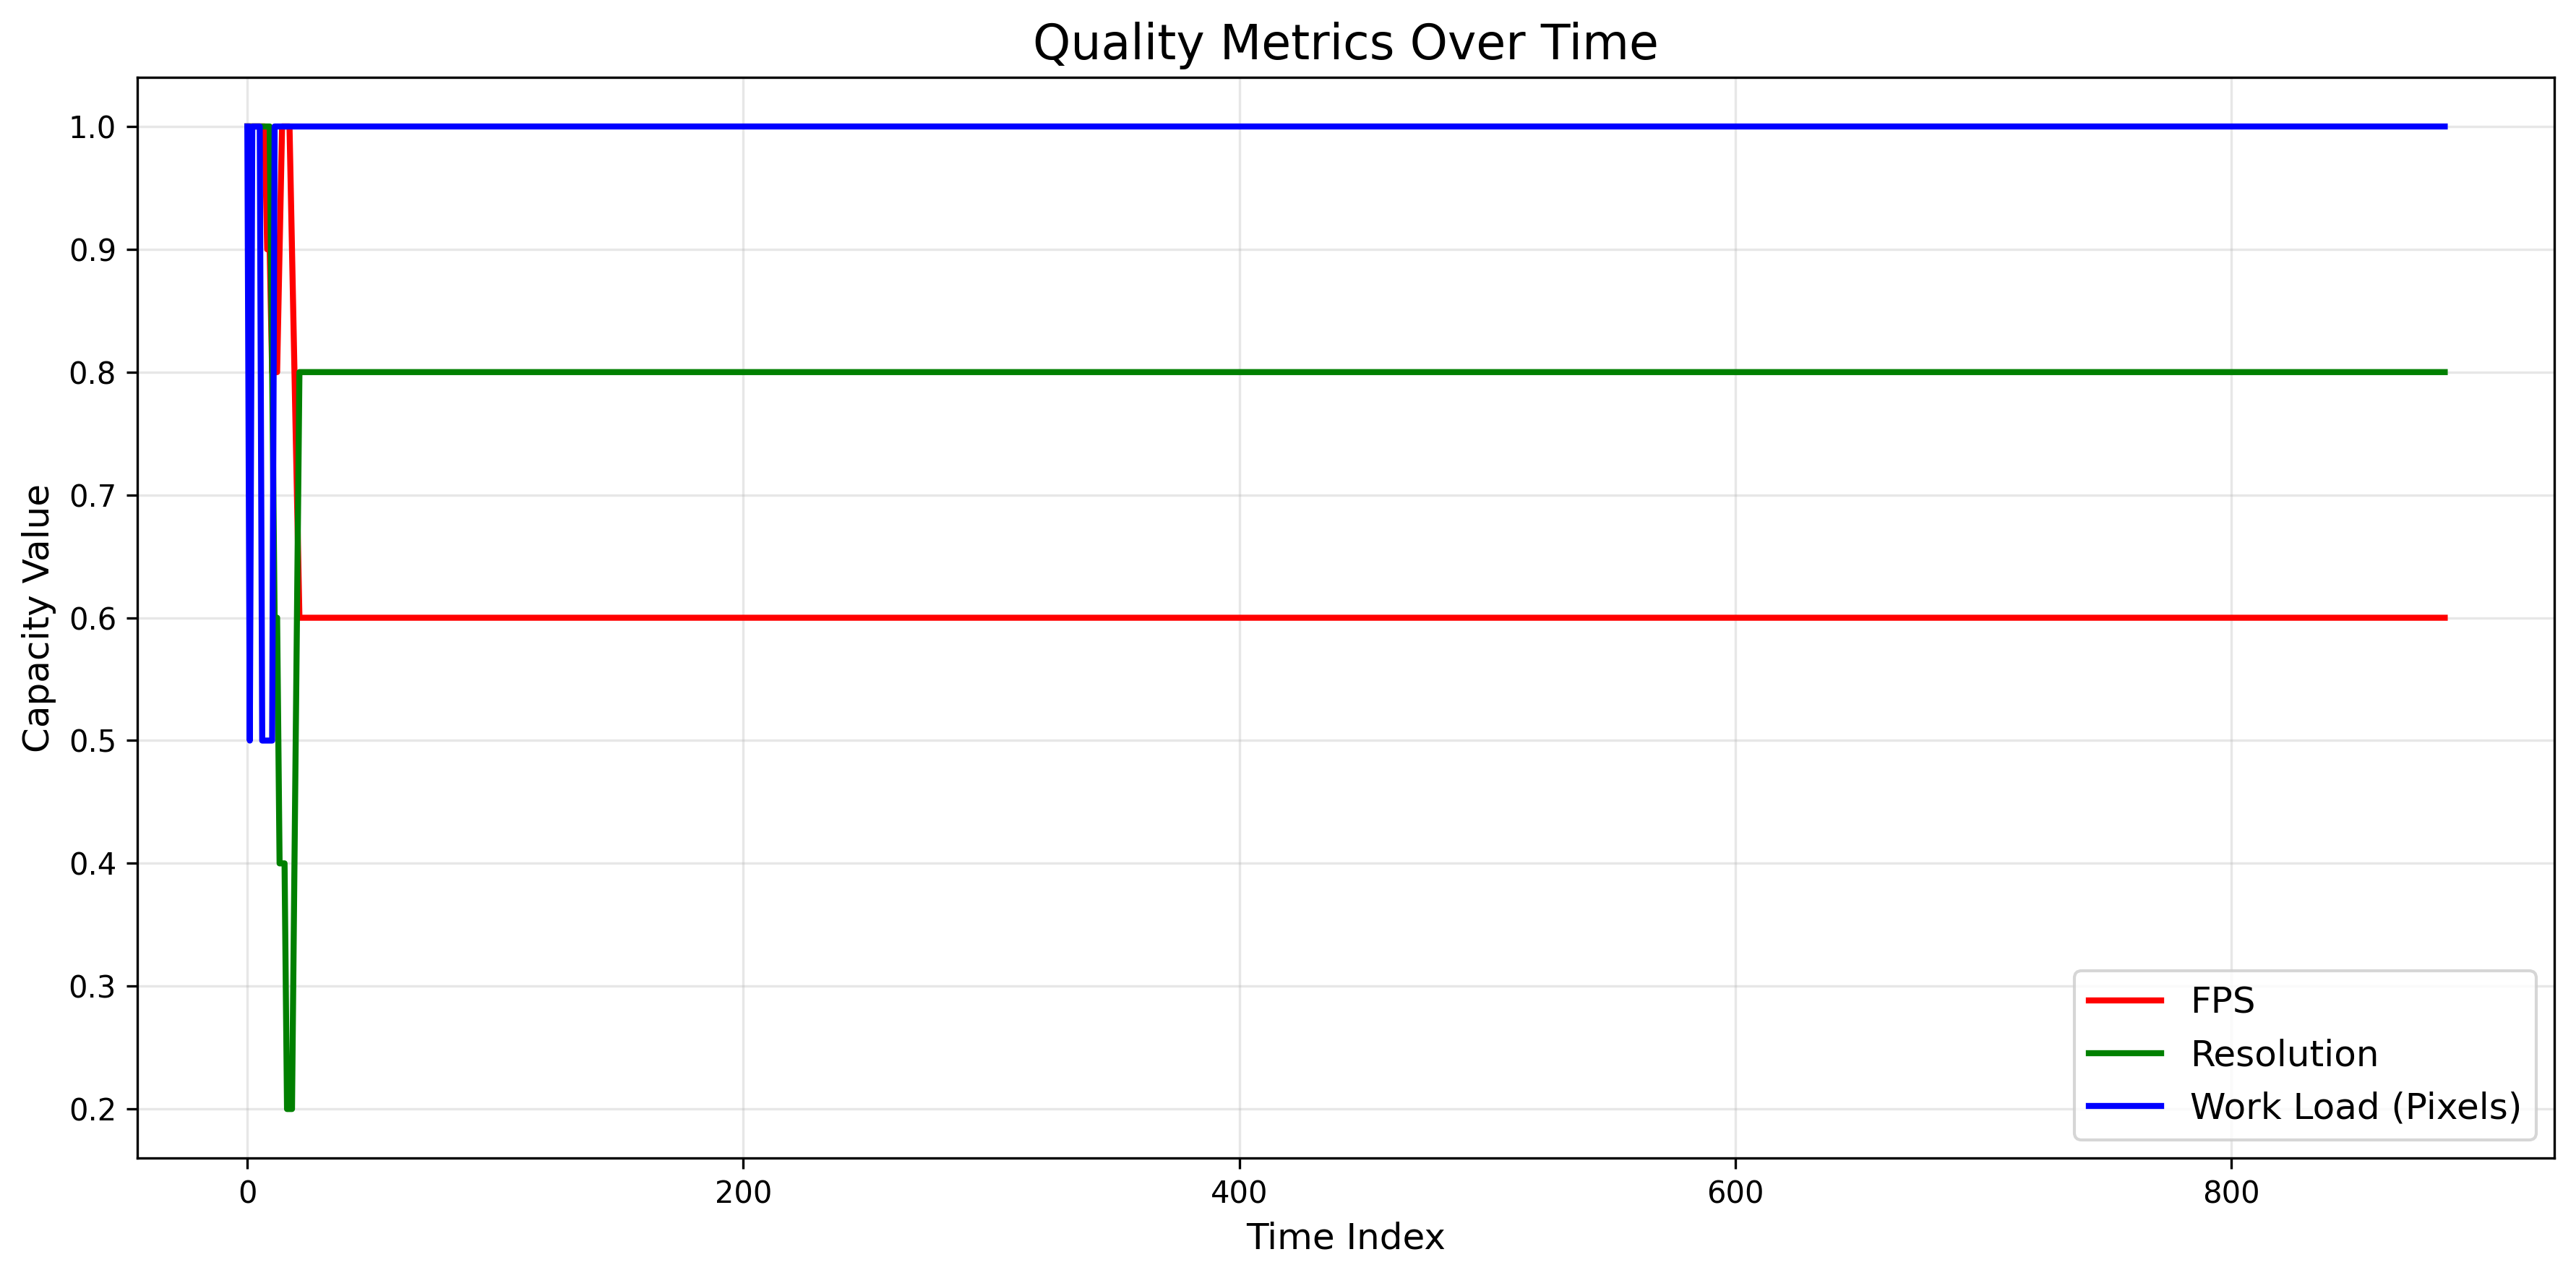
\includegraphics[width=\textwidth]{img/results/basic_sim/active_inference_relative_control_quality_metrics.png}
    \caption{AIF – Quality Metrics Over Time (Base Case)}
\end{figure}
\begin{figure}[h]
    \centering
    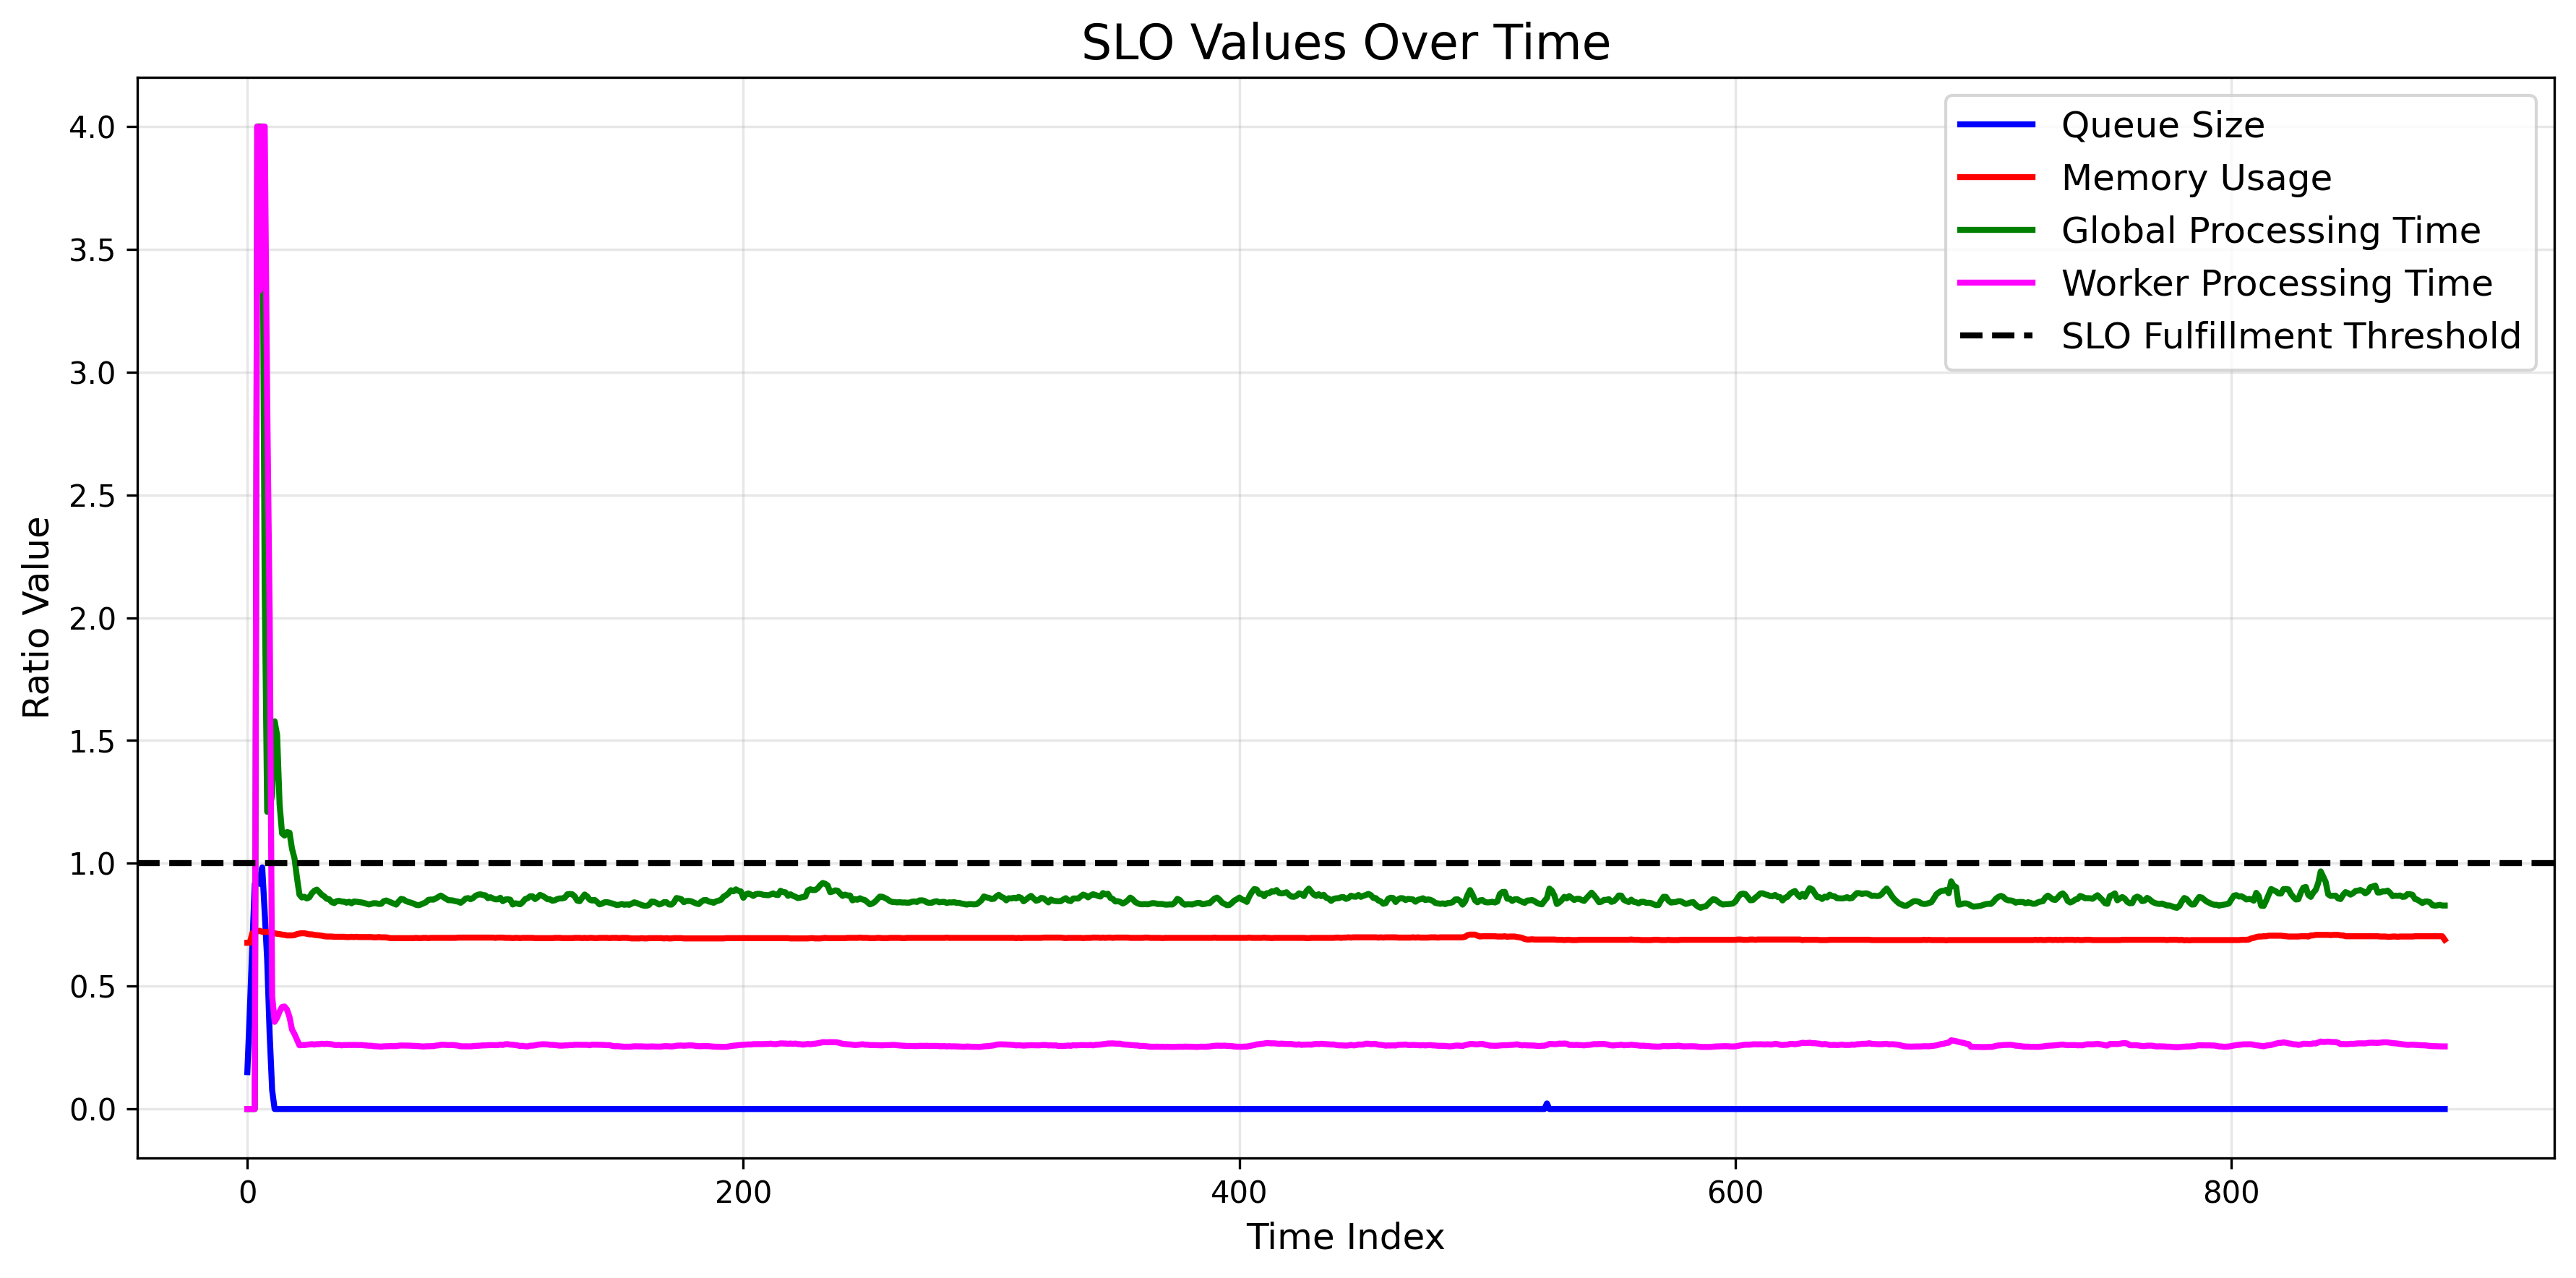
\includegraphics[width=\textwidth]{img/results/basic_sim/active_inference_relative_control_slo_values.png}
    \caption{AIF – SLO Metrics Over Time (Base Case)}
\end{figure}
\begin{figure}[h]
    \centering
    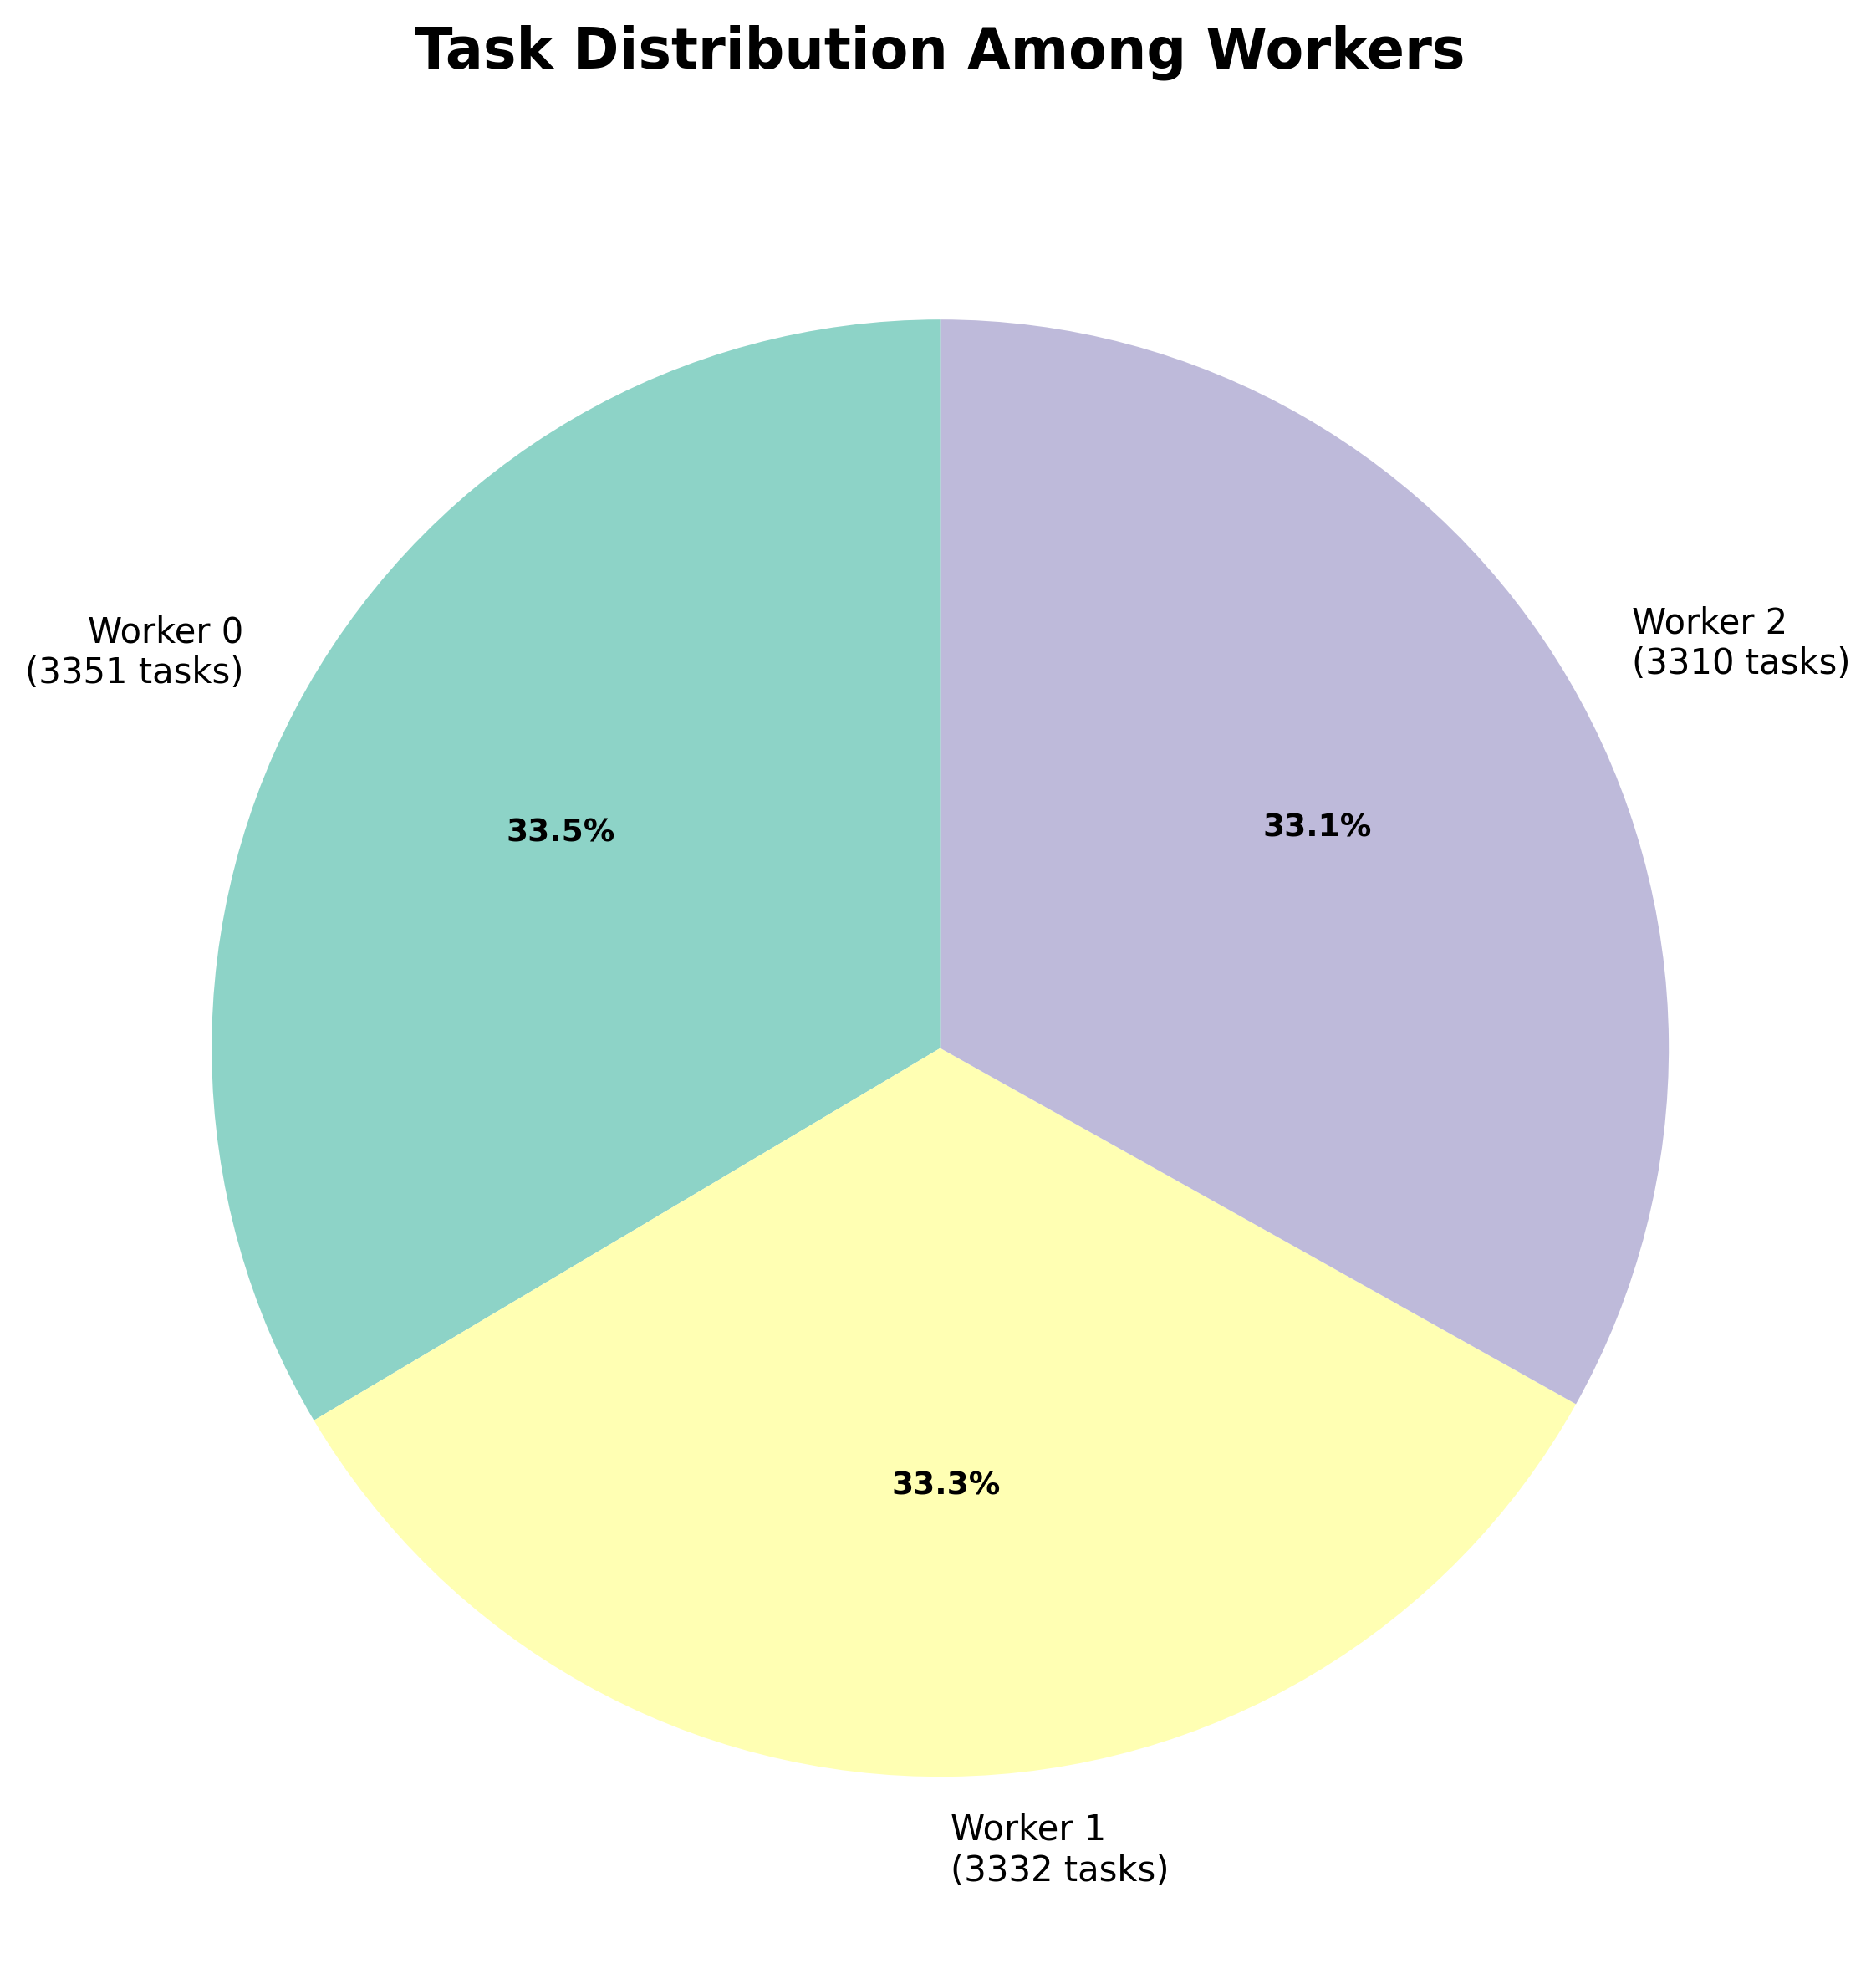
\includegraphics[width=0.5\textwidth]{img/results/basic_sim/active_inference_relative_control_task_distribution_pie.png}
    \caption{AIF – Task Distribution (Base Case)}
\end{figure}
\begin{figure}[h]
    \centering
    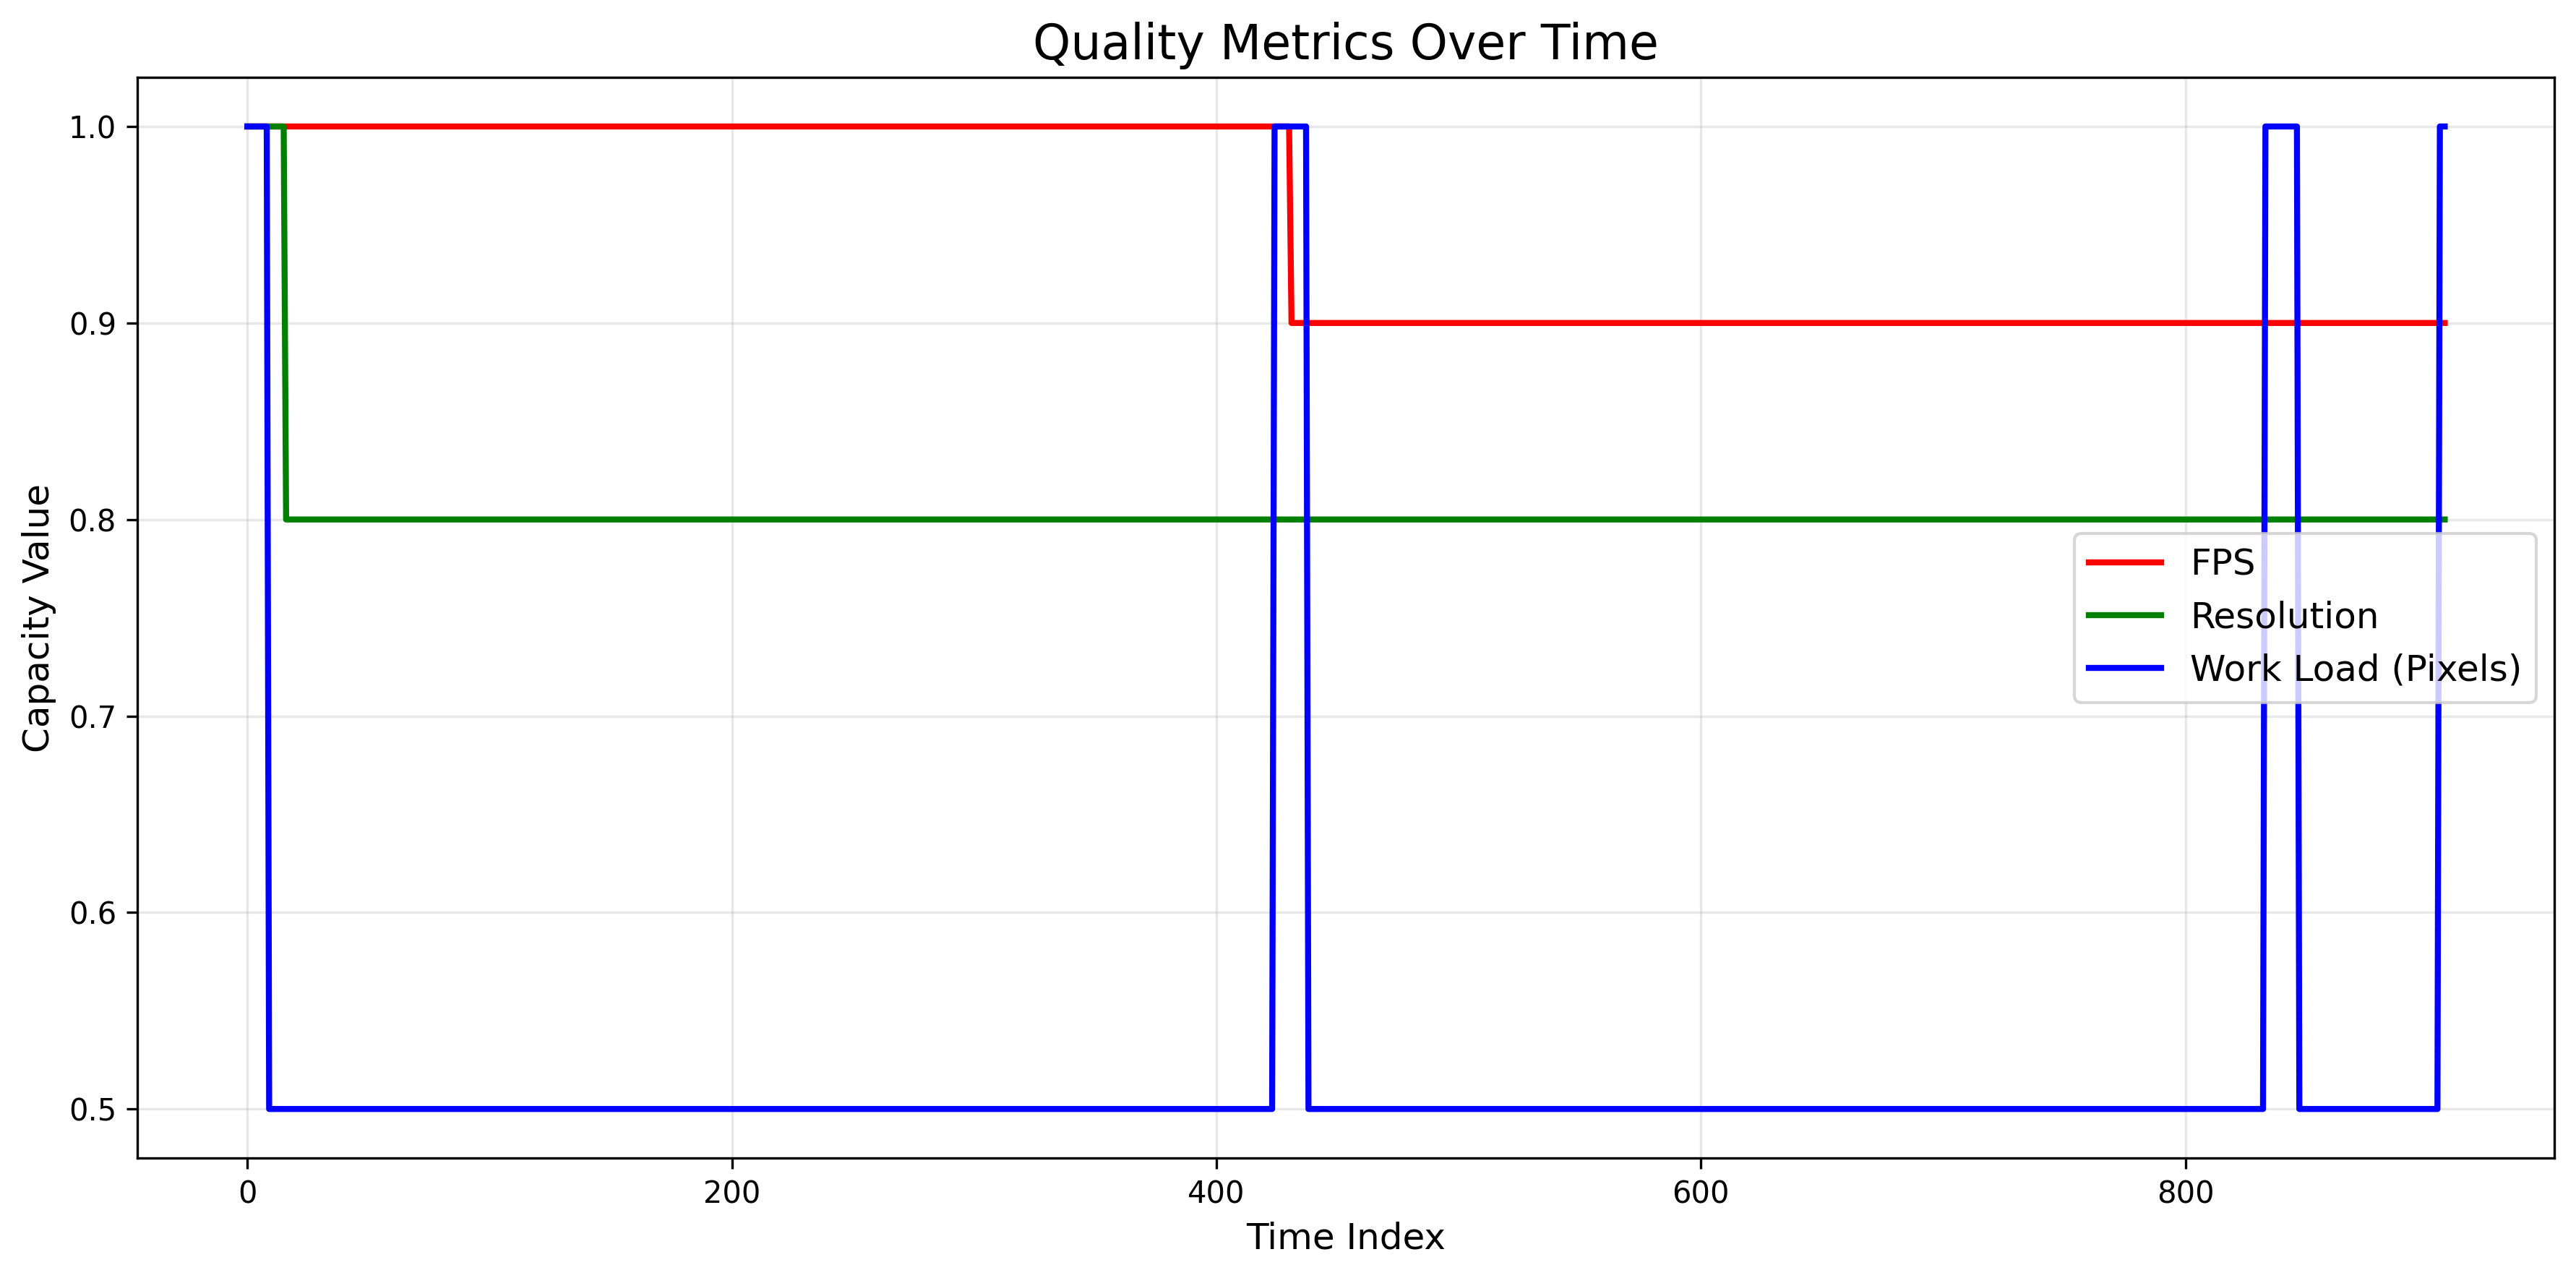
\includegraphics[width=\textwidth]{img/results/basic_sim/heuristic_quality_metrics.png}
    \caption{Heuristic – Quality Metrics Over Time (Base Case)}
\end{figure}
\begin{figure}[h]
    \centering
    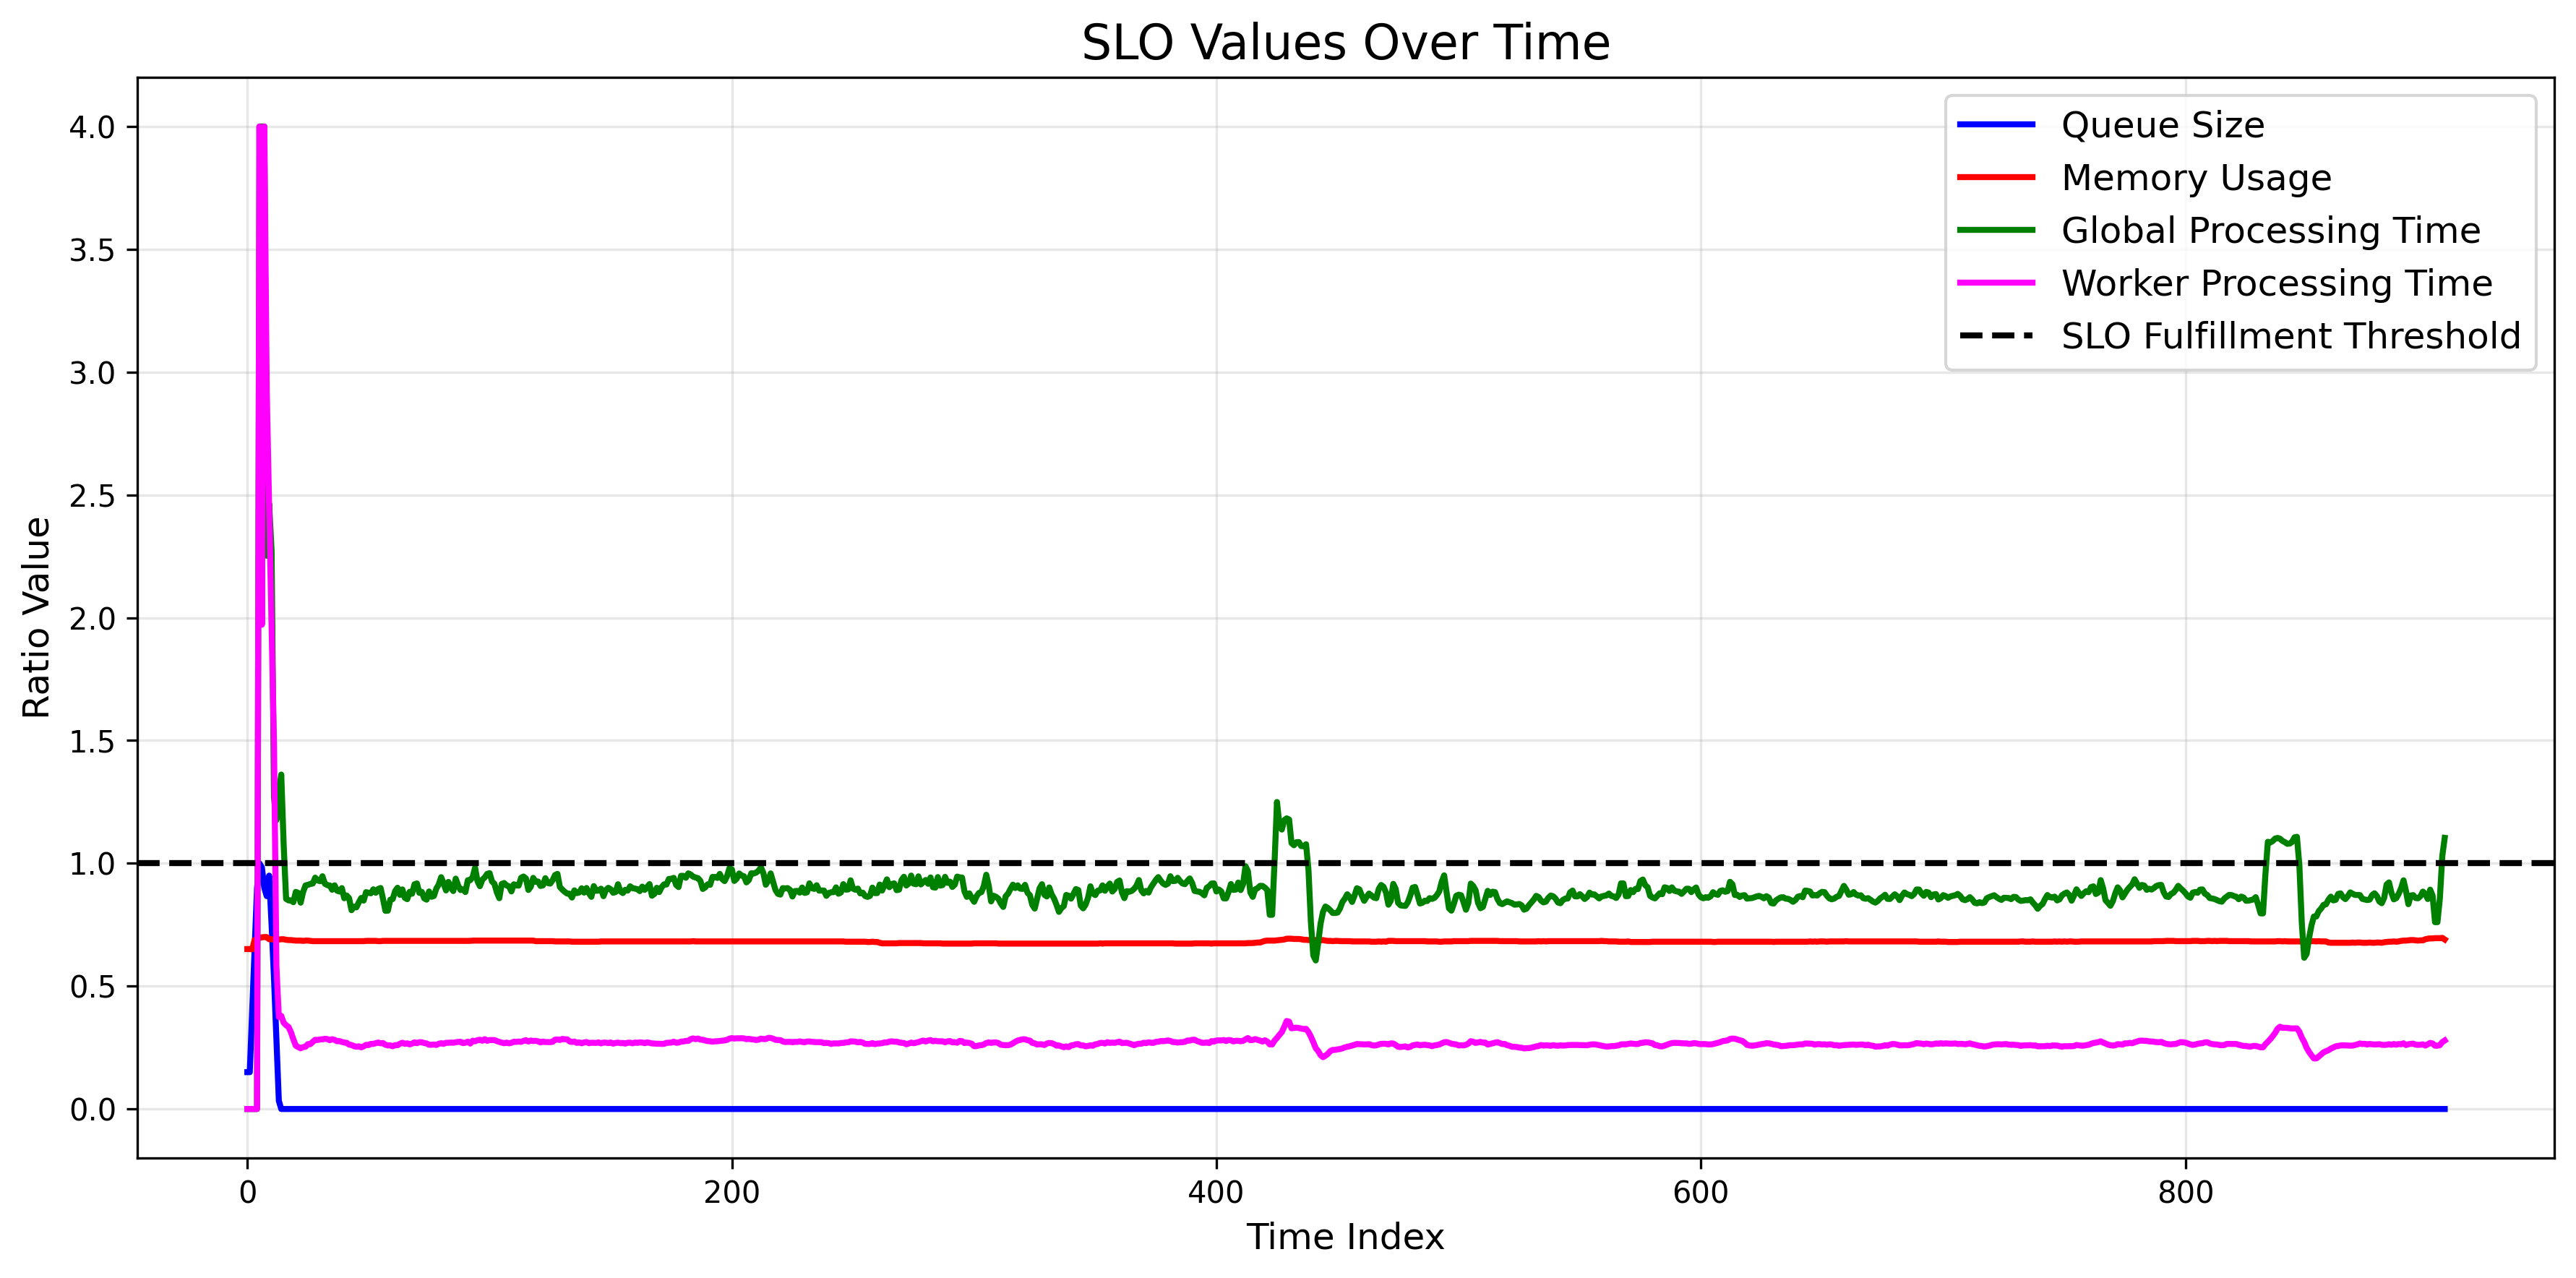
\includegraphics[width=\textwidth]{img/results/basic_sim/heuristic_slo_values.png}
    \caption{Heuristic – SLO Metrics Over Time (Base Case)}
\end{figure}
\begin{figure}[h]
    \centering
    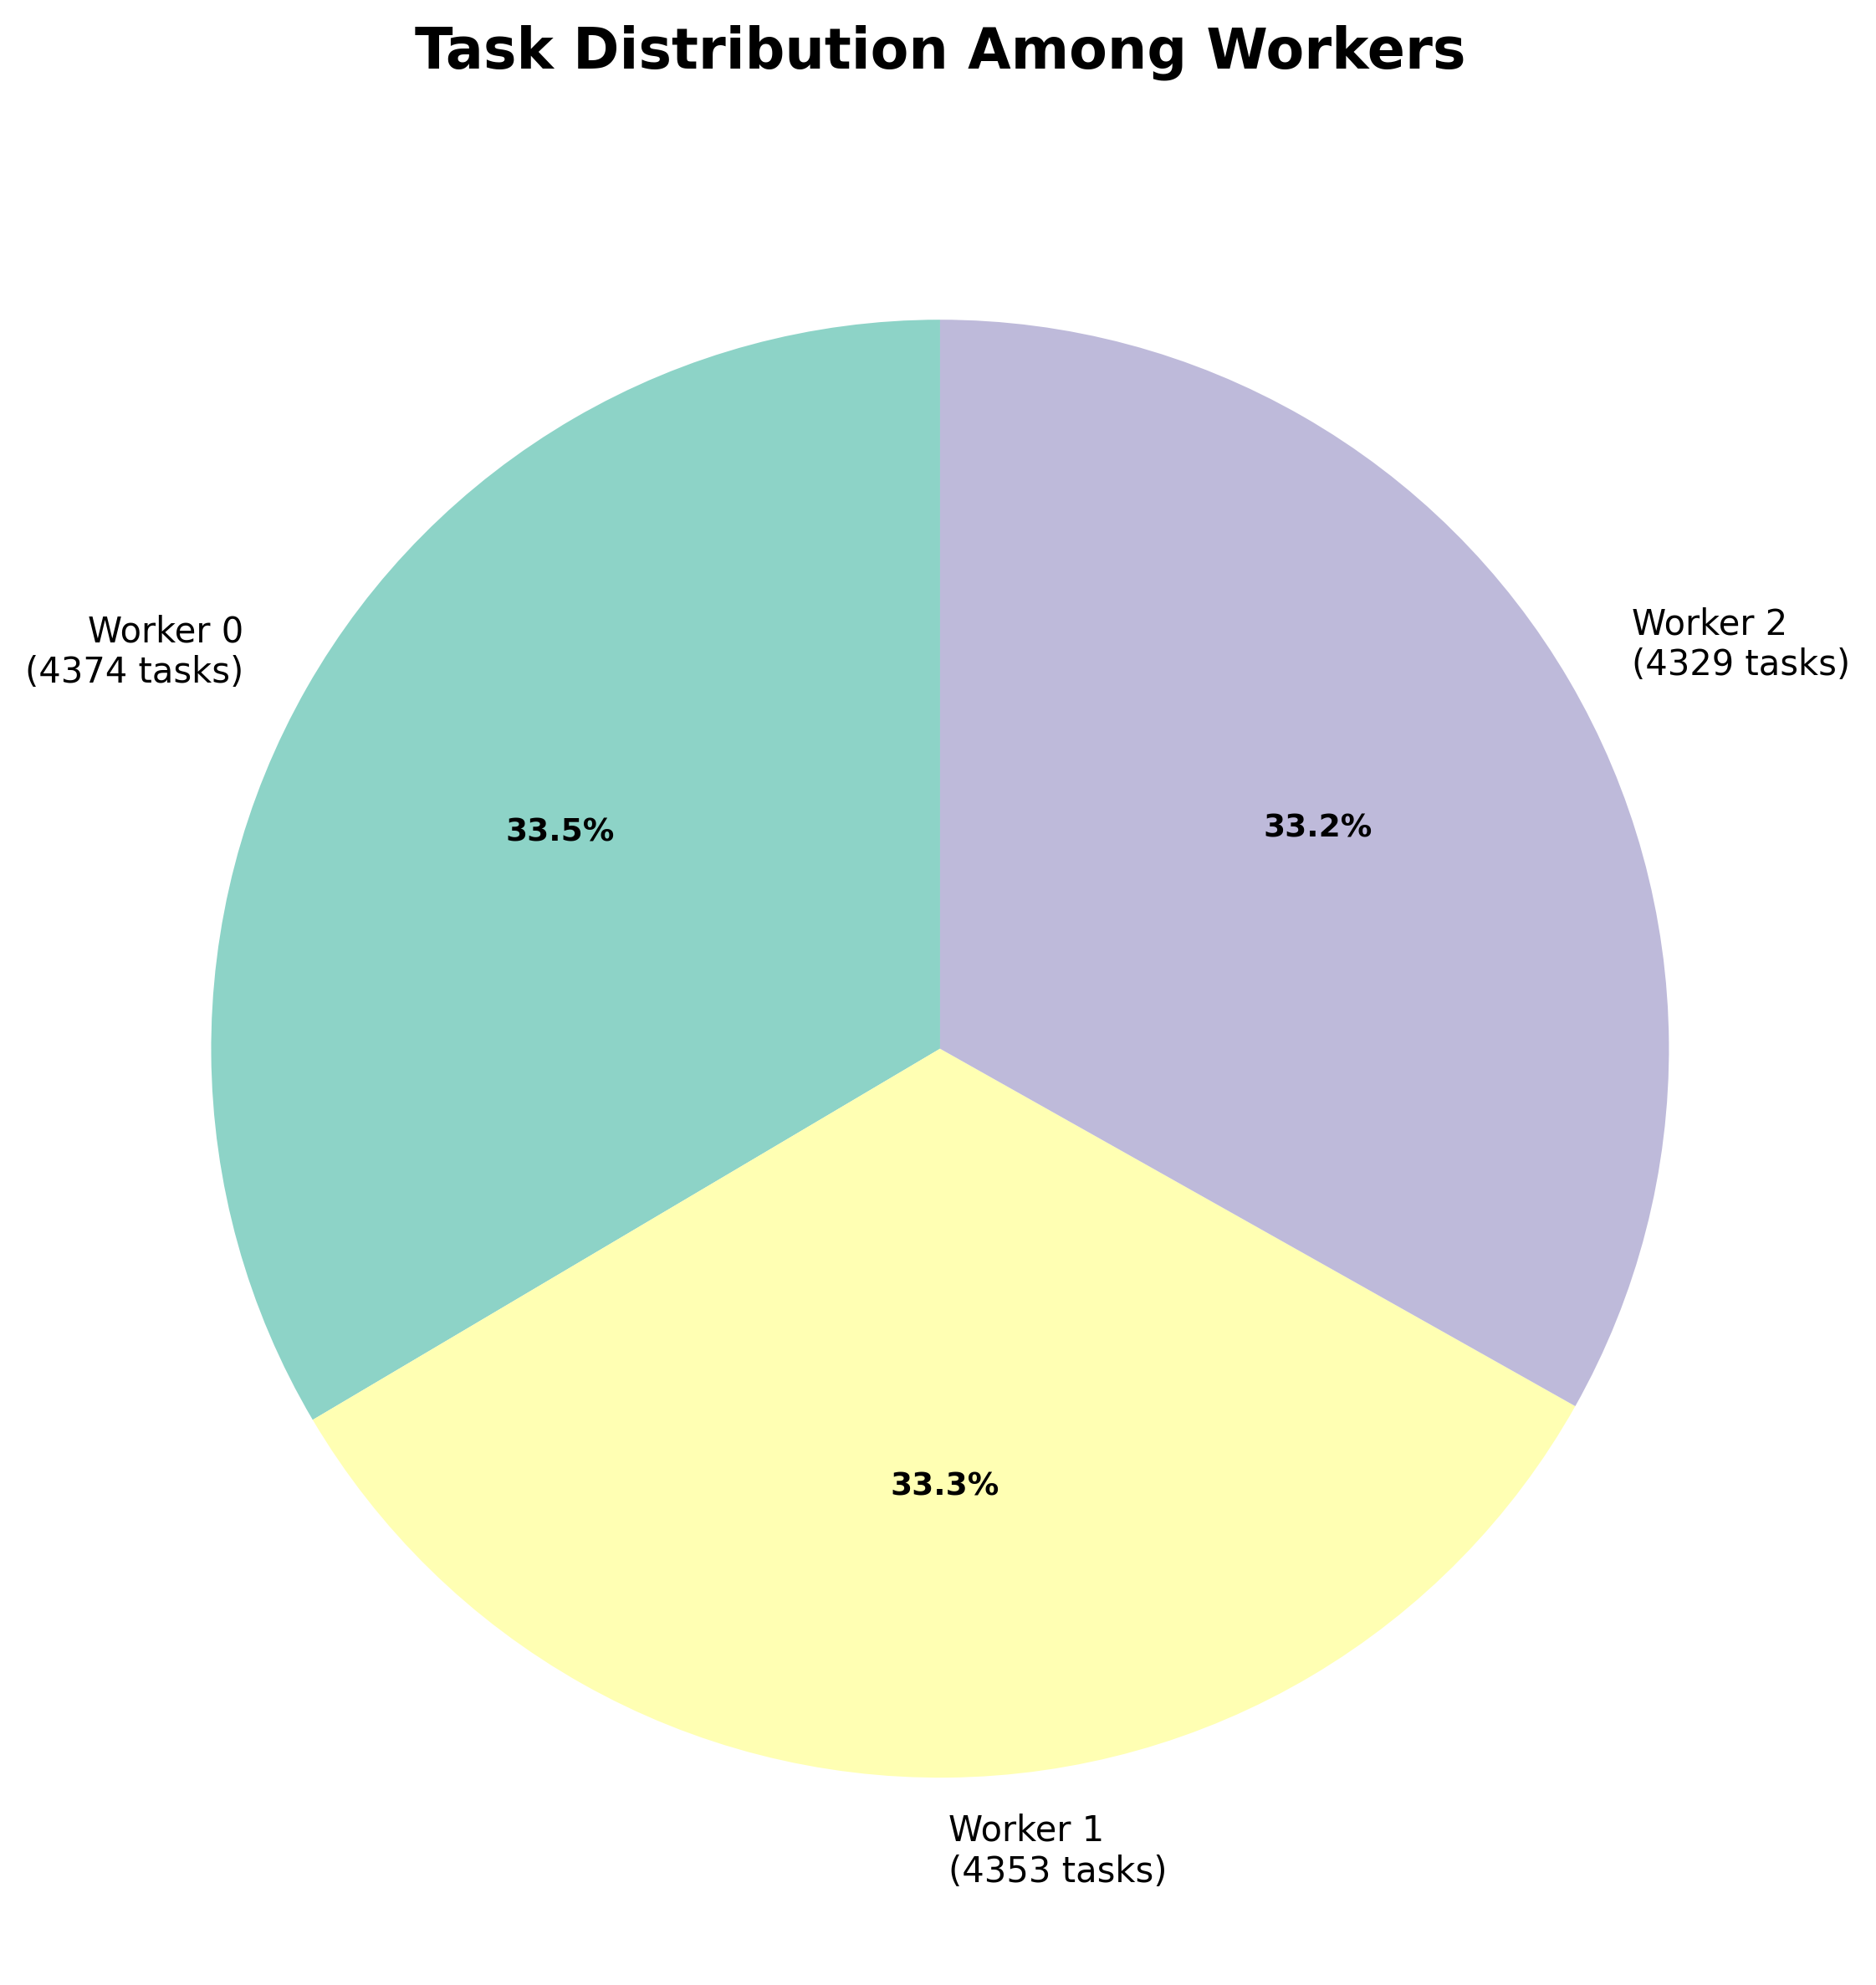
\includegraphics[width=0.5\textwidth]{img/results/basic_sim/heuristic_task_distribution_pie.png}
    \caption{Heuristic – Task Distribution (Base Case)}
\end{figure}

\clearpage
\section{Scenario B: Variable Computational Demand}

\subsection*{Active Inference Agent}
\begin{table}[h]
\centering
\caption{Demand – Active Inference}
\label{tab:demand_active_inference}
\begin{tabular}{lr}
\toprule
Metric & Value \\
\midrule
Total Simulation Timesteps & 922 \\
\% Time All SLOs Met & 0.7126 \\
Average SLO Fulfillment Rate & 0.9073 \\
Average Overall Stream Quality Score & 0.7663 \\
Max Consecutive SLO Violations & 259 \\
Time to Reach Stable Configuration & 1.0000 \\
Queue Size SLO Fulfillment Rate & 0.7191 \\
Memory Usage SLO Fulfillment Rate & 1.0000 \\
Global Processing Time SLO Fulfillment Rate & 0.9154 \\
Worker Processing Time SLO Fulfillment Rate & 0.9946 \\
Queue Size Violation Severity (Avg) & 1.3123 \\
Worker Proc. Time Violation Severity (Avg) & 1.9074 \\
\bottomrule
\end{tabular}
\end{table}


\subsection*{Heuristic Agent}
\begin{table}[h]
\centering
\caption{Demand – Heuristic}
\label{tab:demand_heuristic}
\begin{tabular}{lr}
\toprule
Metric & Value \\
\midrule
Total Simulation Timesteps & 992 \\
\% Time All SLOs Met & 0.8518 \\
Average SLO Fulfillment Rate & 0.9488 \\
Average Overall Stream Quality Score & 0.8216 \\
Max Consecutive SLO Violations & 68 \\
Time to Reach Stable Configuration & 0.9697 \\
Queue Size SLO Fulfillment Rate & 0.8821 \\
Memory Usage SLO Fulfillment Rate & 1.0000 \\
Global Processing Time SLO Fulfillment Rate & 0.9163 \\
Worker Processing Time SLO Fulfillment Rate & 0.9970 \\
Queue Size Violation Severity (Avg) & 0.9526 \\
Worker Proc. Time Violation Severity (Avg) & 0.5446 \\
\bottomrule
\end{tabular}
\end{table}


\subsection*{Plots}
\begin{figure}[h]
    \centering
    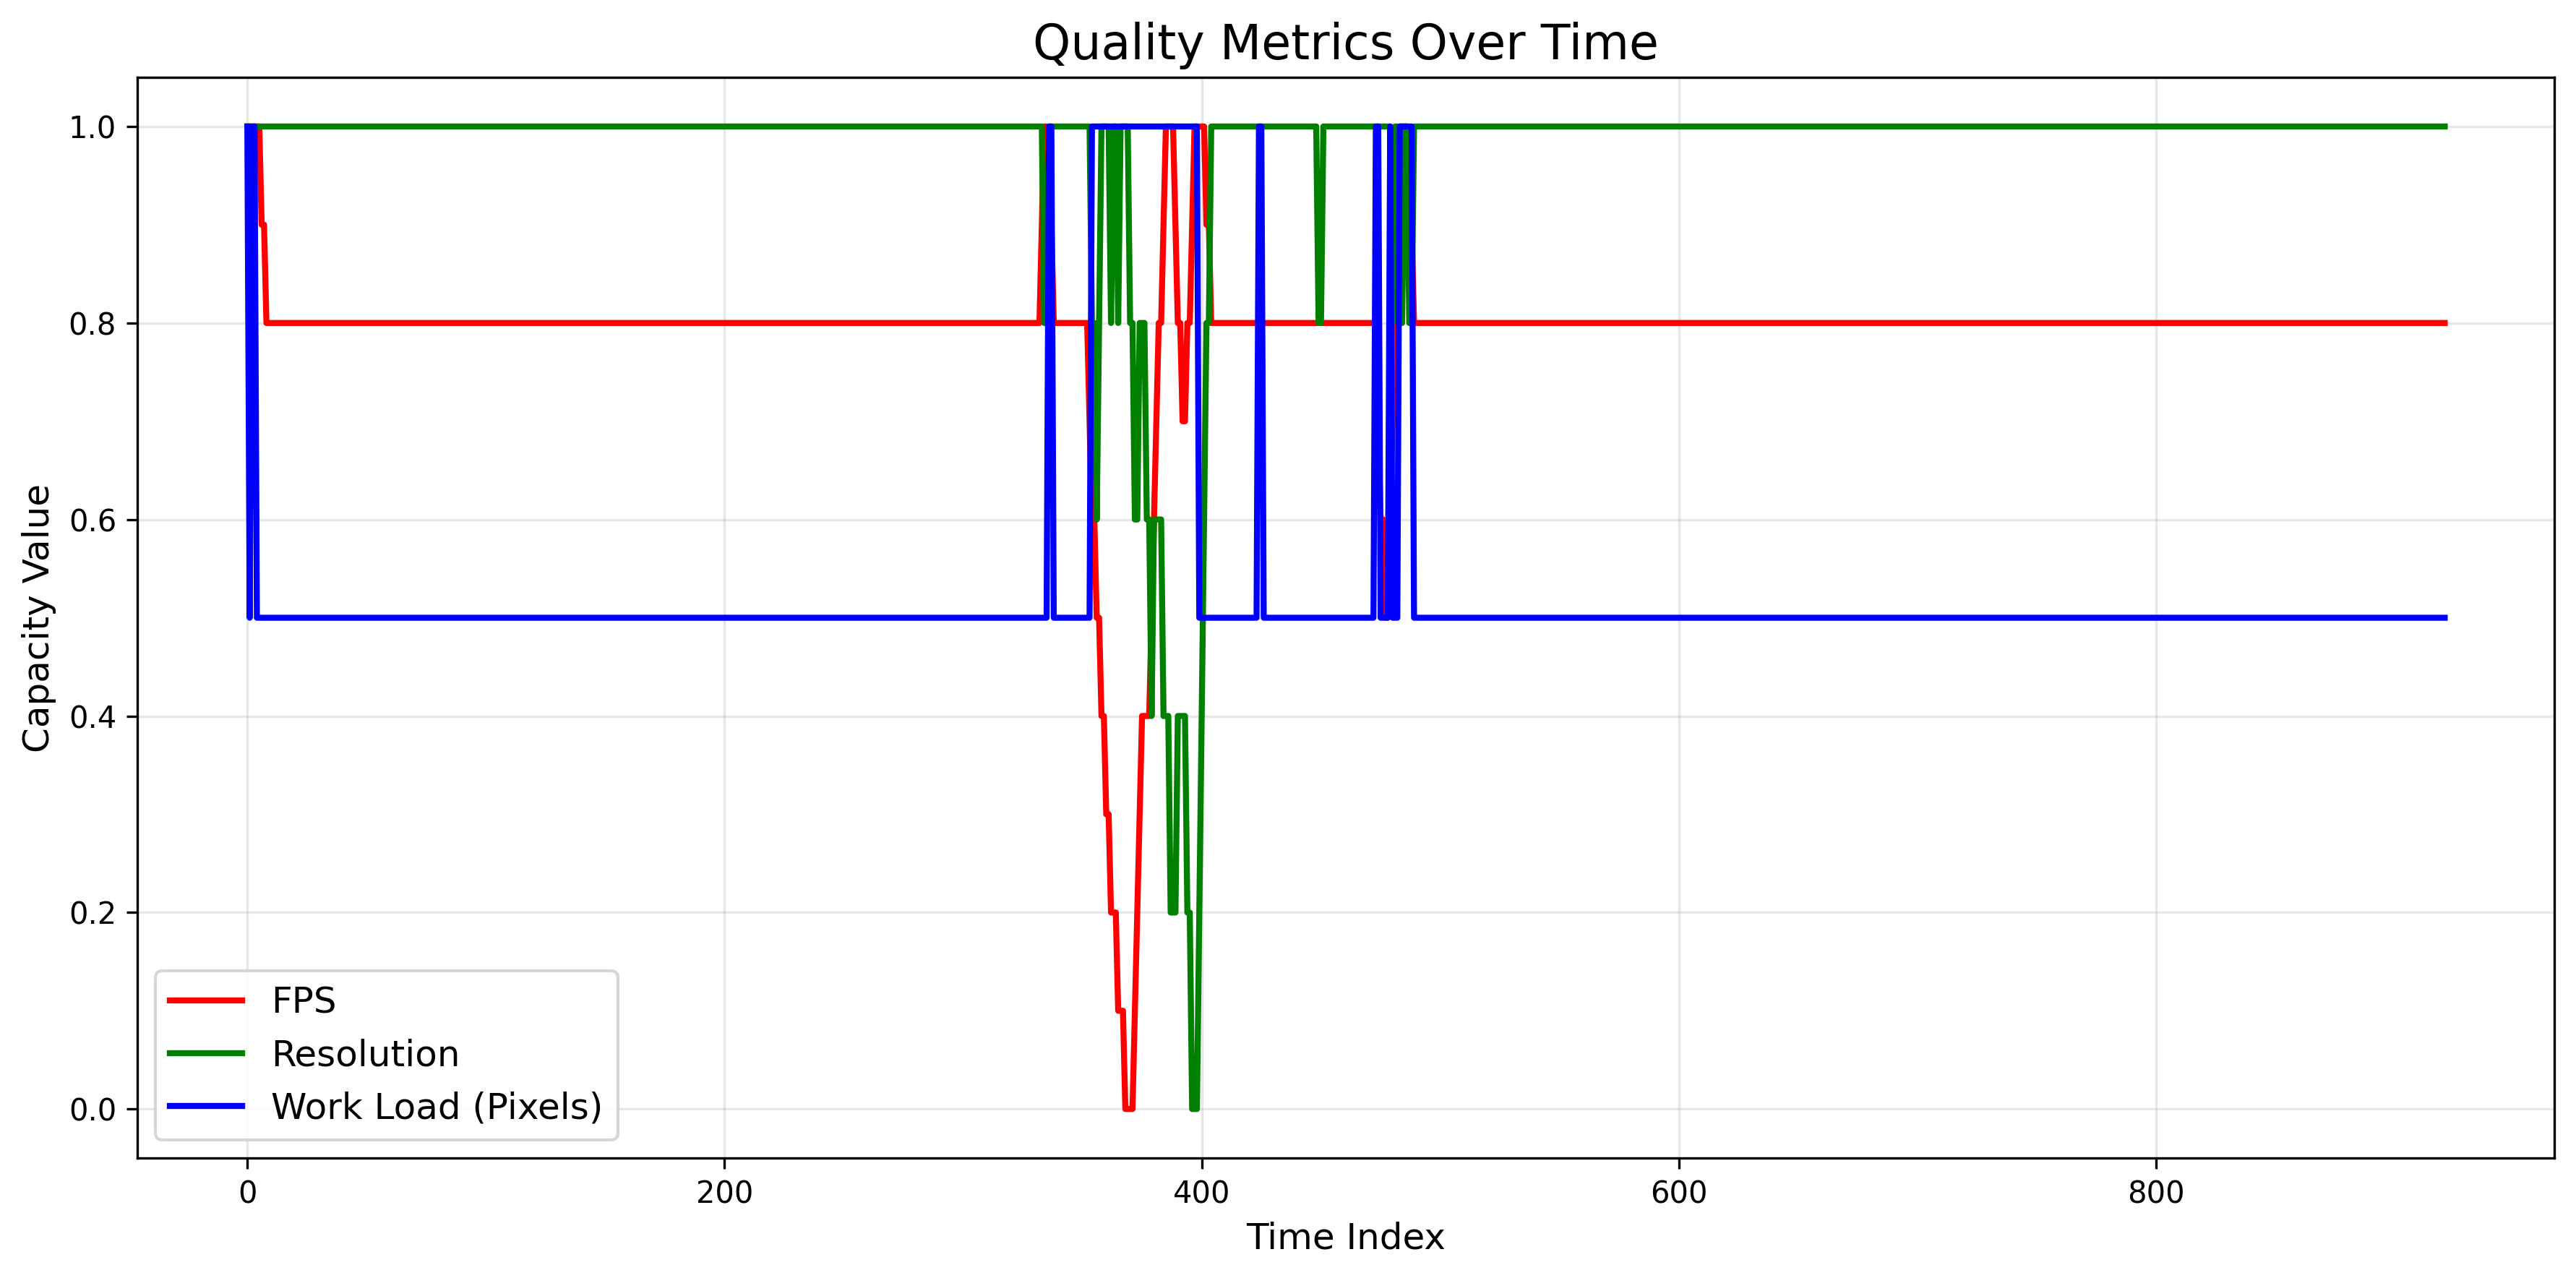
\includegraphics[width=\textwidth]{img/results/variable_computational_demand_sim/active_inference_relative_control_quality_metrics.png}
    \caption{AIF – Quality Metrics Over Time (Demand)}
\end{figure}
\begin{figure}[h]
    \centering
    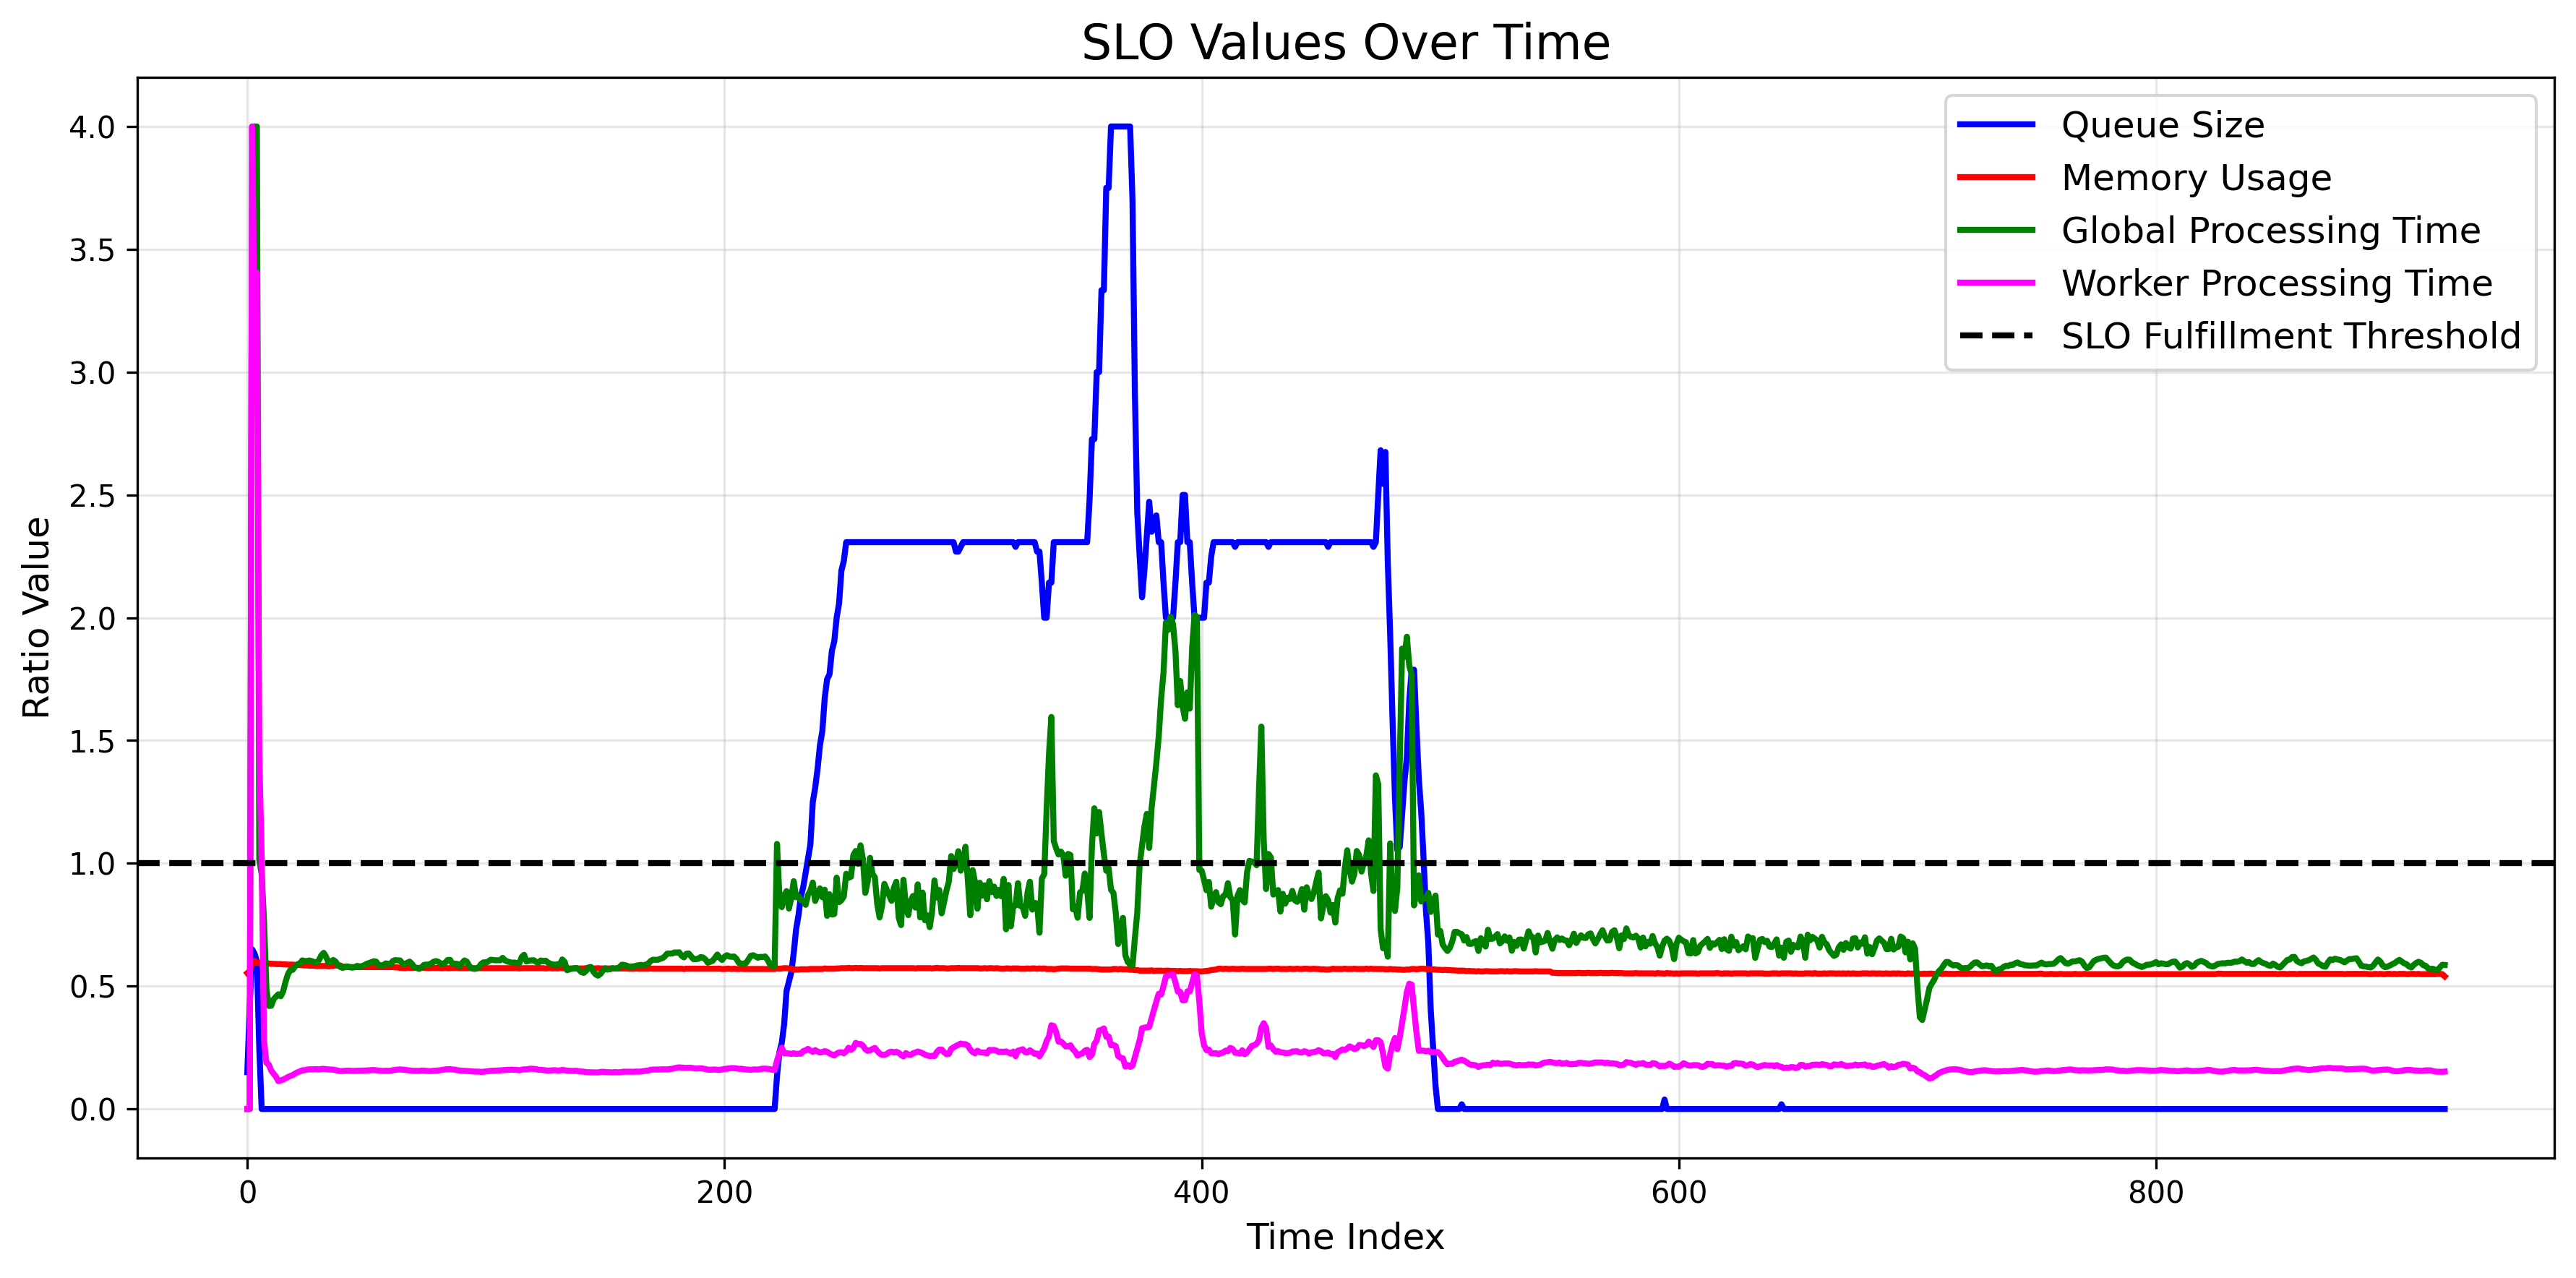
\includegraphics[width=\textwidth]{img/results/variable_computational_demand_sim/active_inference_relative_control_slo_values.png}
    \caption{AIF – SLO Metrics Over Time (Demand)}
\end{figure}
\begin{figure}[h]
    \centering
    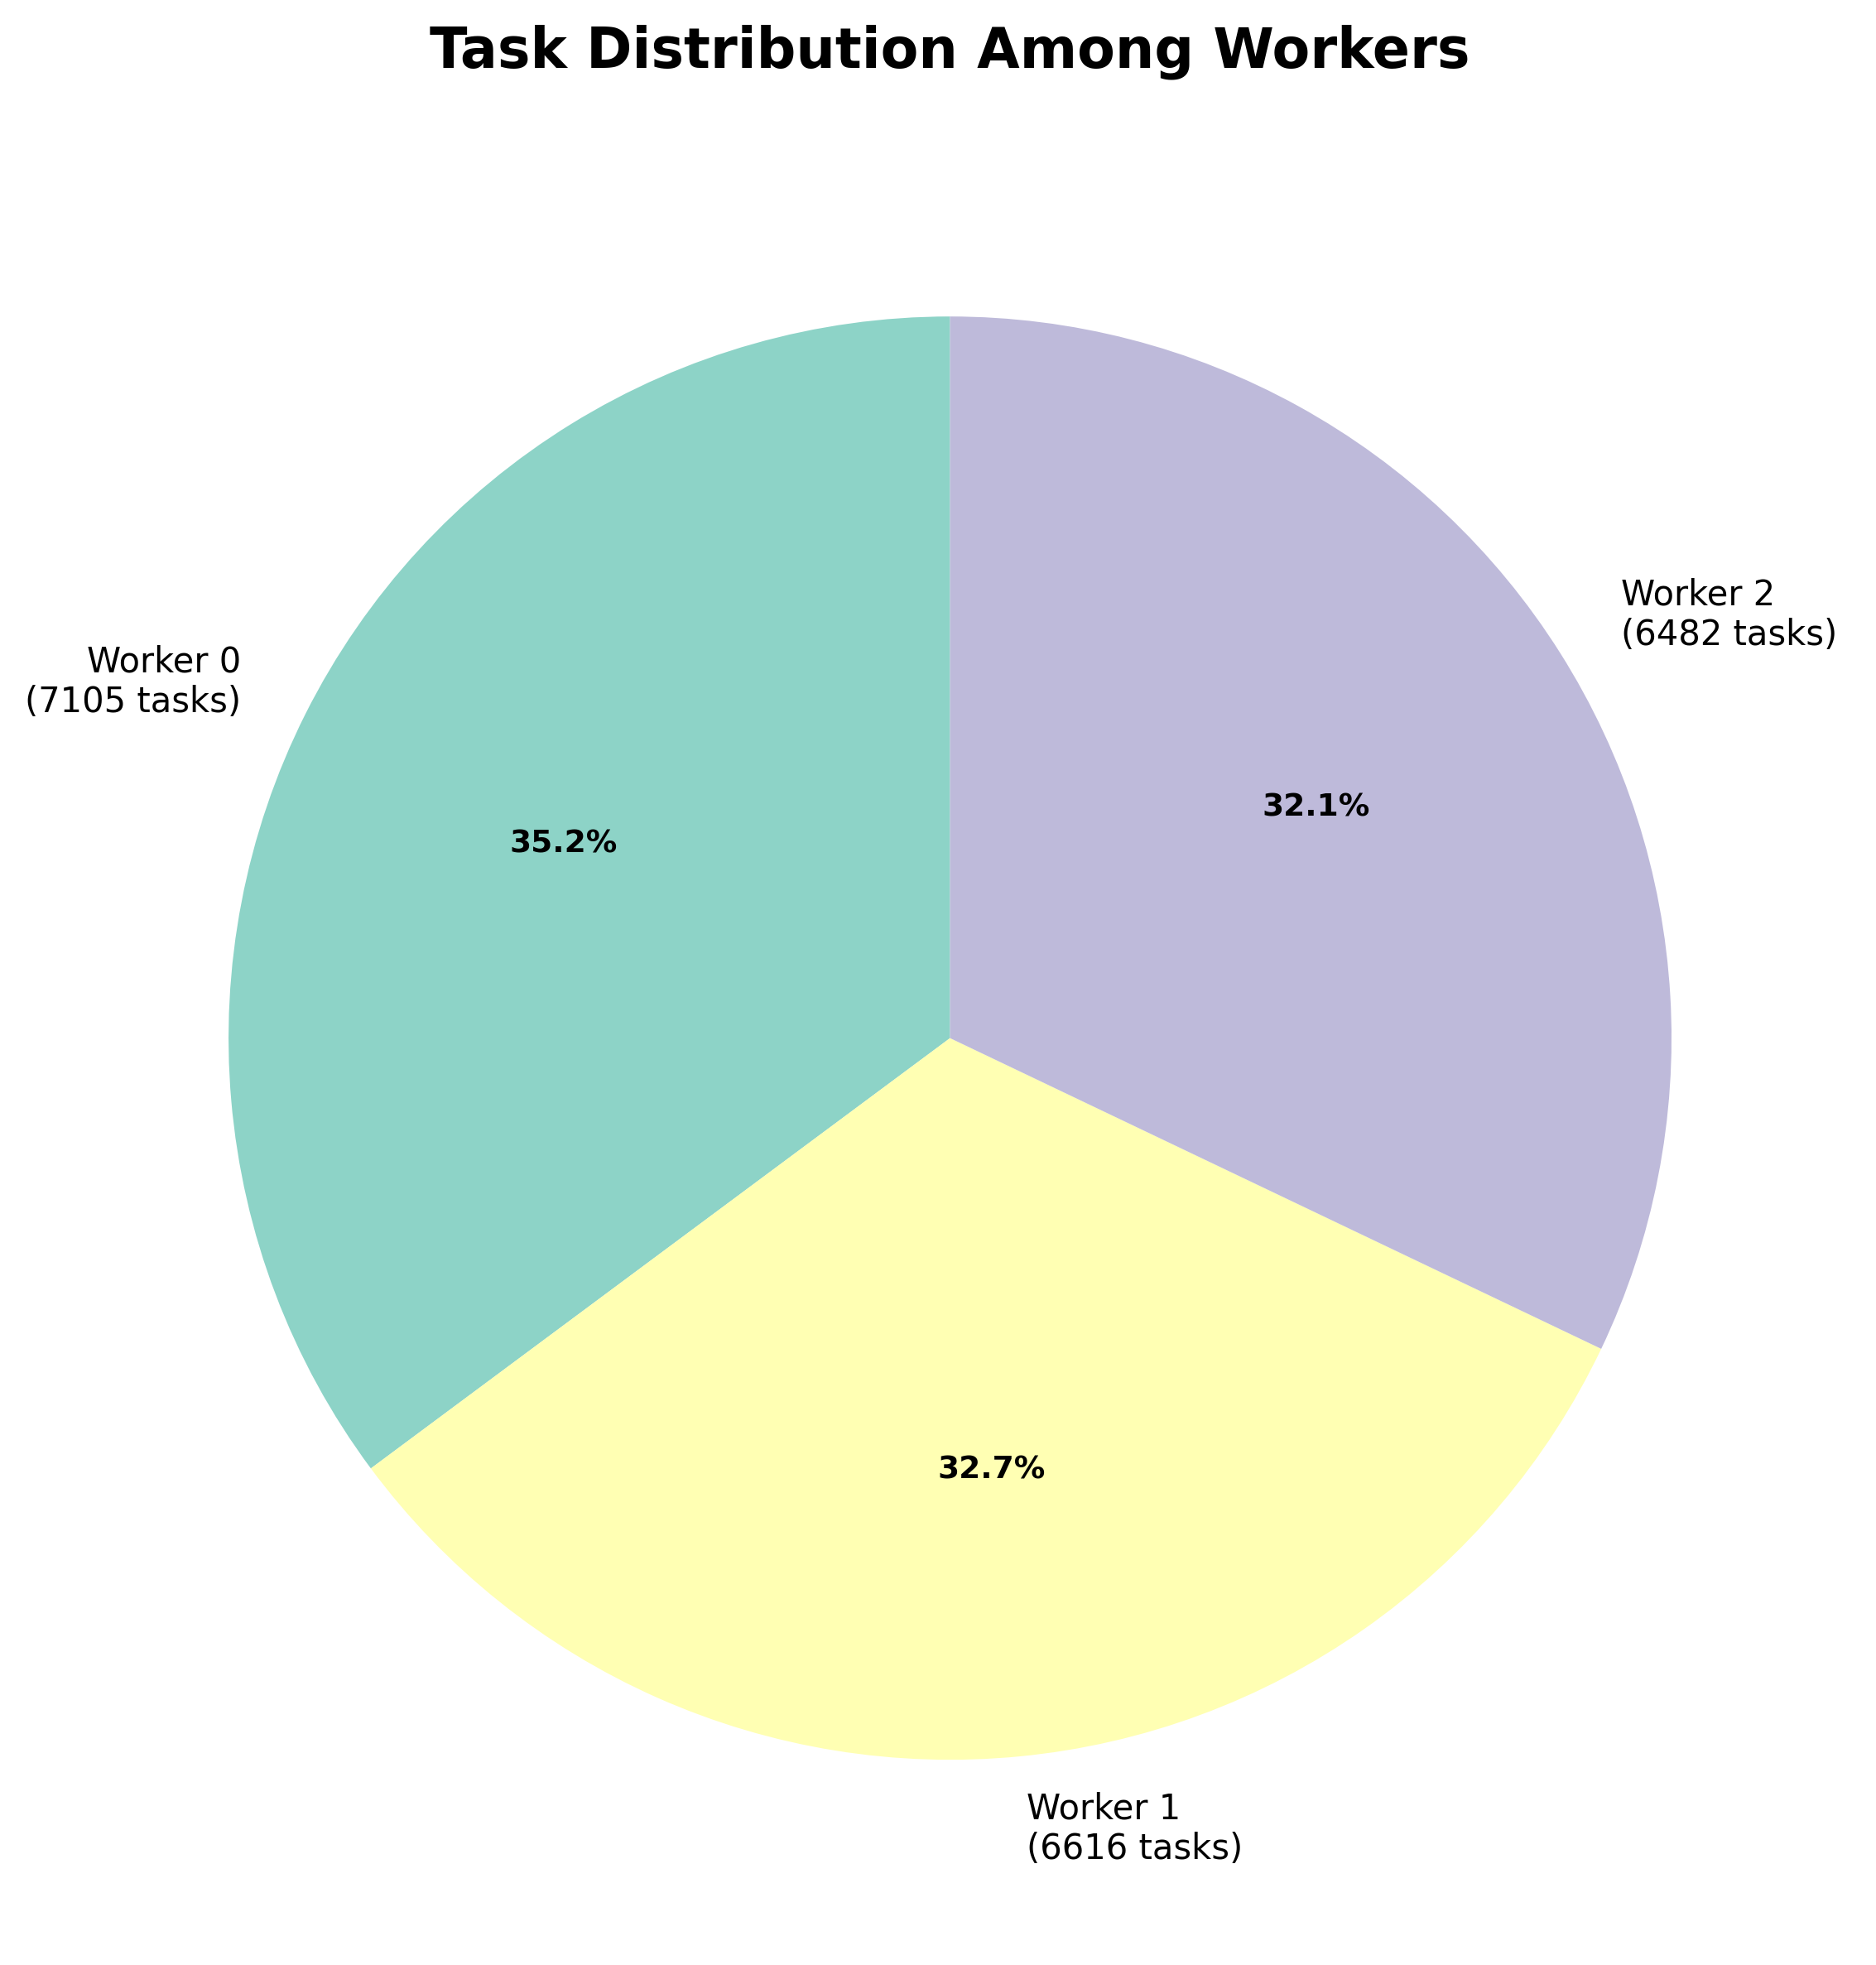
\includegraphics[width=0.5\textwidth]{img/results/variable_computational_demand_sim/active_inference_relative_control_task_distribution_pie.png}
    \caption{AIF – Task Distribution (Demand)}
\end{figure}
\begin{figure}[h]
    \centering
    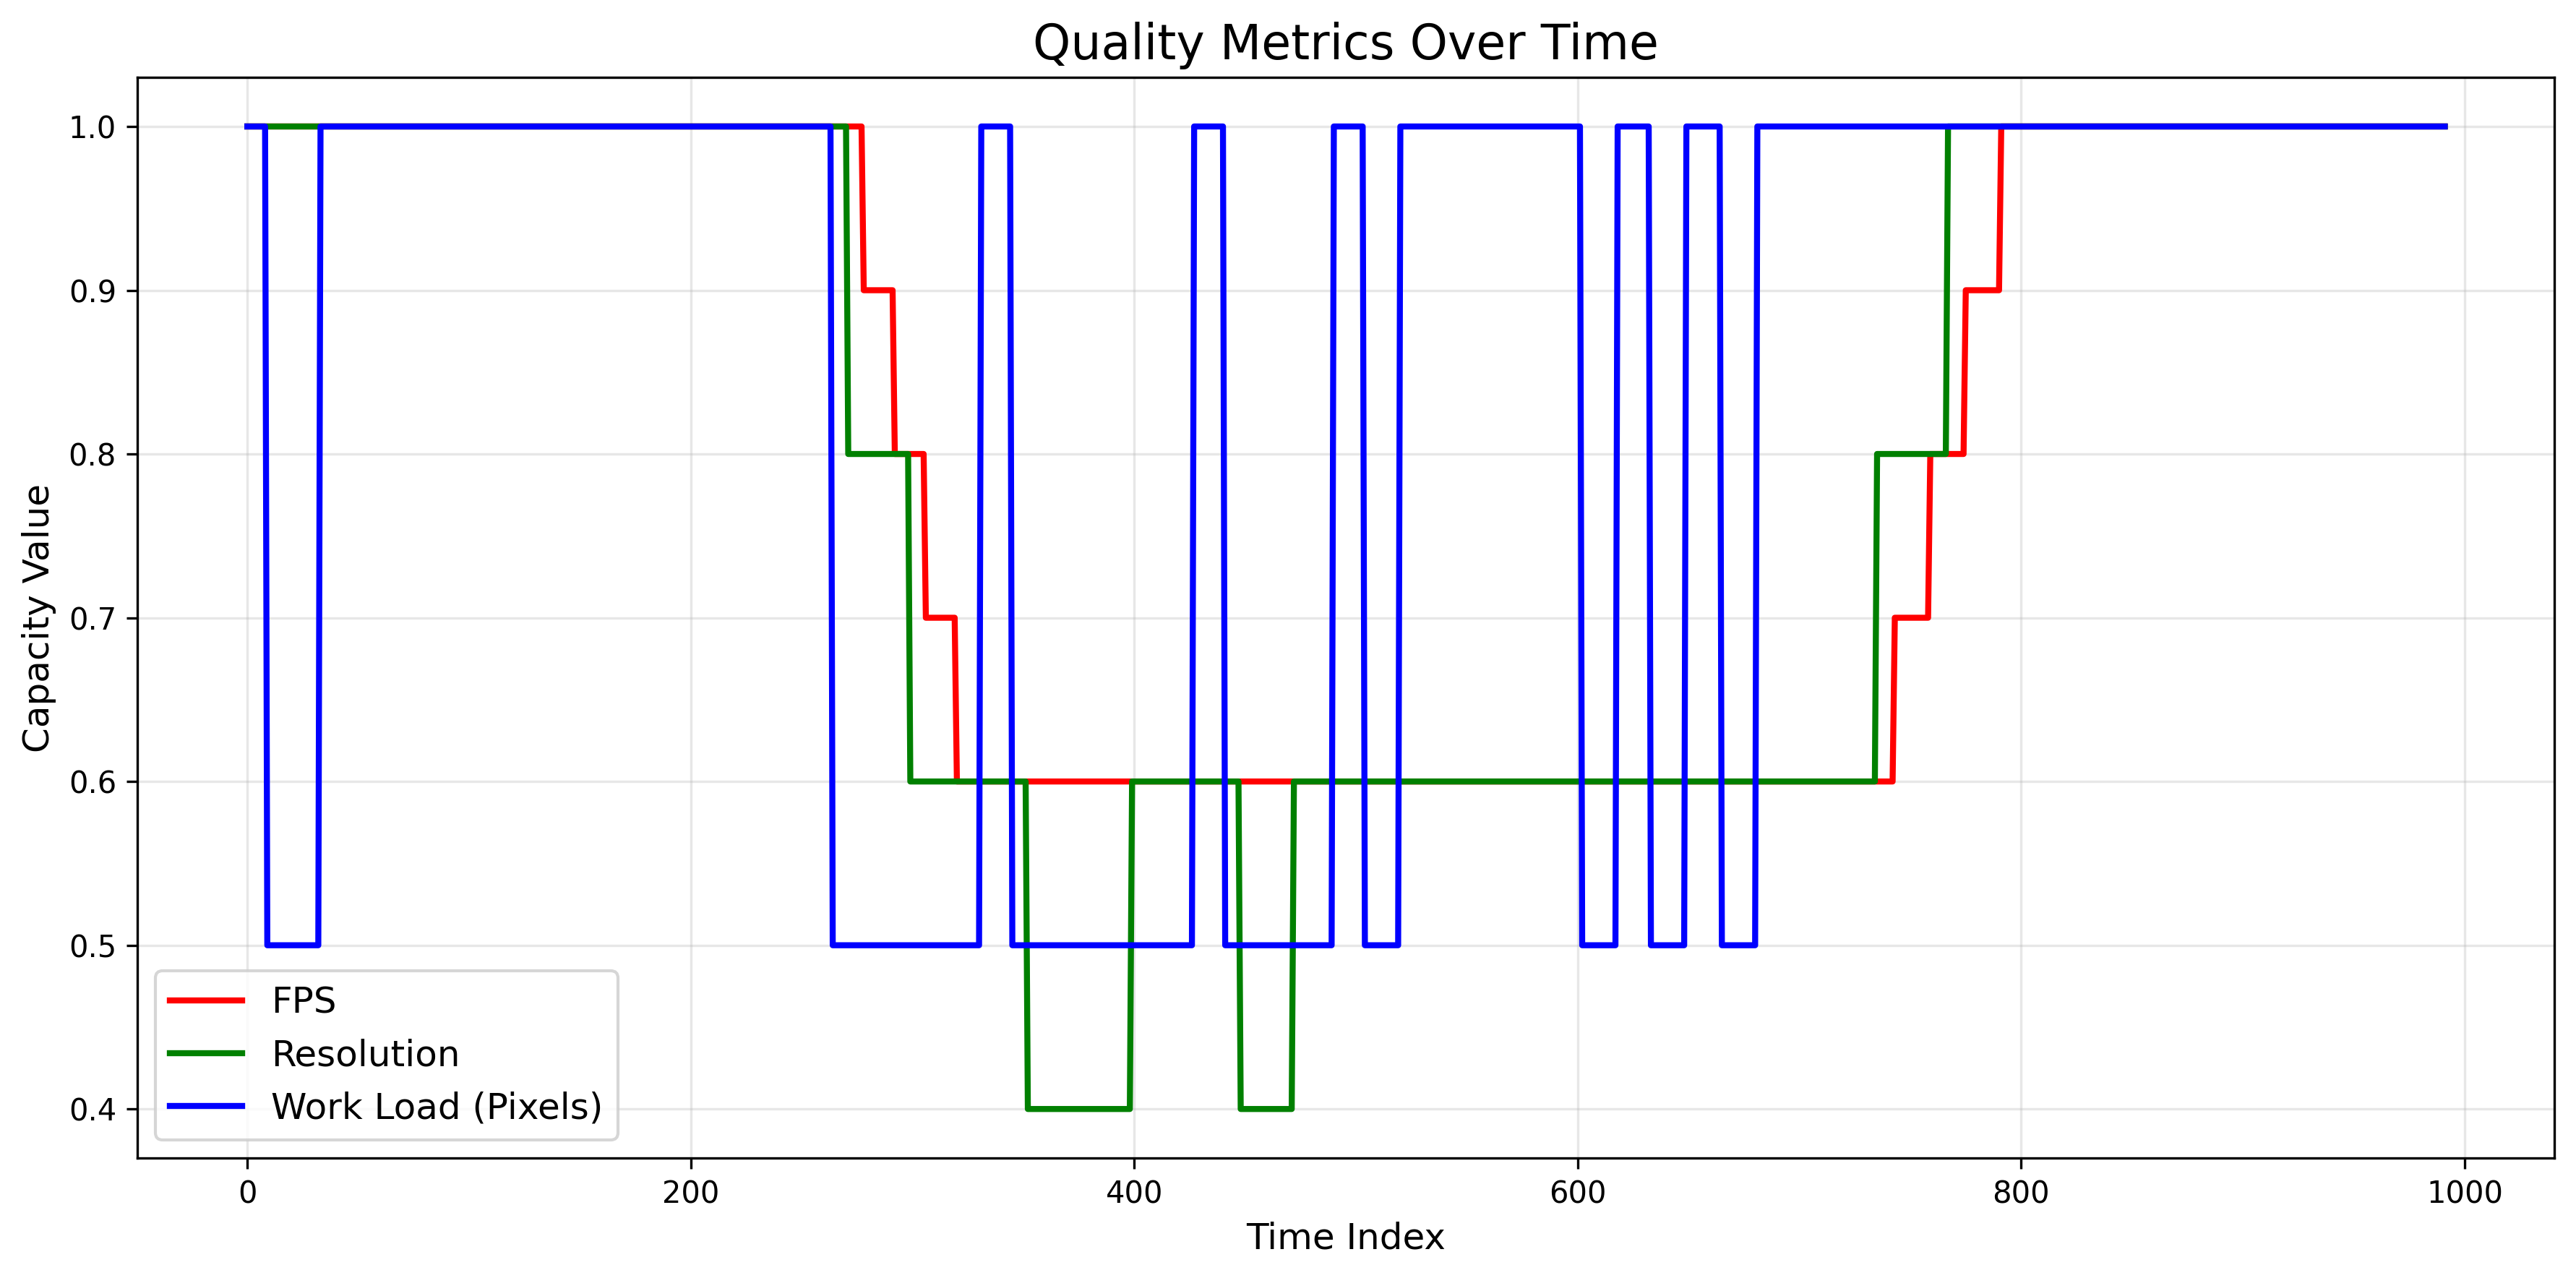
\includegraphics[width=\textwidth]{img/results/variable_computational_demand_sim/heuristic_quality_metrics.png}
    \caption{Heuristic – Quality Metrics Over Time (Demand)}
\end{figure}
\begin{figure}[h]
    \centering
    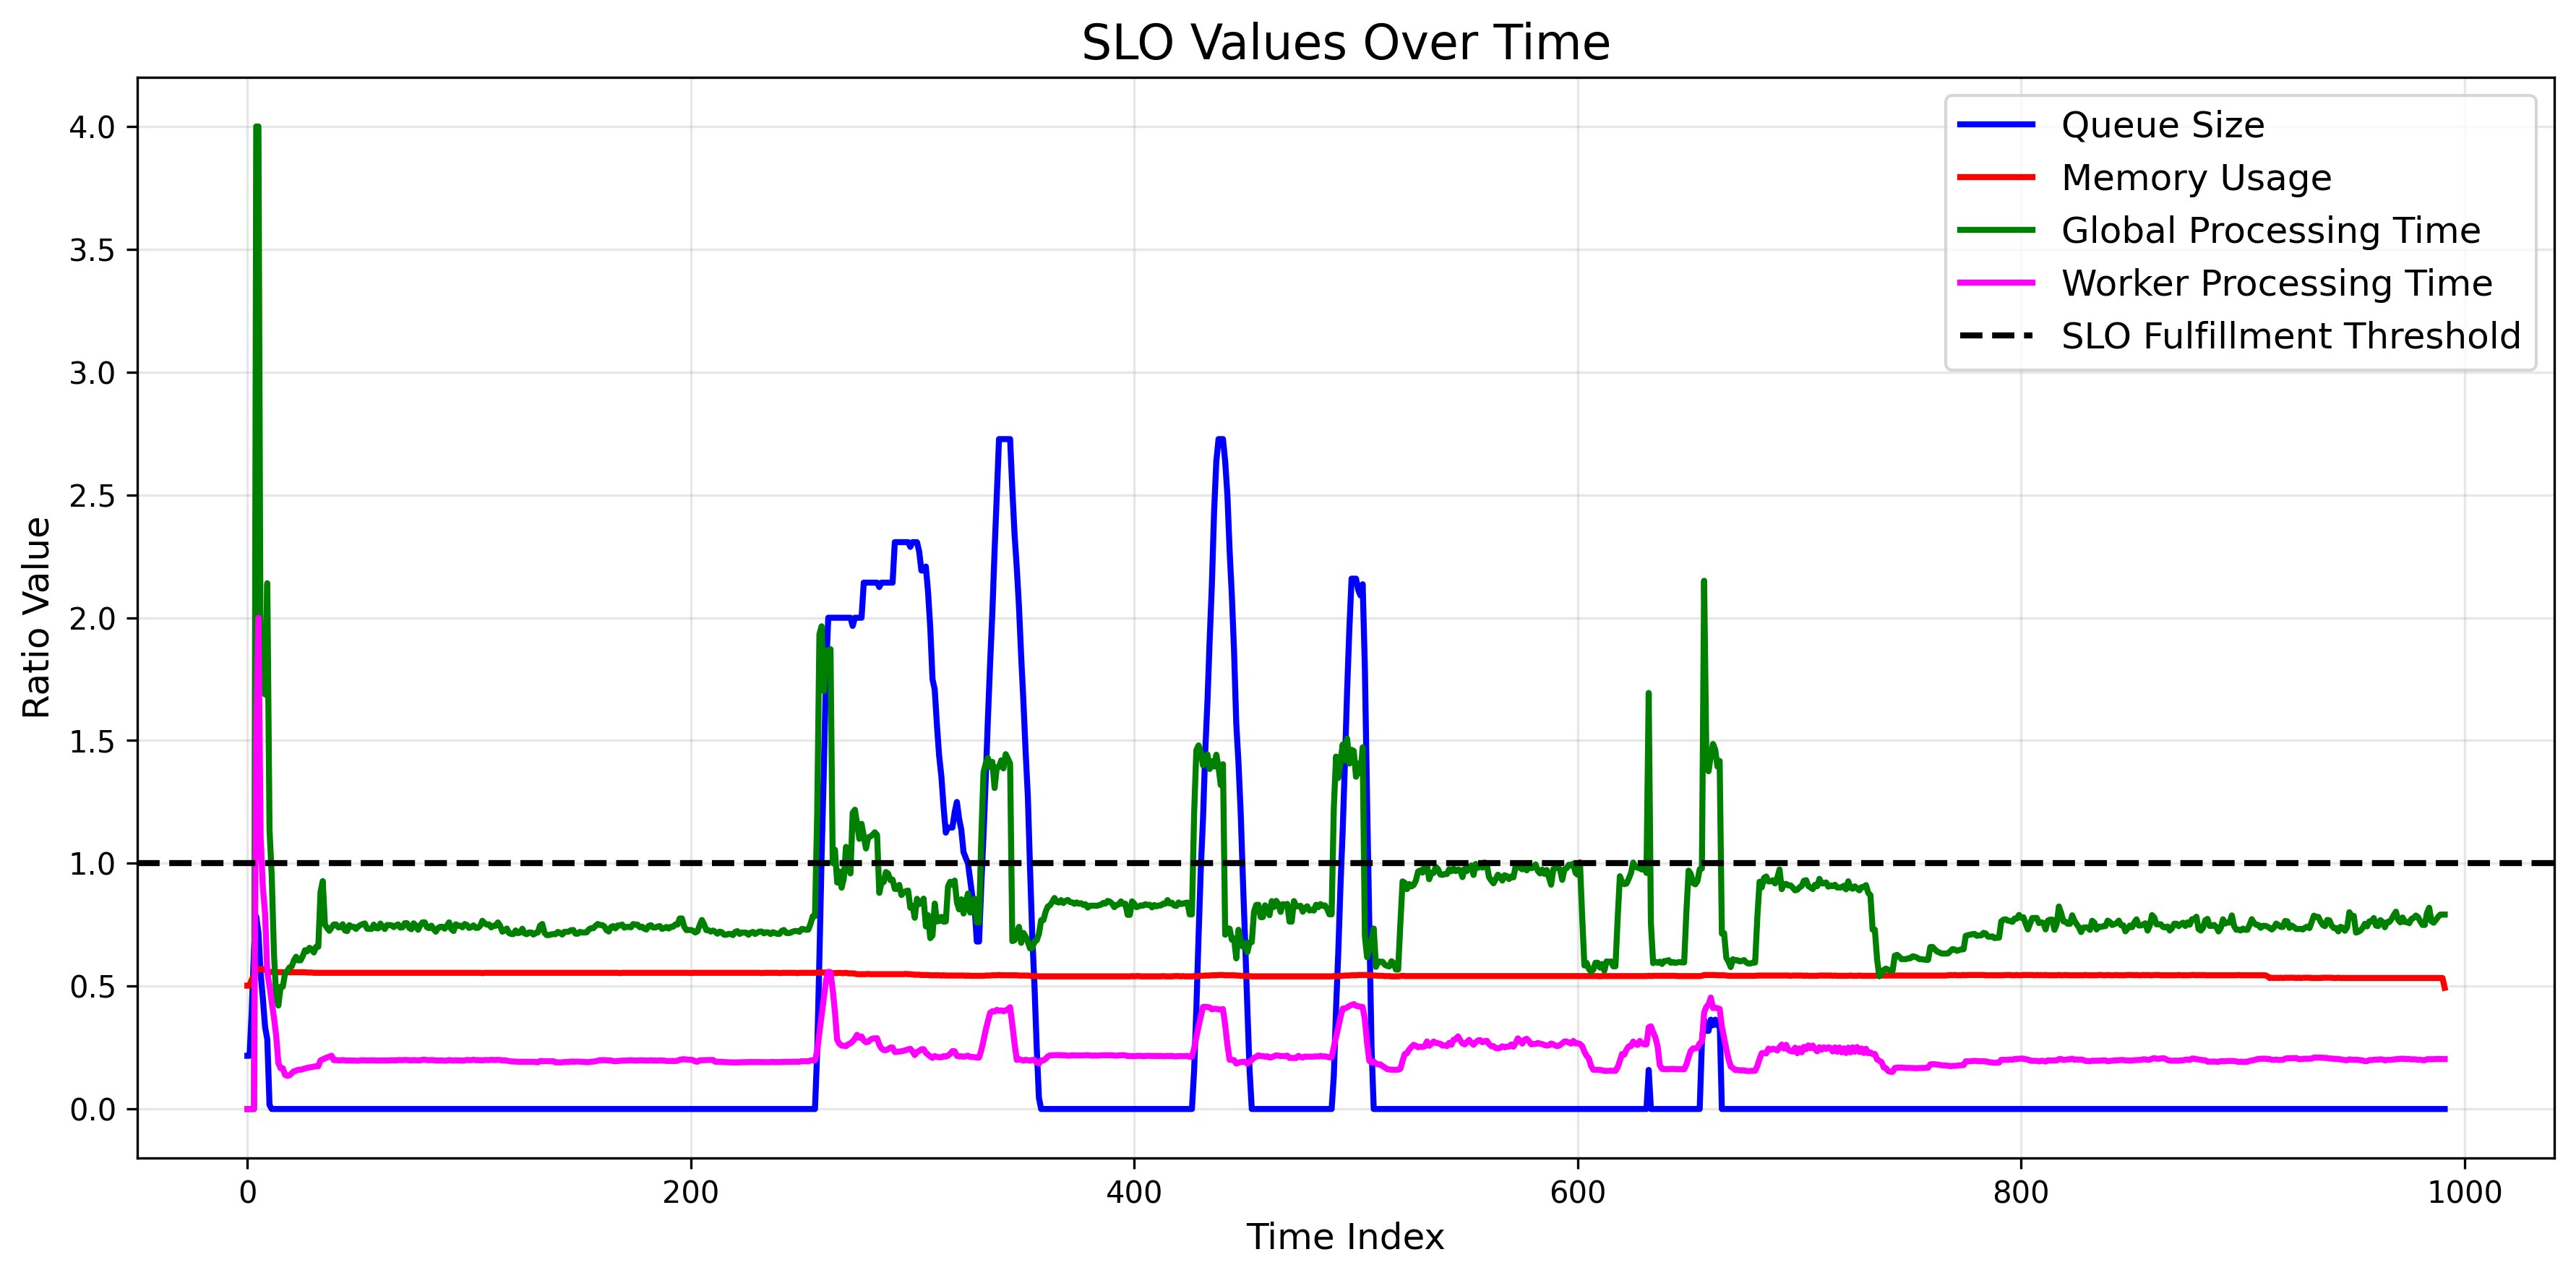
\includegraphics[width=\textwidth]{img/results/variable_computational_demand_sim/heuristic_slo_values.png}
    \caption{Heuristic – SLO Metrics Over Time (Demand)}
\end{figure}
\begin{figure}[h]
    \centering
    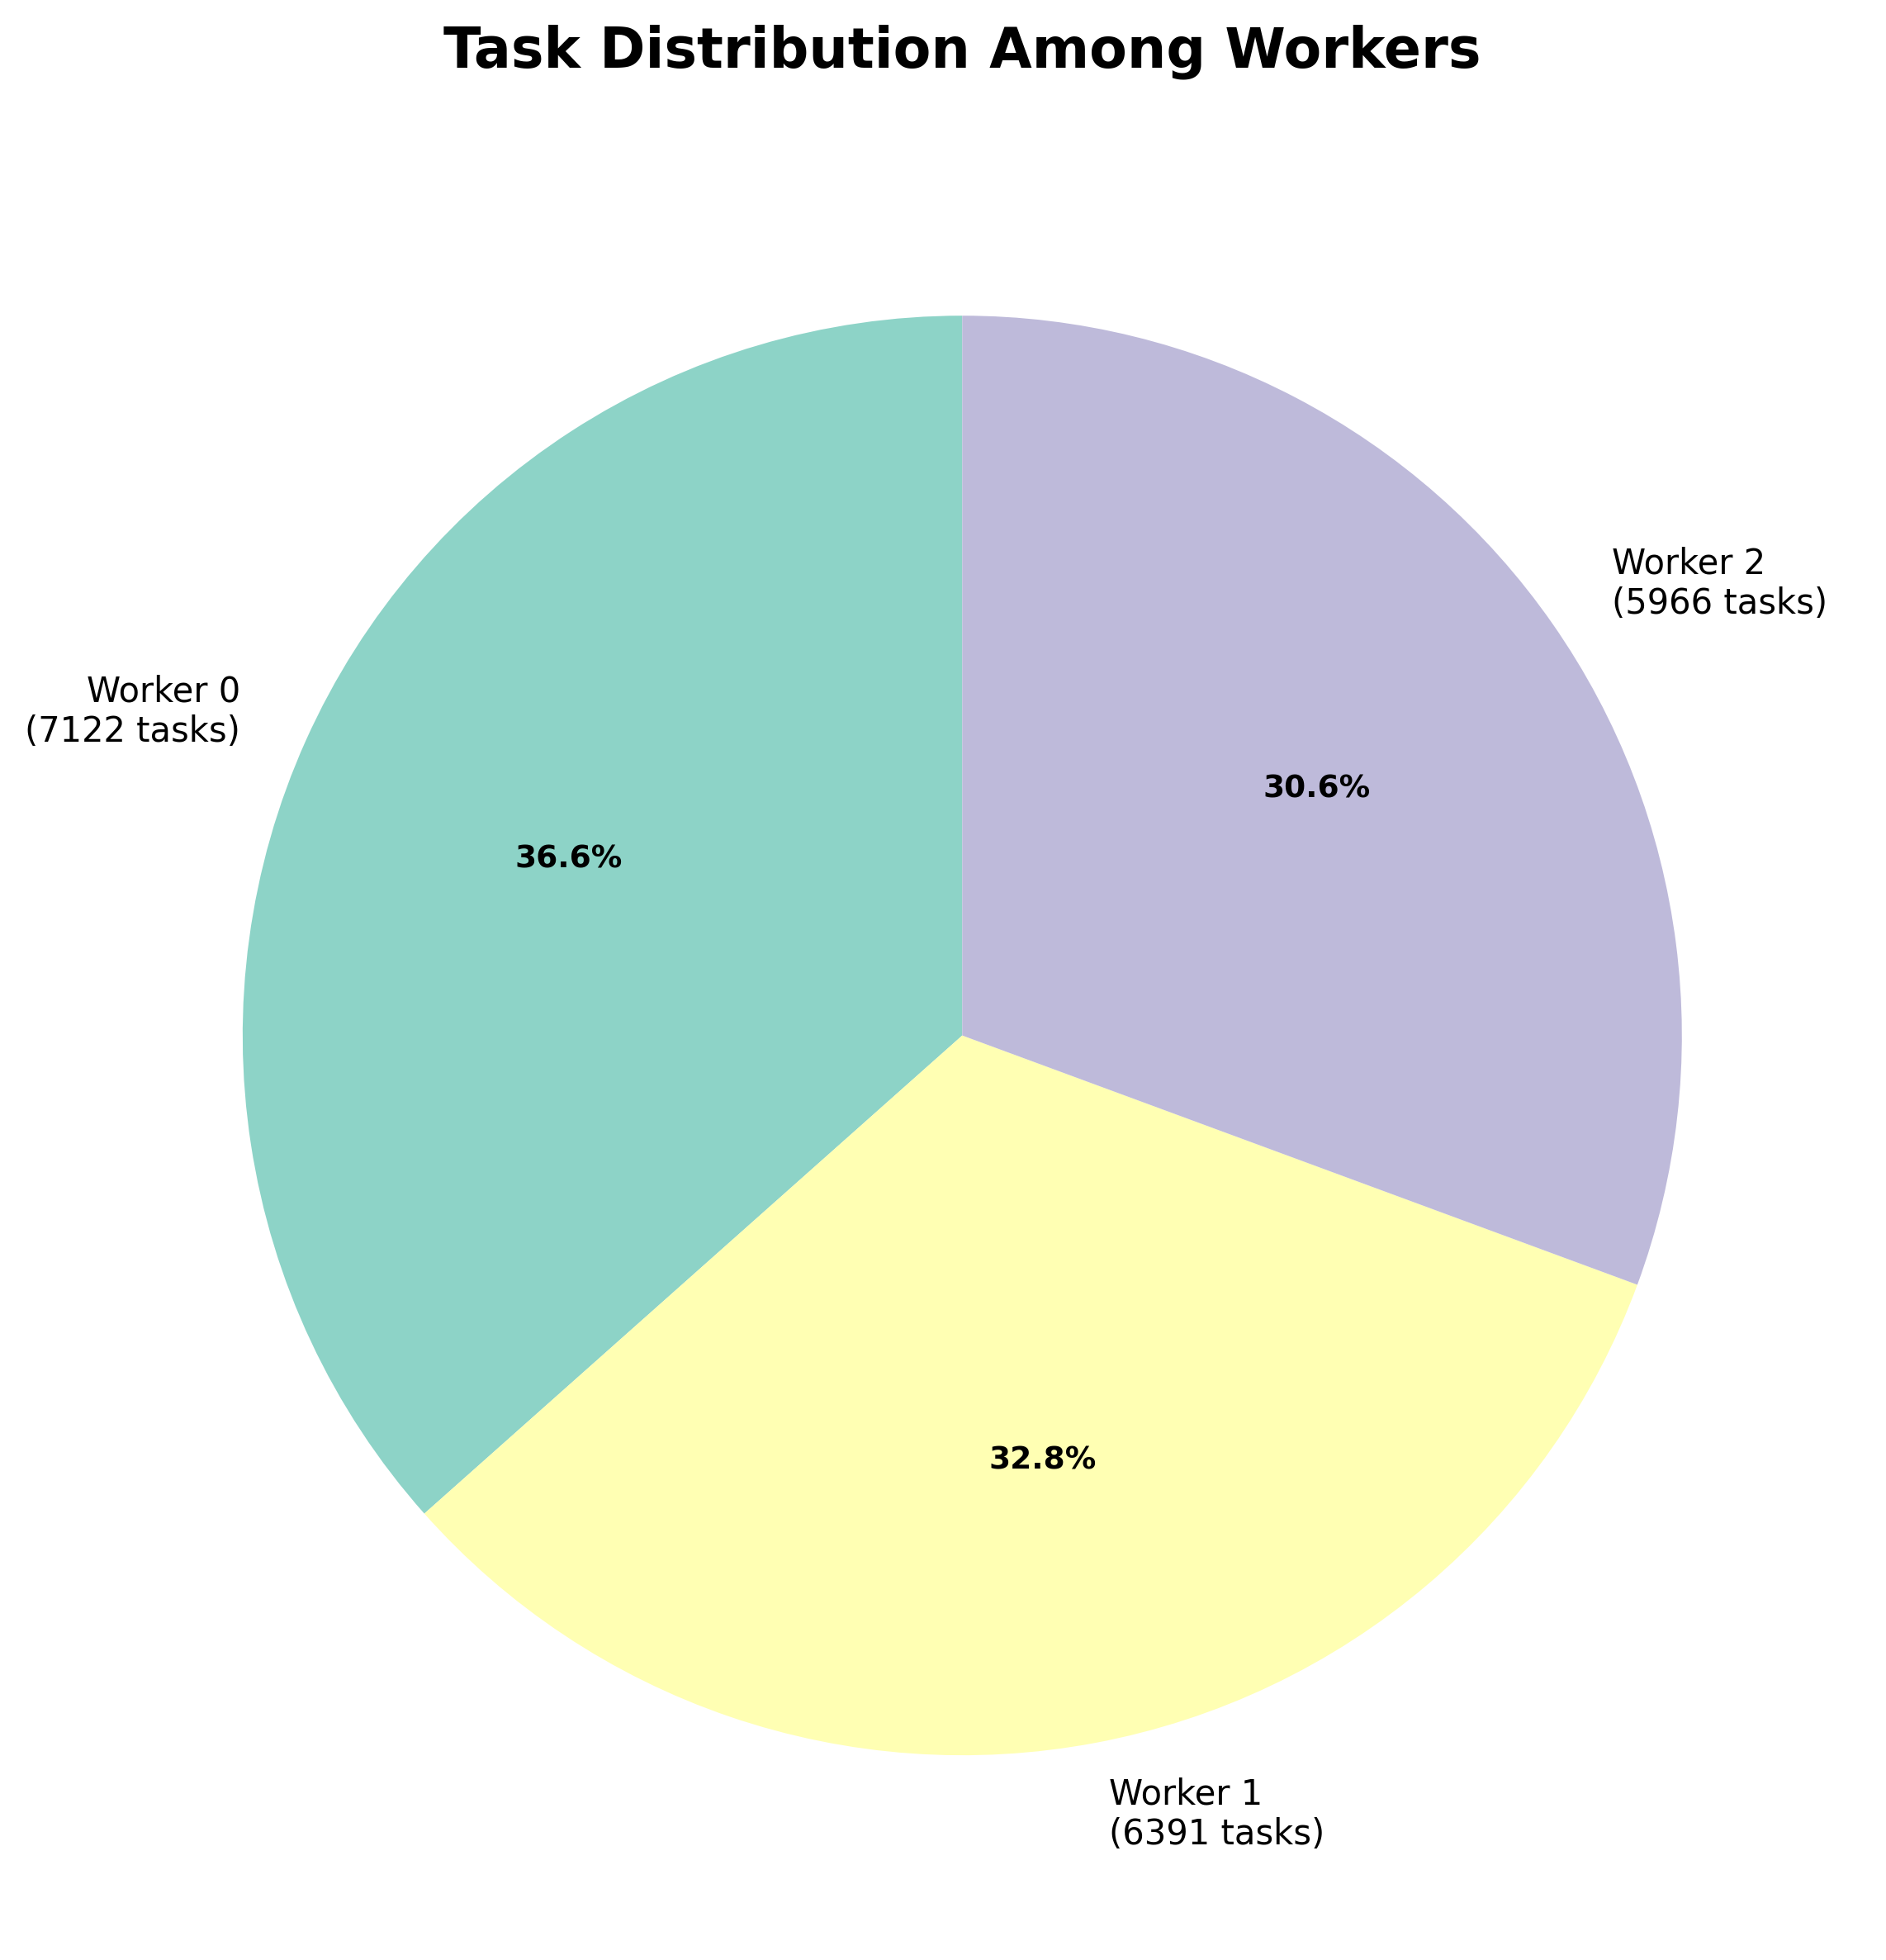
\includegraphics[width=0.5\textwidth]{img/results/variable_computational_demand_sim/heuristic_task_distribution_pie.png}
    \caption{Heuristic – Task Distribution (Demand)}
\end{figure}

\clearpage
\section{Scenario C: Variable Computational Budget}

\subsection*{Active Inference Agent}
\begin{table}[h]
\centering
\caption{Budget – Active Inference}
\label{tab:budget_active_inference}
\begin{tabular}{lr}
\toprule
Metric & Value \\
\midrule
Total Simulation Timesteps & 884 \\
\% Time All SLOs Met & 0.9615 \\
Average SLO Fulfillment Rate & 0.9827 \\
Average Overall Stream Quality Score & 0.6077 \\
Max Consecutive SLO Violations & 31 \\
Time to Reach Stable Configuration & 1.0000 \\
Queue Size SLO Fulfillment Rate & 0.9717 \\
Memory Usage SLO Fulfillment Rate & 1.0000 \\
Global Processing Time SLO Fulfillment Rate & 0.9638 \\
Worker Processing Time SLO Fulfillment Rate & 0.9955 \\
Queue Size Violation Severity (Avg) & 0.3963 \\
Worker Proc. Time Violation Severity (Avg) & 2.1070 \\
\bottomrule
\end{tabular}
\end{table}


\subsection*{Heuristic Agent}
\begin{table}[h]
\centering
\caption{Budget – Heuristic}
\label{tab:budget_heuristic}
\begin{tabular}{lr}
\toprule
Metric & Value \\
\midrule
Total Simulation Timesteps & 916 \\
\% Time All SLOs Met & 0.8843 \\
Average SLO Fulfillment Rate & 0.9675 \\
Average Overall Stream Quality Score & 0.7541 \\
Max Consecutive SLO Violations & 18 \\
Time to Reach Stable Configuration & 0.9412 \\
Queue Size SLO Fulfillment Rate & 0.9891 \\
Memory Usage SLO Fulfillment Rate & 1.0000 \\
Global Processing Time SLO Fulfillment Rate & 0.8854 \\
Worker Processing Time SLO Fulfillment Rate & 0.9956 \\
Queue Size Violation Severity (Avg) & 0.2418 \\
Worker Proc. Time Violation Severity (Avg) & 1.0020 \\
\bottomrule
\end{tabular}
\end{table}


\subsection*{Plots}
\begin{figure}[h]
    \centering
    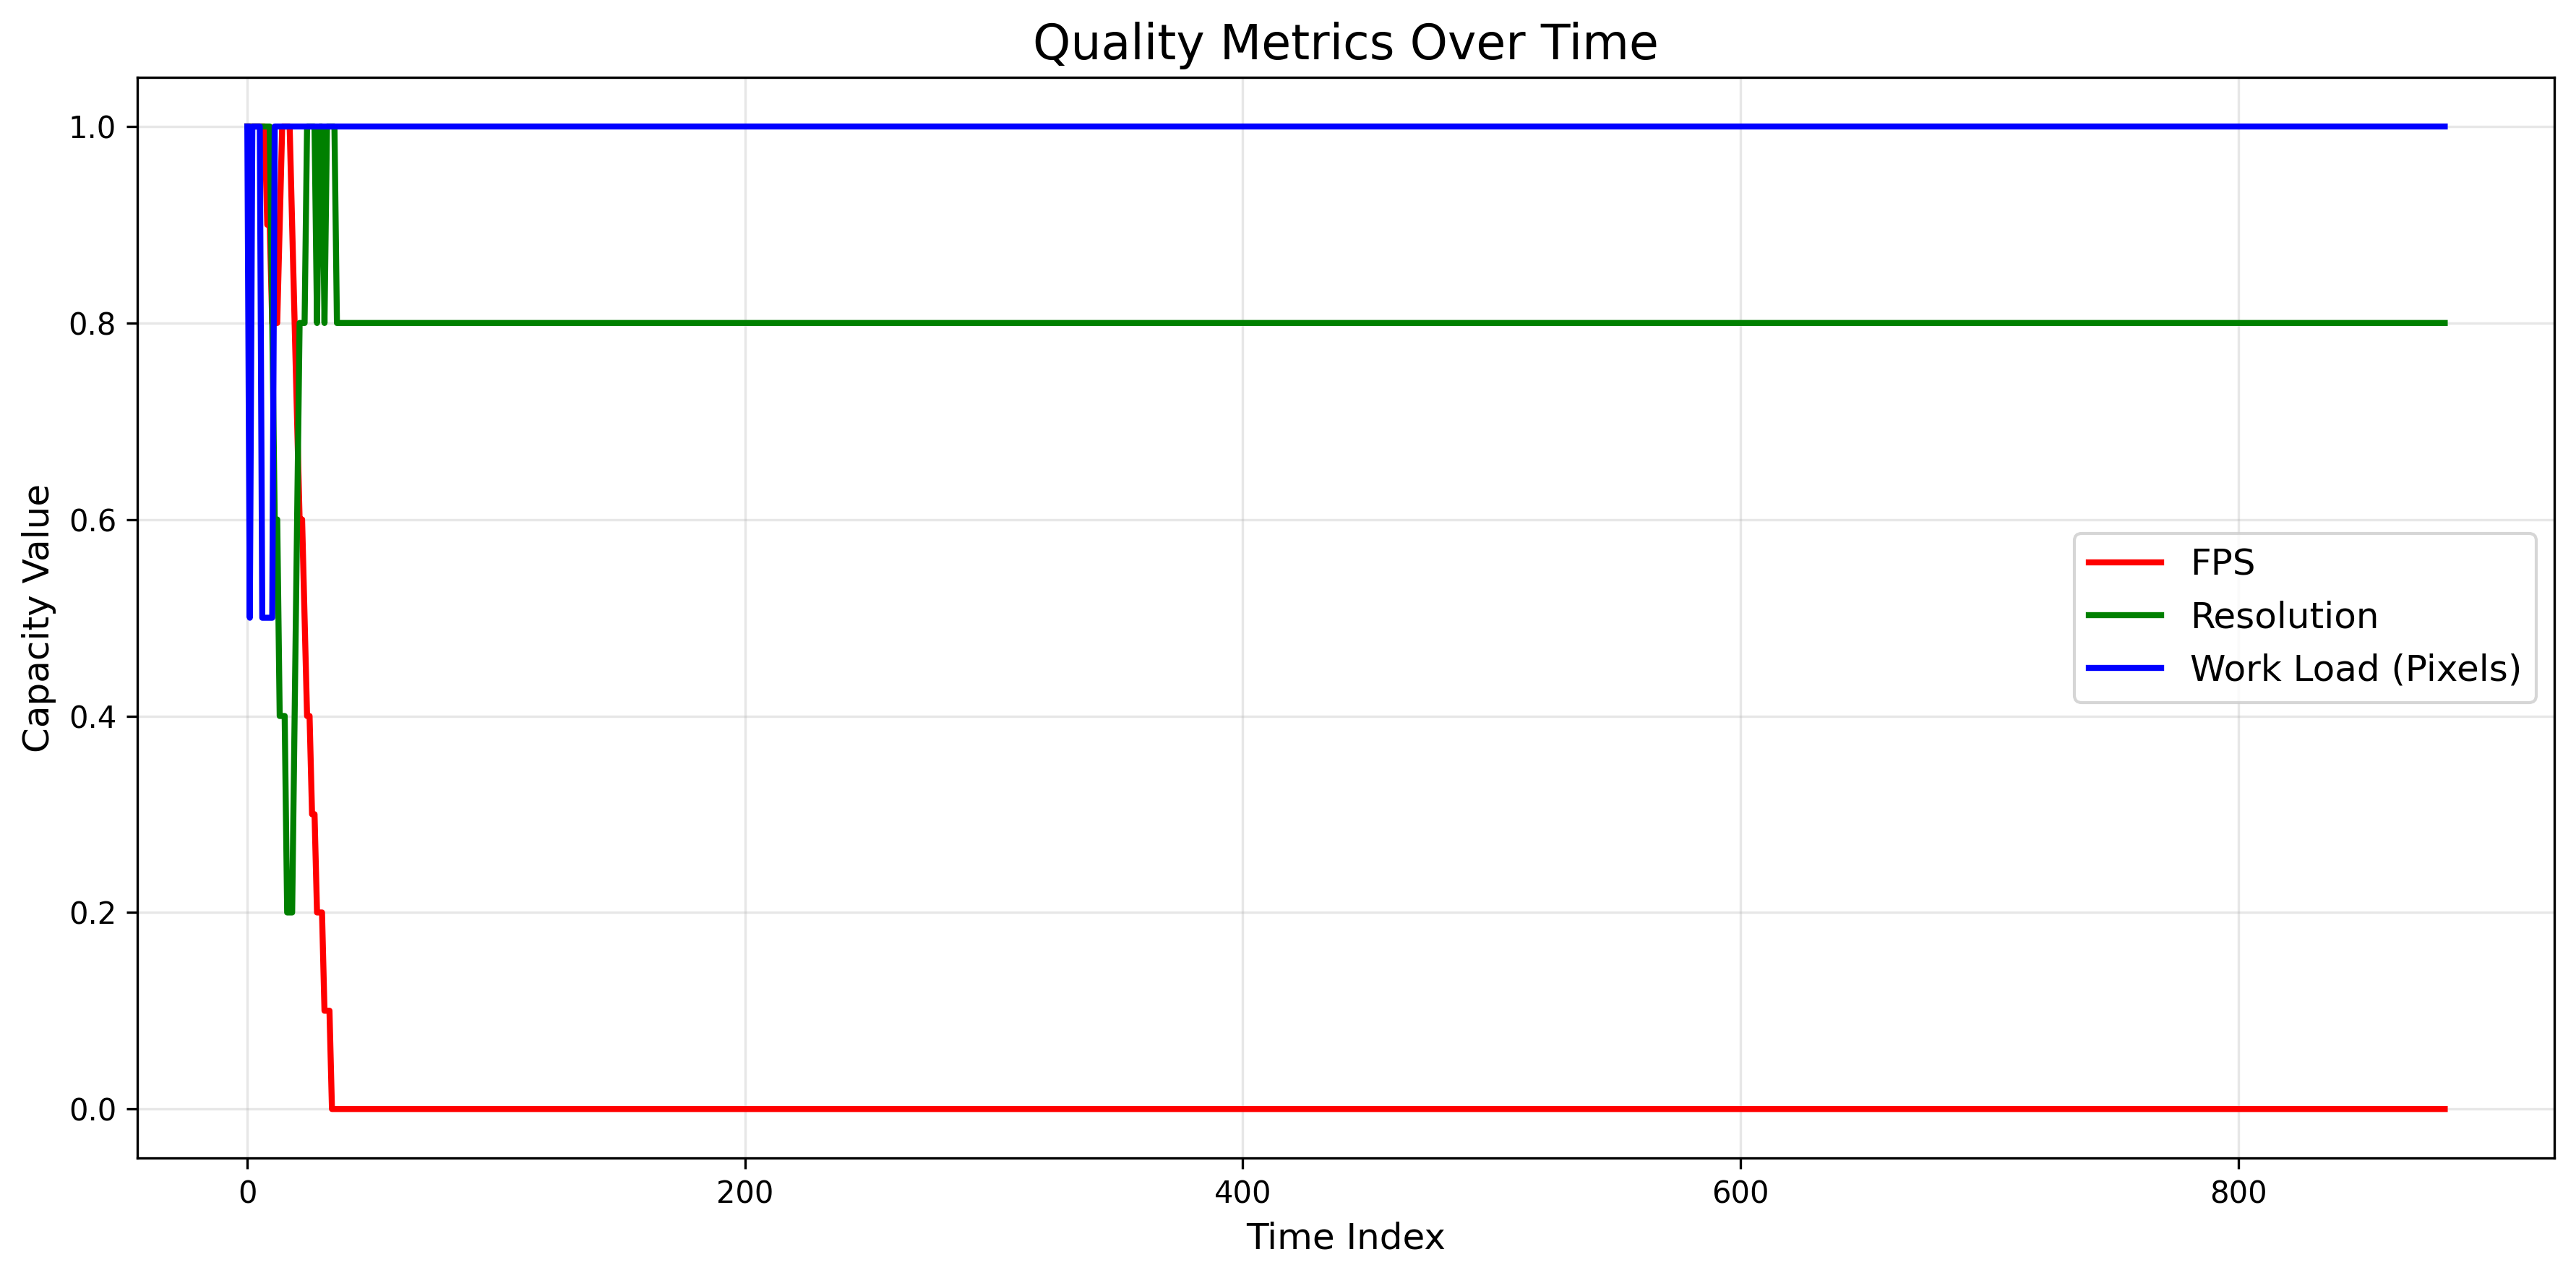
\includegraphics[width=\textwidth]{img/results/variable_computational_budget_sim/active_inference_relative_control_quality_metrics.png}
    \caption{AIF – Quality Metrics Over Time (Budget)}
\end{figure}
\begin{figure}[h]
    \centering
    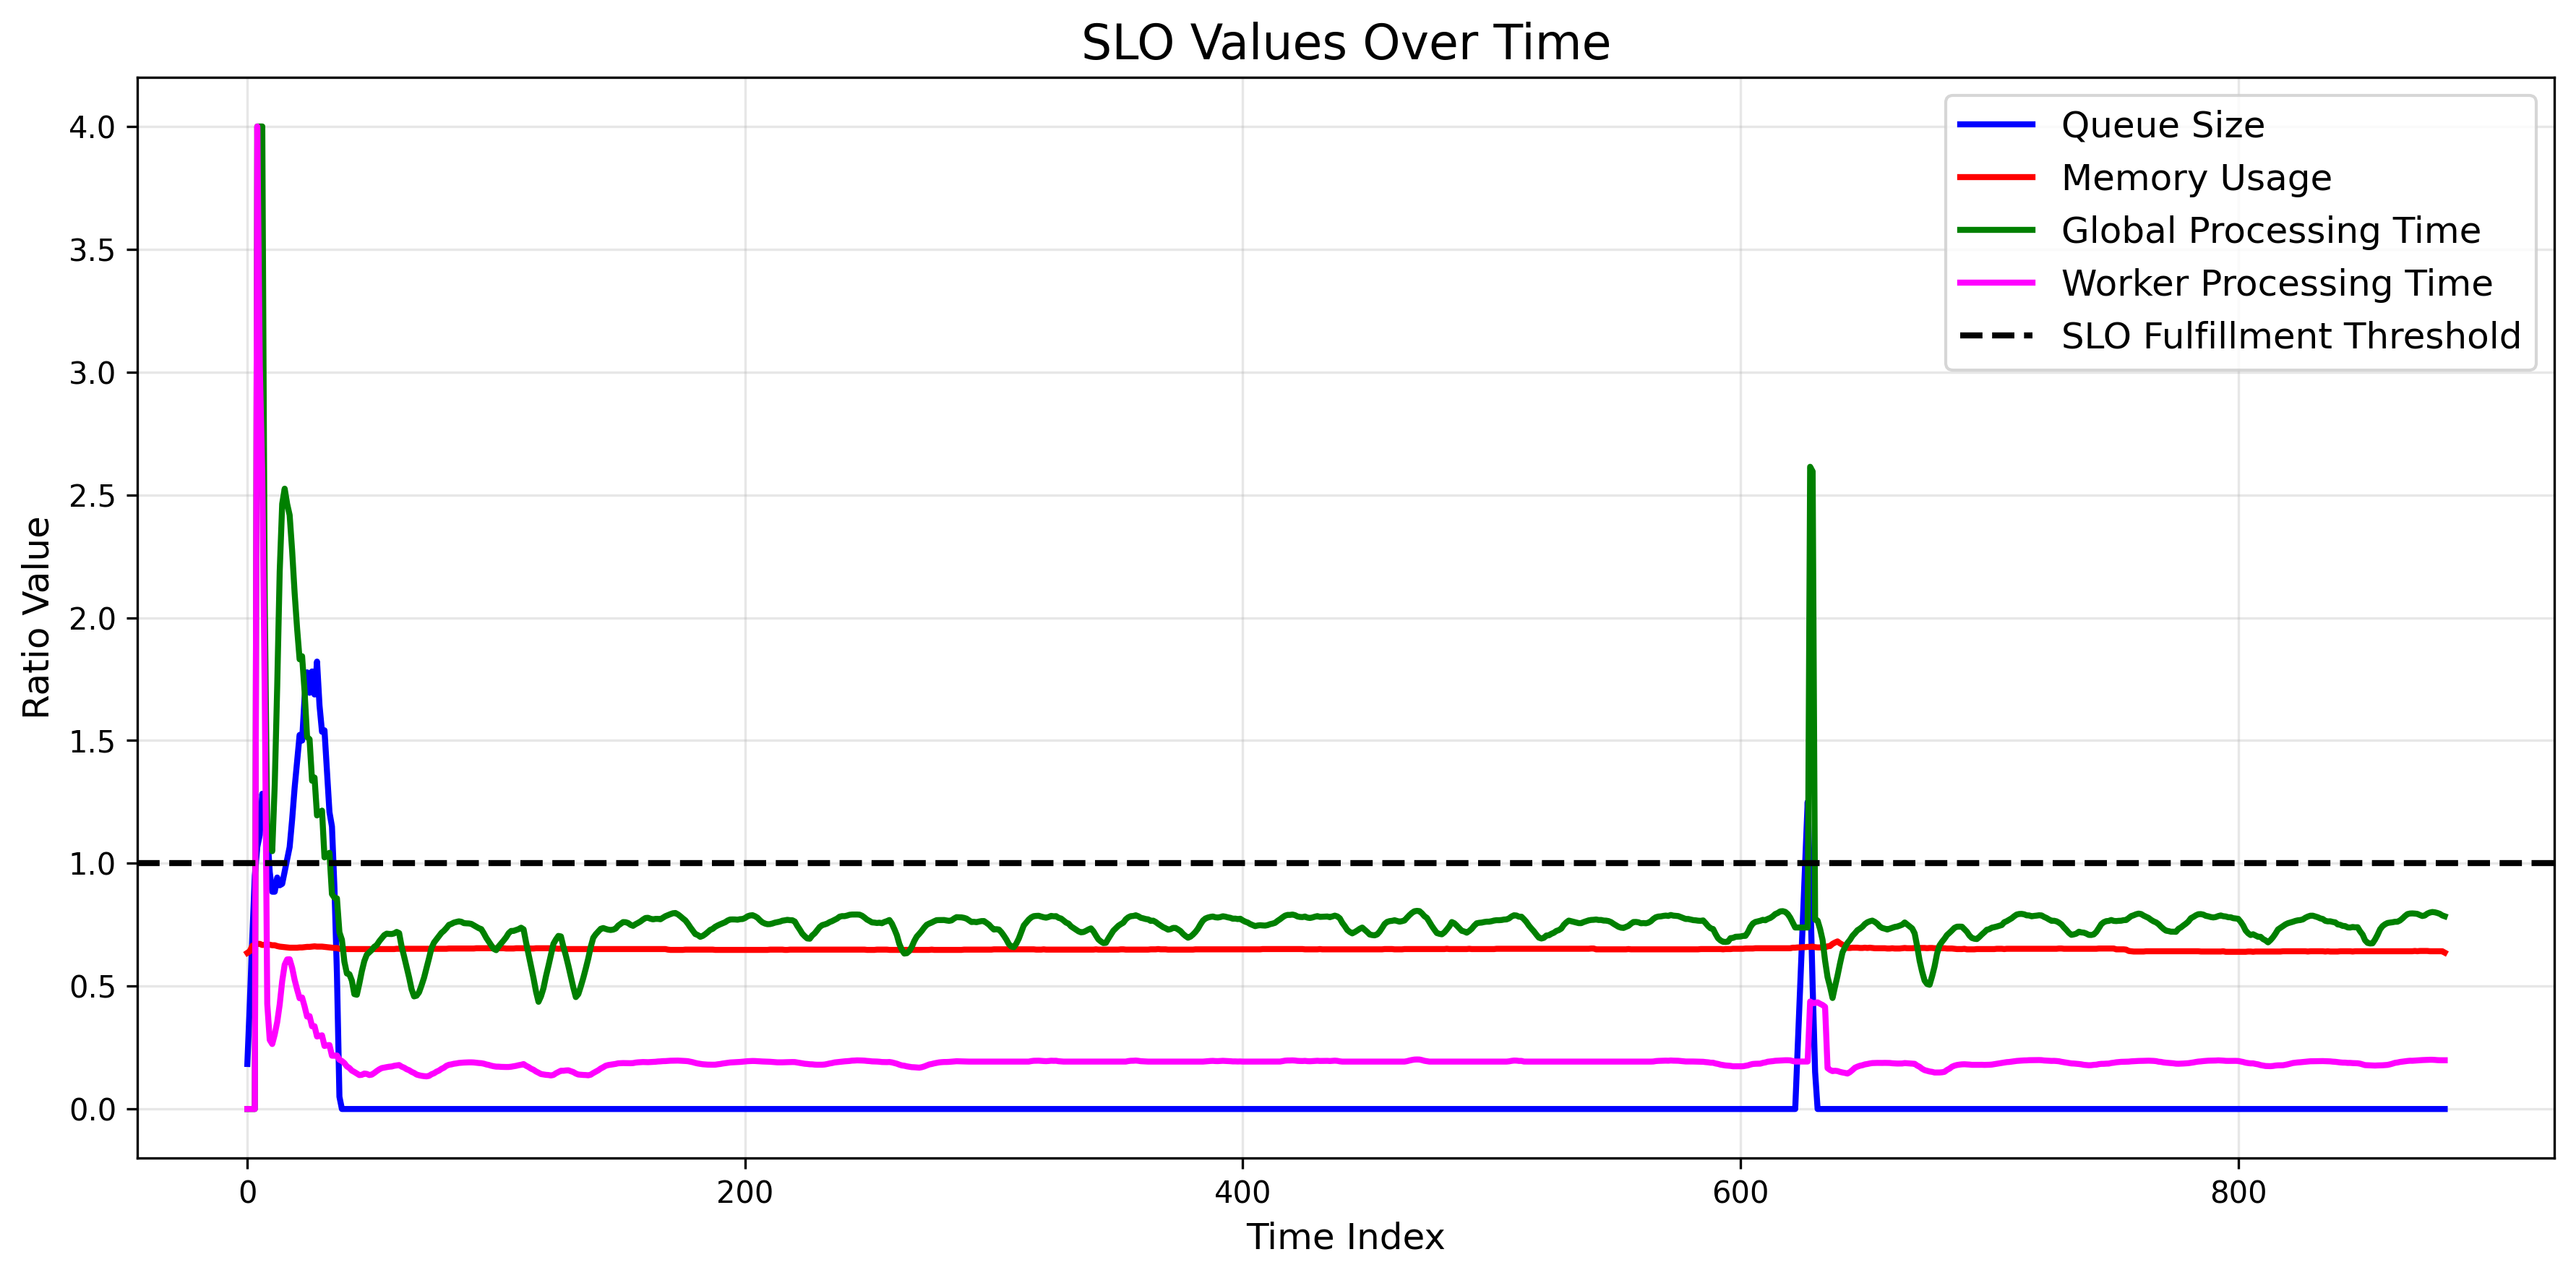
\includegraphics[width=\textwidth]{img/results/variable_computational_budget_sim/active_inference_relative_control_slo_values.png}
    \caption{AIF – SLO Metrics Over Time (Budget)}
\end{figure}
\begin{figure}[h]
    \centering
    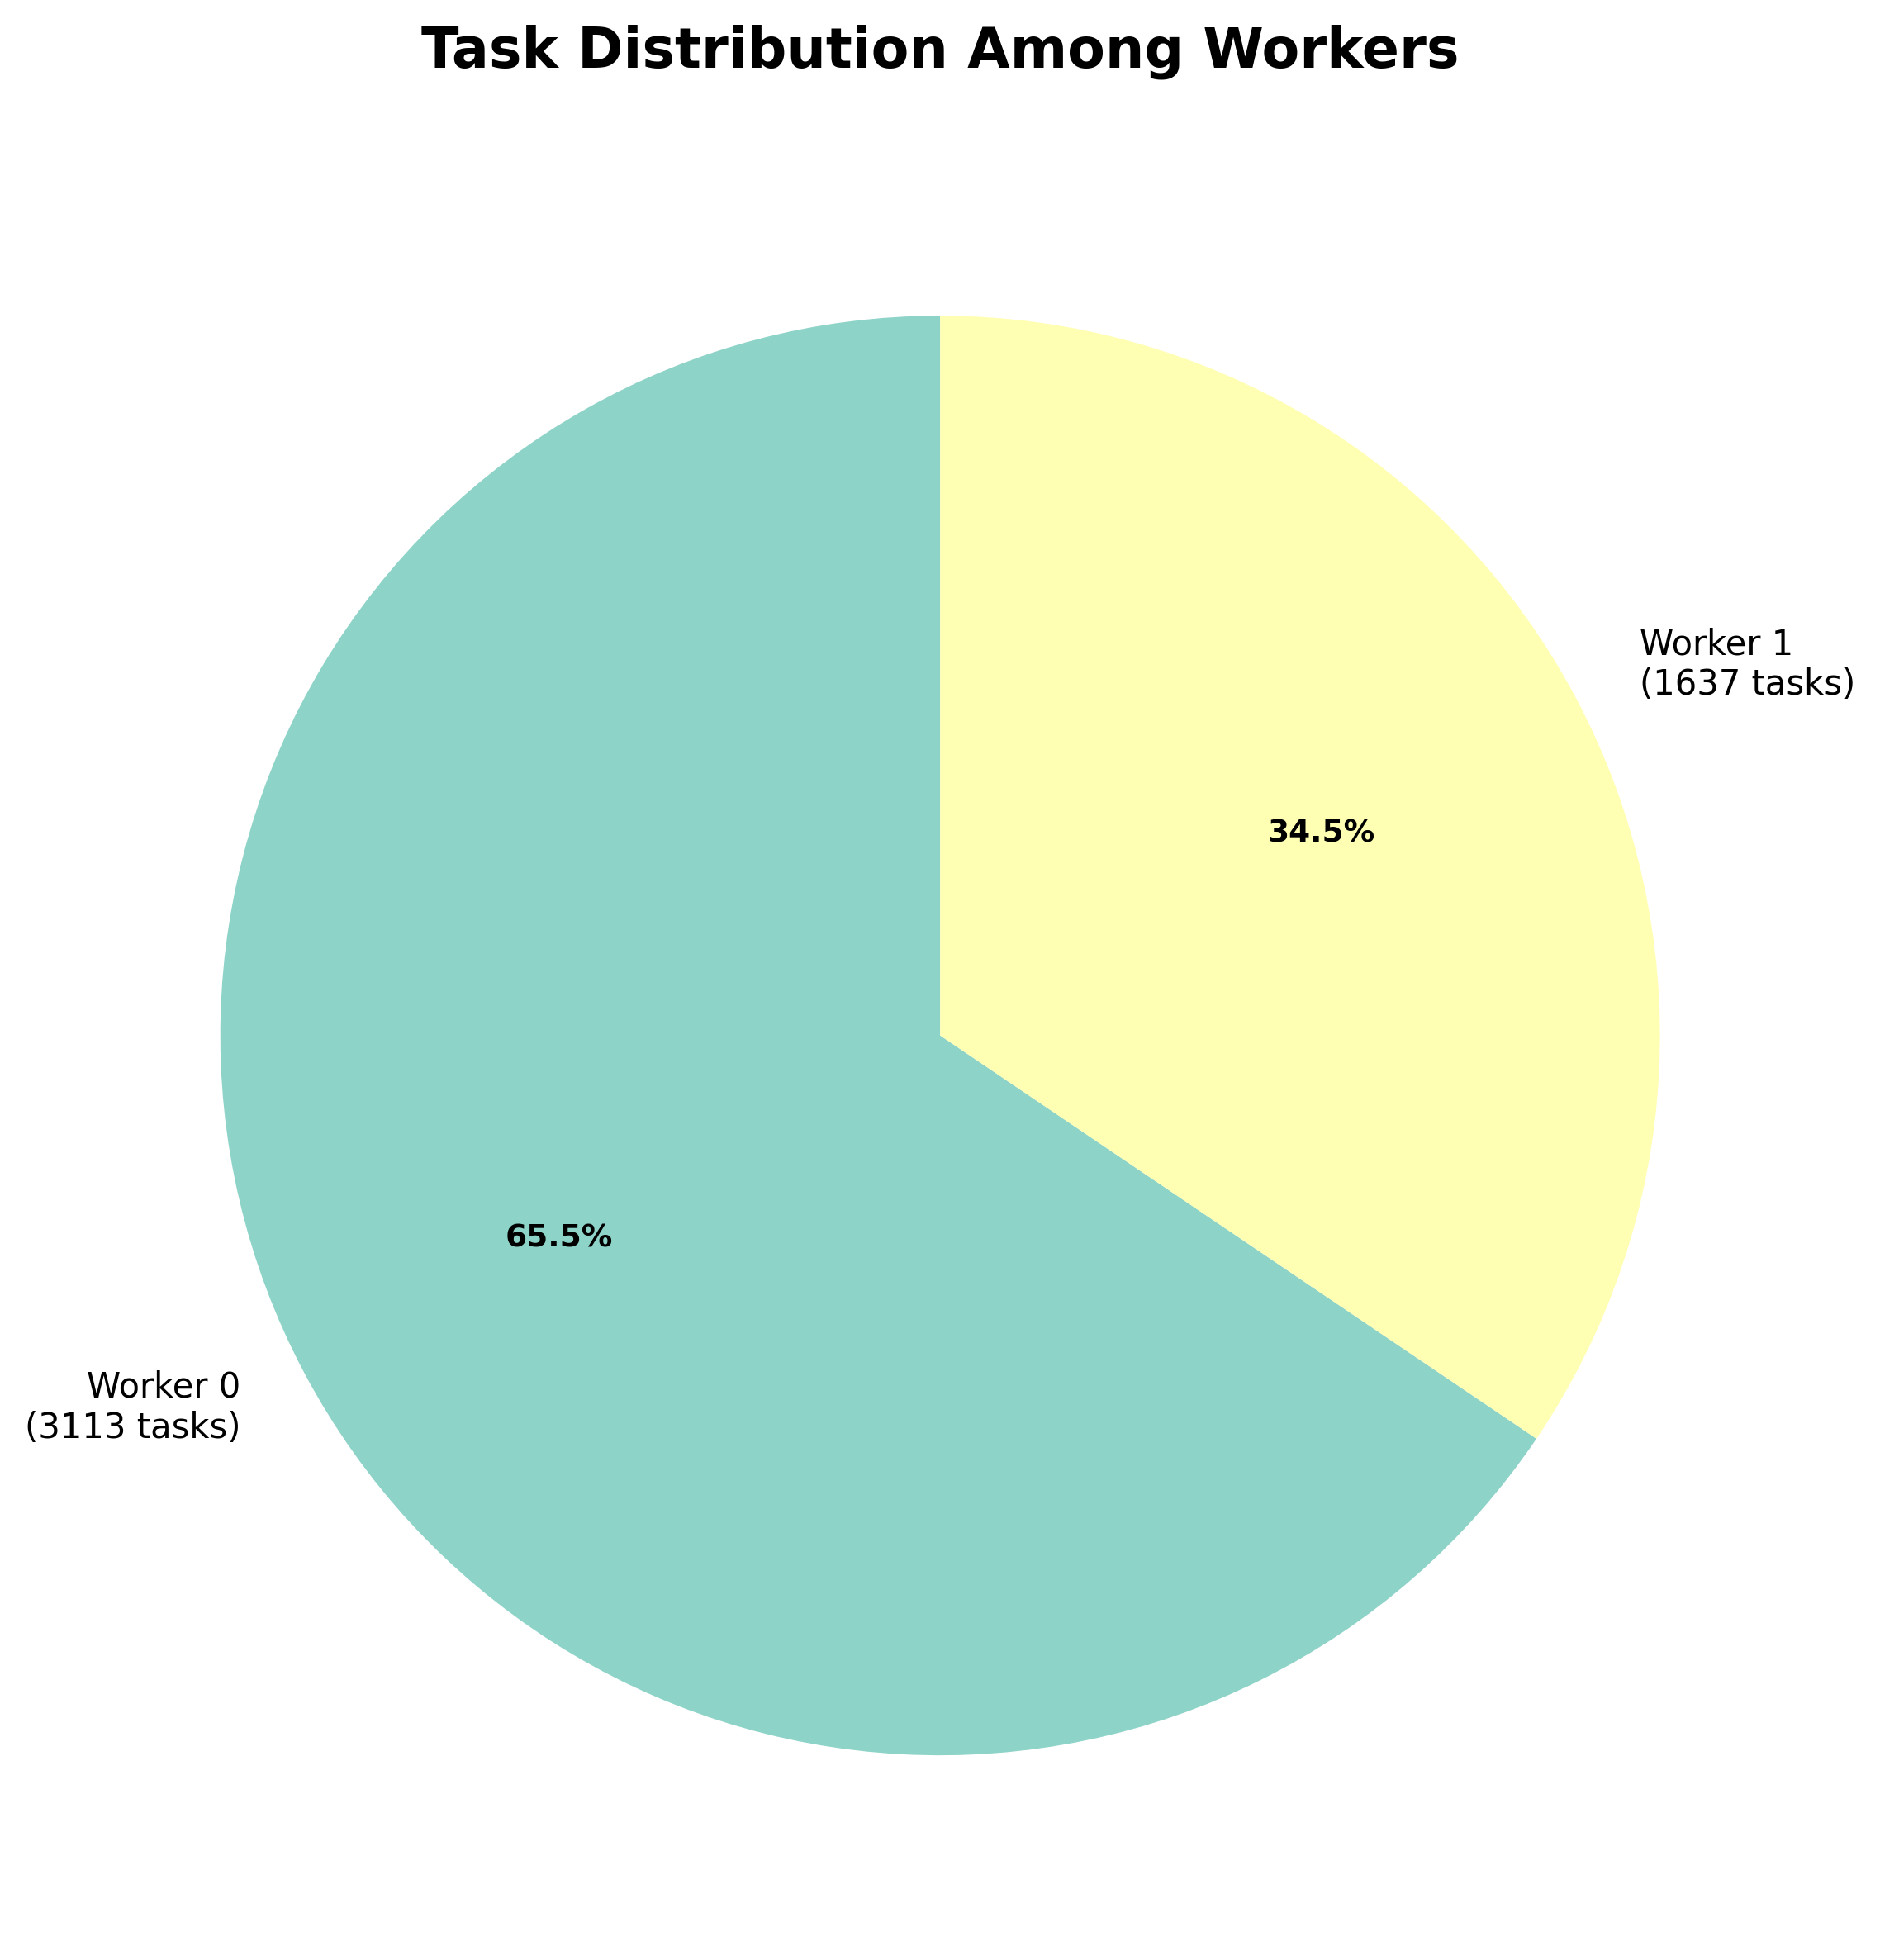
\includegraphics[width=0.5\textwidth]{img/results/variable_computational_budget_sim/active_inference_relative_control_task_distribution_pie.png}
    \caption{AIF – Task Distribution (Budget)}
\end{figure}
\begin{figure}[h]
    \centering
    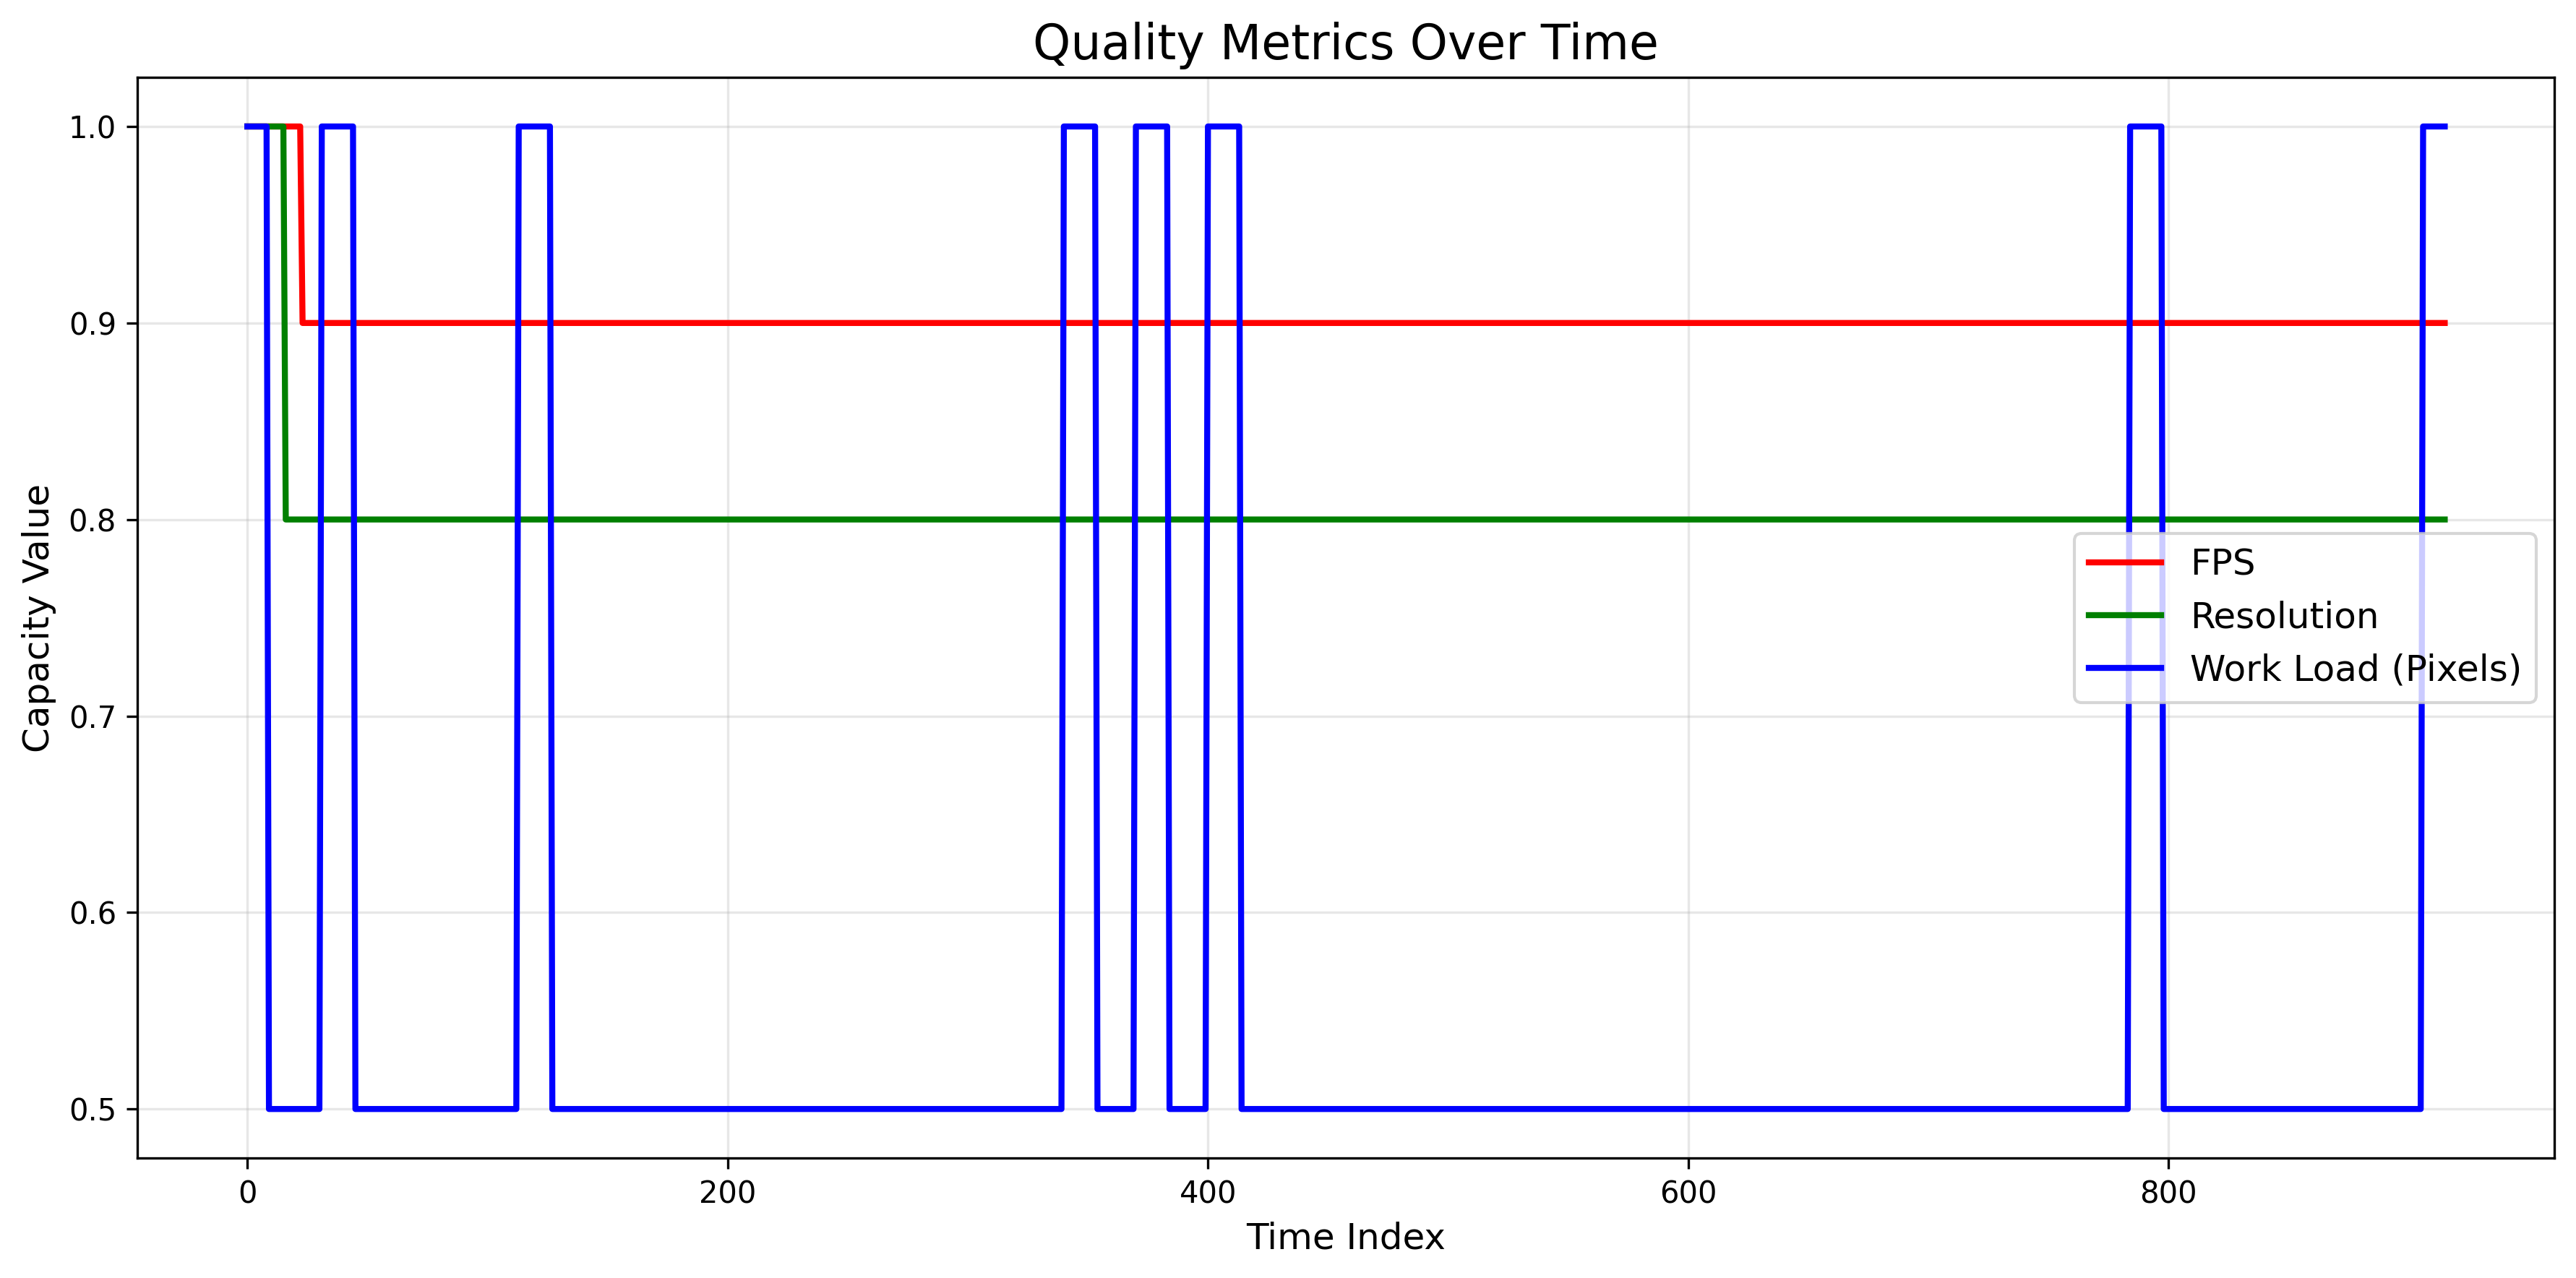
\includegraphics[width=\textwidth]{img/results/variable_computational_budget_sim/heuristic_quality_metrics.png}
    \caption{Heuristic – Quality Metrics Over Time (Budget)}
\end{figure}
\begin{figure}[h]
    \centering
    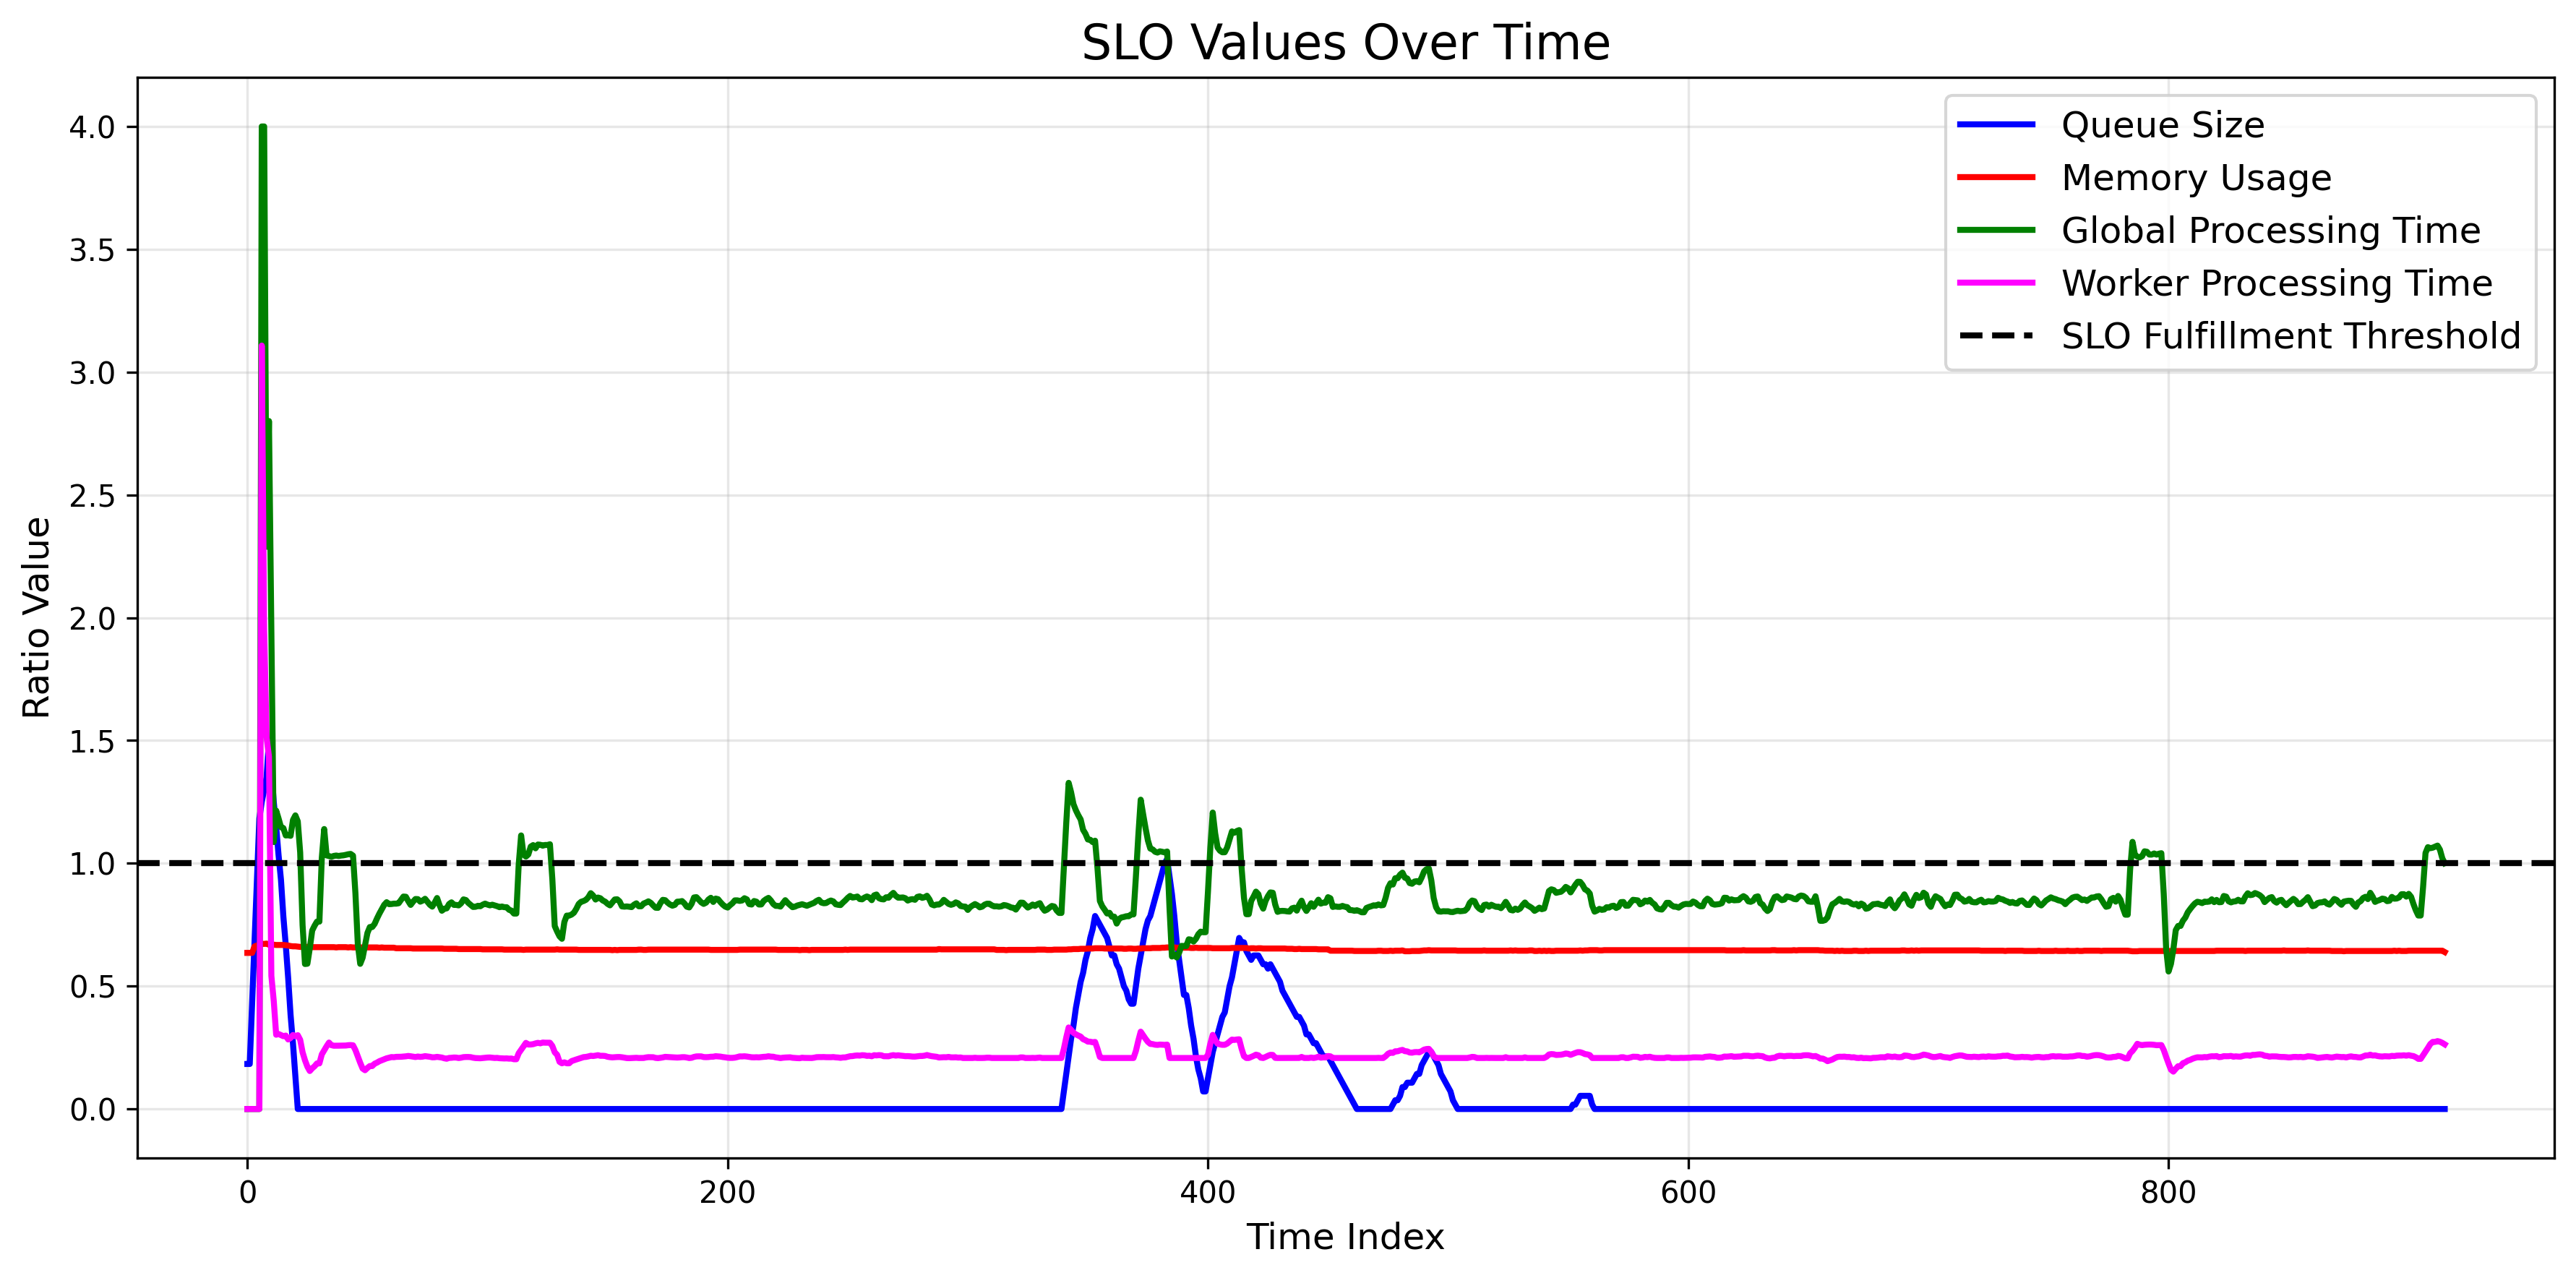
\includegraphics[width=\textwidth]{img/results/variable_computational_budget_sim/heuristic_slo_values.png}
    \caption{Heuristic – SLO Metrics Over Time (Budget)}
\end{figure}
\begin{figure}[h]
    \centering
    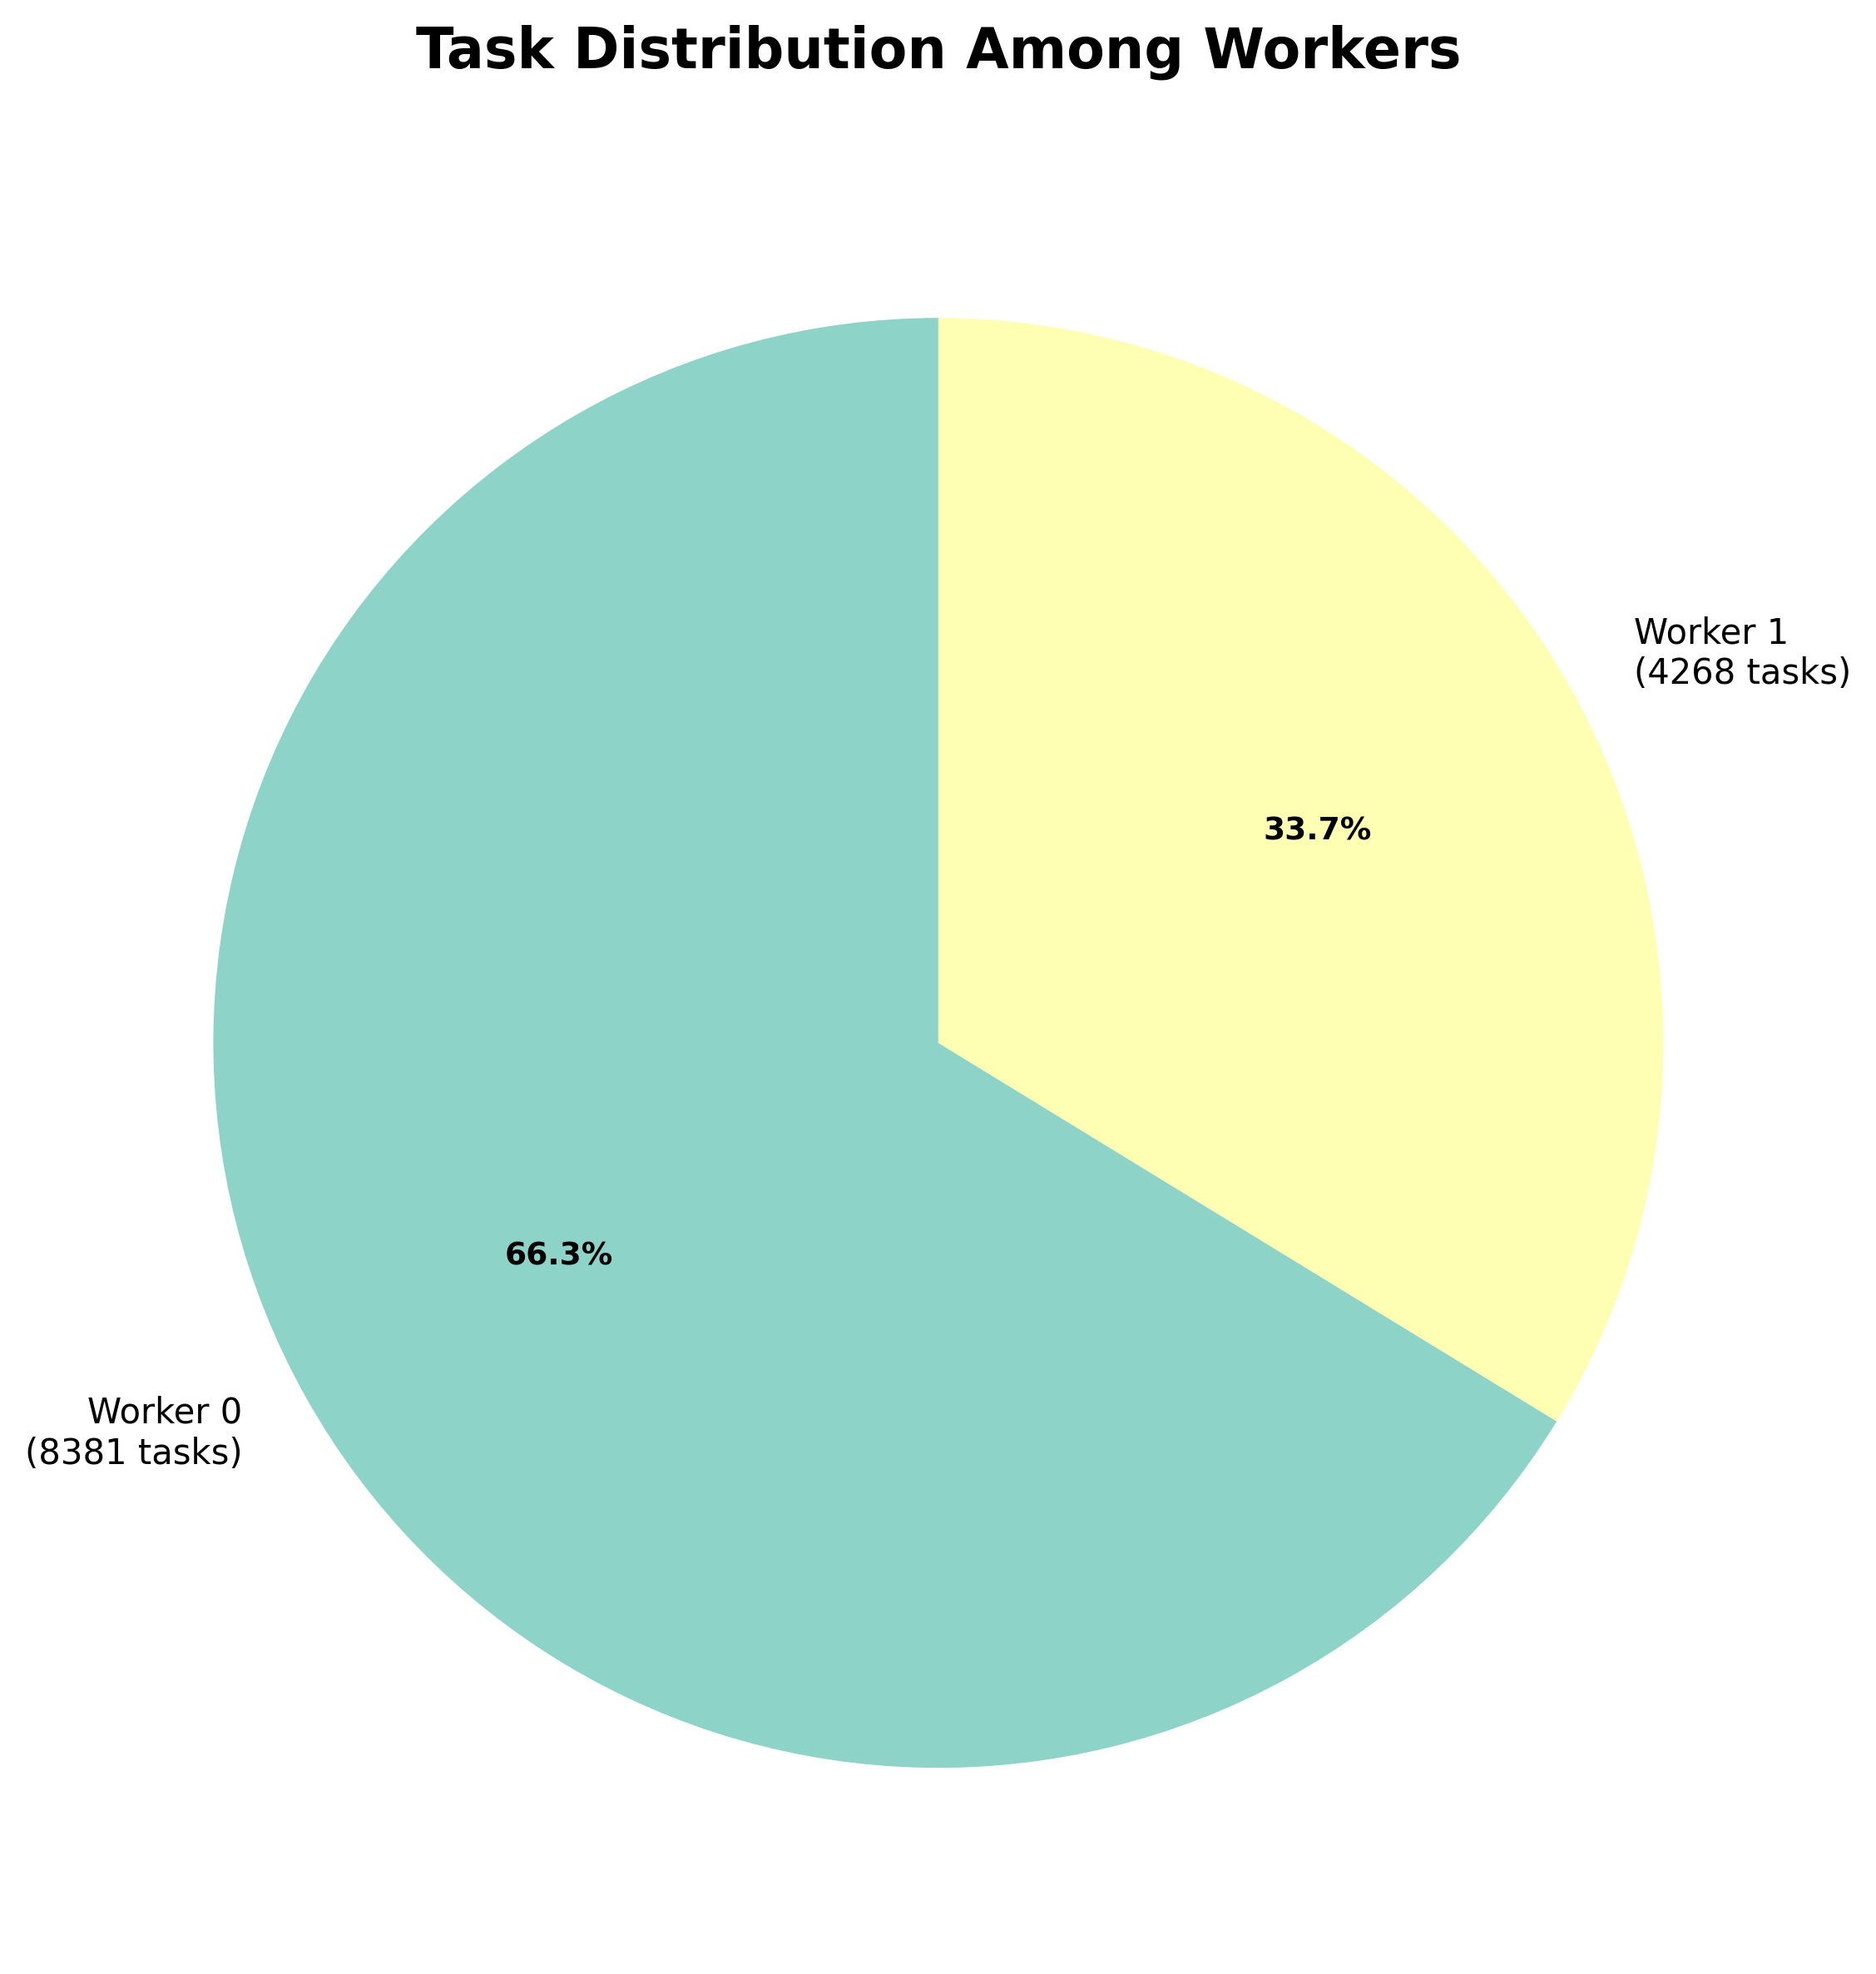
\includegraphics[width=0.5\textwidth]{img/results/variable_computational_budget_sim/heuristic_task_distribution_pie.png}
    \caption{Heuristic – Task Distribution (Budget)}
\end{figure}


\end{document}